\documentclass[twoside]{article}

\usepackage{aistats2026}
% \usepackage[accepted]{aistats2026}   % camera-ready
% \usepackage[preprint]{aistats2026}   % non-anonymous preprint

\usepackage[round]{natbib}
\renewcommand{\bibname}{References}
\renewcommand{\bibsection}{\subsubsection*{\bibname}}

\usepackage{amsmath,amssymb,amsthm,bm,mathtools}
\usepackage{graphicx}
\usepackage{booktabs,multirow,array,longtable}
\usepackage{subcaption}
\usepackage{xcolor}
\usepackage{microtype}
\usepackage{enumitem}
\PassOptionsToPackage{hyphens}{url}
\usepackage[colorlinks=true,linkcolor=blue!60!black,citecolor=blue!60!black,urlcolor=blue!60!black]{hyperref}
\usepackage[capitalise,noabbrev]{cleveref}

\graphicspath{{figures/}}
% let tall two-column tables sit at the top of a text page instead of queuing to the end
\renewcommand{\dbltopfraction}{0.95}
% ---------------------------------------------------------------------------
% Notation and editorial macros for the DISCELL manuscript
% ---------------------------------------------------------------------------
\newcommand{\needsource}{\textcolor{red}{\textbf{[NEEDS A SOURCE]}}}
\newcommand{\todo}[1]{\textcolor{orange}{\textbf{[TODO: #1]}}}
\newcommand{\pending}[1]{\textcolor{violet}{\textbf{[PENDING RUNS: #1]}}}
% editorial flags (kind: note), teal on light cyan; soul's \hl lets a long note break across lines
\newif\ifshowflags \showflagstrue % set \showflagsfalse to hide every editorial flag
\usepackage{soul}
\colorlet{flagbg}{cyan!12}
\DeclareRobustCommand{\flag}[2]{\ifshowflags\leavevmode{\sffamily\bfseries\footnotesize\color{teal!80!black}\sethlcolor{flagbg}\hl{[#1: #2]}}\space\fi\ignorespaces}
% reading-order markers: bold white on teal, [R N]; shown only with \showflagstrue
\DeclareRobustCommand{\readorder}[1]{\ifshowflags\leavevmode{\sffamily\bfseries\footnotesize\setlength{\fboxsep}{1.5pt}\colorbox{teal!80!black}{\textcolor{white}{[R~#1]}}}\space\fi\ignorespaces}

% vocabulary of the generated tables (shared by both manuscripts): AISTATS words; ../recomb/macros.tex defines the RECOMB ones
\newcommand{\termSpill}{leakage}
\newcommand{\TermSpill}{Leakage}
\newcommand{\termSpillFrac}{leak fraction}
\newcommand{\TermSpillFrac}{Leak fraction}
\newcommand{\termReloc}{transport}
\newcommand{\TermReloc}{Transport}
\newcommand{\termInflux}{foreign influx}
\newcommand{\TermInflux}{Foreign influx}

% operators
\DeclareMathOperator{\sgop}{sg}
\newcommand{\sg}[1]{\sgop\!\left[#1\right]}
\DeclareMathOperator{\KL}{KL}
\DeclareMathOperator{\softmax}{softmax}
\DeclareMathOperator{\Mult}{Multinomial}
\DeclareMathOperator{\Pois}{Poisson}
\DeclareMathOperator{\CE}{CE}
\DeclareMathOperator{\diag}{diag}
\DeclareMathOperator{\logdet}{logdet}
\DeclareMathOperator{\embed}{embed}
\DeclareMathOperator{\onehot}{onehot}
\DeclareMathOperator{\GAT}{GATv2}
\DeclareMathOperator{\I}{I}
\DeclareMathOperator{\E}{\mathbb{E}}
\DeclareMathOperator{\Var}{Var}
\DeclareMathOperator{\corr}{corr}
\DeclareMathOperator{\NMI}{NMI}
\DeclareMathOperator{\simop}{sim}
\newcommand{\att}{\pi}   % attention weight, distinct from the loss weights alpha

% sets and fields
\newcommand{\R}{\mathbb{R}}
\newcommand{\Nat}{\mathbb{N}}
\newcommand{\N}{\mathcal{N}}
\newcommand{\simplex}[1]{\Delta^{#1}}
\newcommand{\nbr}[1]{\mathcal{N}_{#1}}

% vectors
\newcommand{\vx}{\mathbf{x}}
\newcommand{\vy}{\mathbf{y}}
\newcommand{\vz}{\mathbf{z}}
\newcommand{\vw}{\mathbf{w}}
\newcommand{\vc}{\mathbf{c}}
\newcommand{\vv}{\mathbf{v}}
\newcommand{\vu}{\mathbf{u}}
\newcommand{\vB}{\mathbf{B}}
\newcommand{\vI}{\mathbf{I}}
\newcommand{\vPhi}{\boldsymbol{\Phi}}
\newcommand{\vrho}{\boldsymbol{\rho}}
\newcommand{\rhobar}{\bar{\boldsymbol{\rho}}}
\newcommand{\vp}{\mathbf{p}}
\newcommand{\vmu}{\boldsymbol{\mu}}
\newcommand{\vsigma}{\boldsymbol{\sigma}}
\newcommand{\wbreve}{\breve{\mathbf{w}}}
\newcommand{\ybar}{\bar{\mathbf{y}}}
\newcommand{\Phibar}{\bar{\boldsymbol{\Phi}}}
\newcommand{\Sig}{\boldsymbol{\Sigma}}
\newcommand{\Sighat}{\hat{\boldsymbol{\Sigma}}}
\newcommand{\lbar}{\bar{\ell}}
\newcommand{\ephi}{e^{\Phi}}
\newcommand{\Ephi}{E_{\Phi}}
\newcommand{\dz}{d_z}
\newcommand{\dw}{d_w}
\newcommand{\dPhi}{d_{\Phi}}
\newcommand{\alphaz}{\alpha_z}
\newcommand{\alphaw}{\alpha_w}
\newcommand{\alphaa}{\alpha_a}
\newcommand{\mpsi}{m_{\psi}}
\newcommand{\Pen}{\mathrm{Pen}}
\newcommand{\Adv}{\mathrm{Adv}}
\newcommand{\dCE}{\Delta\!\CE}
\newcommand{\um}{\,\mu\text{m}}

\newtheorem{proposition}{Proposition}
\newtheorem{remark}{Remark}
\theoremstyle{definition}
\newtheorem{definition}{Definition}


\begin{document}

\runningtitle{DISCELL}
% \runningauthor{...}

\twocolumn[
\aistatstitle{DISCELL}
\aistatsauthor{Anonymous Author}
\aistatsaddress{Anonymous Institution} ]

\begin{abstract}
  \readorder{1} In targeted in situ spatial transcriptomics, a cell's measured transcriptome mixes its intrinsic state, its response to its microenvironment, and transcripts that were assigned to it but belong to its neighbours. The last two are confounded at first order, since both make a cell's expression predictable from its neighbours' types, and the data bound the leak fraction from above but never from below. We therefore do not estimate it: DISCELL, a variational model that splits a cell's counts into these three parts, the leakage as a mixture over graph neighbours, is refitted on a grid of leak fractions, and every claimed spatial contrast is reported with its breakdown point, the smallest leak fraction that explains it away. A type-conditional adversary strips niche-predictable information from the intrinsic state, and a held-out probe, scored against a permutation floor, measures what remains, in DISCELL and in competing models on the same cells. On four sections of ovarian cancer, lung cancer and paediatric lung, the intrinsic state keeps the cell type and the cell cycle, which the response does not carry, and a nonlinear probe recovers $3.5$ to $5.5\%$ of the within-type variance of neighbour composition from it, less than resolVI and Cellina leave on three sections; MintFlow, fitted on three, leaves less still, but its intrinsic latent is close to a type label (cycle $R^2$ at most $0.06$). All claimed contrasts hold up to the largest leak fraction swept, $0.4$, except the response's lean toward signalling genes on one section (breakdown point $0.2$) and the transported prediction's margin over its leakage part on two ($0.3$ and $0.4$); its margin over its programme part, zero by construction without leakage, is positive in every seed from $0.05$ to $0.2$. At the operating point the response has no usable per-cell channel, so its readouts are largely readouts of a regression on the microenvironment.

\end{abstract}

\section{INTRODUCTION}
\label{sec:intro}

Imaging-based spatial transcriptomics assays such as Xenium \citep{janesick2023} measure thousands of transcripts per cell in situ, at single-cell resolution, over sections containing hundreds of thousands of cells. The appeal is obvious: a cell's expression can be read together with the identity and state of the cells around it, which is the raw material for asking how a microenvironment shapes the cells within it. The difficulty is that a cell's measured count vector is not a clean readout of that cell. It is at least three things superimposed. First, the cell's \emph{intrinsic} state: its type, its cell-cycle phase, its clone-associated expression, and the systemic signals that reach every cell of its type regardless of position. Second, its \emph{response} to the local microenvironment: the programmes that differ with who its neighbours are and what the surrounding tissue architecture looks like. Third, a \emph{measurement artefact} specific to in situ assays: transcripts that were detected in the vicinity of a segmentation boundary and assigned to the wrong cell. Segmentation of densely packed tissue is imperfect, and published estimates place the fraction of misassigned transcripts anywhere between one tenth and one half \needsource.

The second and third components are confounded at first order. A cell whose counts are contaminated by its neighbours acquires their markers; a cell that responds to its neighbours shifts its own programmes in a way their types predict. Where the responding genes are also markers of the neighbouring types, as for many ligands and receptors, or where a programme is shared across a region, the two produce the same signature, and neighbour composition predicts both. That misassigned transcripts produce apparent neighbourhood effects, including spurious cell--cell interaction signals, has been shown directly on in situ data \citep{mitchel2026celladmix}, and the contamination a cell receives grows with the local density of the donor type \citep{bilous2026split}. The two differ in form, one adds a neighbour's own profile, the other shifts the cell's own programmes, but from the cell-by-gene count matrix alone the split between them is fixed only by the parametric forms one is willing to assume, and a flexible decoder can mimic either. Any claim that a spatial effect on expression is real therefore depends, silently, on how much of the neighbour-predictable signal was attributed to contamination.

This paper makes that dependence explicit rather than hiding it. We propose DISCELL (\emph{disentangled cell states}), a generative model of per-cell counts with two latent variables and one fixed mixing operator. A latent $\vz_i$ carries the cell's intrinsic state and is, by architecture and by regularisation, pushed to carry no information about the microenvironment given the cell's type; a held-out probe measures how much remains. A latent $\vw_i$ carries the variation associated with a deterministic context descriptor $\vc_i$ that summarises who and what is nearby. A sparse, precomputed leakage kernel $\beta$ mixes a fraction $\kappa$ of each neighbour's clean expression profile into the cell's expected composition. In the decomposition usual for spatial expression, into intrinsic, spatial, niche, technical and noise terms, the model reads
\begin{equation*}
\begin{aligned}
\vx_i \mid \ell_i &\sim \Mult(\ell_i, \vp_i),\\
\vp_i &= (1-\kappa)\,\softmax\big(\underbrace{a(\vz_i)}_{\text{intrinsic}} + \underbrace{\vB\vw_i}_{\text{niche}}\big) + \underbrace{\kappa\,\rhobar_i}_{\text{leakage}},
\end{aligned}
\end{equation*}
where $\rhobar_i = \sum_j \beta_{ij}\vrho_j$ is the neighbours' clean composition. Two technical terms are handled here: the leakage, and the depth $\ell_i$, which is conditioned on; the multinomial is the counting noise. The spatial field has no term of its own: variation at the scale of a tissue domain reaches $\vw_i$ through the image descriptor in $\vc_i$ and is attributed to the niche. Ambient RNA and batch are not modelled, and each fit is one section. The leak fraction $\kappa$ is not estimated. It is fixed, the model is refitted on a grid of $\kappa$ values, and every spatial effect is reported as a function of $\kappa$ with its envelope over random seeds, a sensitivity analysis in which $\kappa$ is the sensitivity parameter. For each effect we report the smallest leak fraction at which it breaks down: an effect that survives the whole grid cannot be explained by leakage of the modelled form, and one that breaks down at the first leak fraction above zero is not separable even from that. The range across the grid is the deliverable, reported alongside an operating point. It is not a confidence interval, and it does not shrink with more cells.

Our modelling choices follow from three requirements that we motivate in \cref{sec:method} and \cref{app:rationale}. The decoder receives no type label, so that $\vz$ is forced to carry identity and cannot degenerate into a residual code. The context encoder queries the neighbourhood with the cell's type rather than with $\vz_i$ and reads only the neighbours' types, closing a channel through which attention would otherwise reconstruct the cell from its most similar neighbours and make the prior on $\vw$ ego-informed. And the invariance we enforce is \emph{conditional} on type: cell types cluster in space, so a marginal invariance between $\vz$ and neighbourhood composition deletes cell type from $\vz$ altogether, the trade-off known from demographic parity \citep{zhao2019inherent} and observed for conditional subspace VAEs \citep{slavutsky2025}.

\paragraph{Related work.}
Classical models separate these components by the dependence structure each is assumed to have. Variance-component models decompose each gene's variance: SpatialDE \citep{svensson2018spatialde} into a spatially smooth and a non-spatial part with a Gaussian process over coordinates, and SVCA \citep{arnol2019svca} further into intrinsic, environmental and cell--cell interaction components, the last driven by the neighbours' expression. Nonnegative spatial factorisation \citep{townes2023nsf} and MEFISTO \citep{velten2022mefisto} place Gaussian-process priors on latent factors instead. Regression and attribution models tie expression to niche covariates: C-SIDE \citep{cable2022cside} estimates cell-type-specific effects of spatial covariates while modelling the mixture of types within a spot, and MISTy \citep{tanevski2022misty} scores how much of a marker is explained by the cell's own markers, its immediate neighbours and the wider tissue. Contamination is handled separately, by correcting the counts before any analysis. SoupX, DecontX and CellBender remove ambient RNA \citep{young2020soupx,yang2020decontx,fleming2023cellbender}. SpotClean removes spot swapping on array-based assays with one bleeding rate per slide and a Gaussian distance kernel, both estimated with the help of spots outside the tissue \citep{ni2022spotclean}, which is the closest precedent for our single leak fraction; in situ assays have no such spots, which is one reason we sweep the fraction instead. Baysor segments cells from the transcript positions themselves \citep{petukhov2022baysor}, and admixture correction removes misassigned transcripts after segmentation \citep{mitchel2026celladmix}. The separation these models achieve rests on assumed dependence structures, which makes it transparent; what they do not provide is a generative model of the cell in which a response to the niche and leakage from it compete for the same counts, and they treat contamination as a preprocessing step rather than as part of the model whose effects are being read.

Node-centric expression models \citep{fischer2023} regress a cell's expression on its neighbourhood directly and produce a niche descriptor without a per-cell latent; our context descriptor $\vc_i$ plays that role, and $\vw_i$ is what remains after conditioning on it. Several models share our design goal of separating intrinsic from spatially associated variation. SIMVI \citep{dong2025simvi} splits a cell's state into an intrinsic and a spatially induced part with an independence regulariser; MintFlow \citep{akbarnejad2025mintflow} conditions an intrinsic latent on cell type and a microenvironment latent on neighbour-type composition, and discourages the former from predicting the latter with type-specific discriminators; Celcomen \citep{megas2026celcomen} separates intra- from inter-cellular gene-interaction programmes with a generative graph neural network; NicheCompass \citep{birk2025nichecompass} characterises niches with a graph neural network; and Cellina \citep{moeed2026cellina} encodes an intrinsic latent from the cell's counts and an extrinsic one from its neighbours' expression, ties the former to cell type with a classifier, removes spatial-domain labels from it adversarially, and evaluates the split by predicting expression under a swapped neighbourhood. None of them models transcript leakage, the confound this paper is about, and MintFlow and Cellina name segmentation errors as a limitation \todo{verify the NicheCompass characterisation; add scVIVA and further spatial VAEs}. Contamination-aware models for in situ data, notably resolVI \citep{ergen2025}, write a cell's counts as a mixture of its own decoded expression, its neighbours' expression decoded by the same network and weighted under a distance-kernel prior, and a slide-wide background, and estimate the mixing and neighbour weights per cell. Our leakage term is the same neighbour-mixing construction with the weights fixed, one leak fraction per section and no background term. We also adopt resolVI's stop-gradient on the neighbour path, which it uses for training stability, and describe the degeneracy it prevents (\cref{sec:batching}). resolVI separates the components by expecting true expression to be low-dimensional. A response to the neighbourhood is low-dimensional too, and the part of it that moves a cell toward its neighbours' profile has the same effect as leakage, so that expectation no longer separates the two on its own; we therefore sweep the leak fraction rather than estimate it \todo{support with the planted-leakage synthetic run once the synthetic appendix returns}. Variational disentanglement of condition-specific from shared representations \citep{klys2018,slavutsky2025} supplies the two-bound objective and the posterior-regularisation view of an adversarial invariance term \citep{ganchev2010} that we build on. We depart from them in three ways. The condition is not an observed label but the cell's niche, summarised by a deterministic context descriptor on which the prior of $\vw$ is conditioned. The invariance is conditional on cell type rather than marginal, because type and niche are dependent in tissue, as is standard in fair and domain-invariant representation learning \citep{madras2018,li2018ciddg,pogodin2023circe}. And our intrinsic path keeps the full decoder and draws $\vw$ from its prior instead of decoding from $\vz$ alone (\cref{app:pathb}). Our invariance target is a fixed data descriptor of the niche, so the model cannot shape it to make invariance trivial, unlike an independence penalty between two learned latents \citep{dong2025simvi}. That adversarial removal is not sufficient without an independent check is the observation of \citet{elazar2018}; our probe protocol is its application. \todo{extend related work: further spatial VAEs and GNN spatial models} \Cref{tab:related} compares the closest models on the properties this paper turns on.

\begin{table*}[t]
\centering
\caption{The models closest to DISCELL, compared on the properties this paper turns on. \emph{Intrinsic latent}: a per-cell latent for the cell's own state. \emph{Niche term}: a component of the model that depends on the neighbourhood. \emph{Leakage}: misassigned transcripts are part of the generative model; \emph{leak share}: how the amount of leakage is set. \emph{Invariance}: the regulariser that keeps the intrinsic latent free of the niche, and whether it conditions on type. \emph{Counterfactuals}: expression predicted under an intervention. $\checkmark$: yes; $\times$: no; --: not applicable.}
\label{tab:related}
\small
\setlength{\tabcolsep}{4pt}
\begin{tabular}{@{}>{\raggedright\arraybackslash}p{0.14\textwidth}>{\centering\arraybackslash}p{0.07\textwidth}>{\raggedright\arraybackslash}p{0.15\textwidth}>{\centering\arraybackslash}p{0.07\textwidth}>{\raggedright\arraybackslash}p{0.11\textwidth}>{\raggedright\arraybackslash}p{0.17\textwidth}>{\raggedright\arraybackslash}p{0.15\textwidth}@{}}
\toprule
Model & Intrinsic latent & Niche term & Leakage & Leak share & Invariance & Counterfactuals \\
\midrule
resolVI \citep{ergen2025} & $\checkmark$ & $\times$ & $\checkmark$ & estimated per cell & $\times$ & $\times$ \\
SIMVI \citep{dong2025simvi} & $\checkmark$ & spatially induced latent & $\times$ & -- & independence, marginal & $\times$ \\
MintFlow \citep{akbarnejad2025mintflow} & $\checkmark$ & microenvironment latent & $\times$ & -- & adversarial, given type & in silico perturbation \\
Celcomen \citep{megas2026celcomen} & $\times$ & inter-cellular gene interactions & $\times$ & -- & -- & gene knockouts \\
Cellina \citep{moeed2026cellina} & $\checkmark$ & extrinsic latent & $\times$ & -- & adversarial against domain labels, marginal & swapped neighbourhoods \\
DISCELL & $\checkmark$ & context-conditional response $\vw_i$ & $\checkmark$ & one per section, swept & adversarial, given type & a changed context, with abduction \\
\bottomrule
\end{tabular}
\end{table*}

\paragraph{Contributions.}
(i) A generative model that decomposes in situ counts into intrinsic state, microenvironmental response and neighbour leakage, with a multinomial likelihood in which the leakage mixture is exact under Poisson sources whose leaked-in rate scales with the receiving cell's own rate rather than the donors' (\cref{sec:generative}). (ii) An inference scheme whose architecture closes information channels that a regulariser cannot reach on its own: the intrinsic encoder never sees the context, the attention context is queried by type, and neighbour quantities are frozen, with an exact two-hop batching scheme that makes the frozen path affordable (\cref{sec:inference,sec:batching}). (iii) A conditional-invariance regulariser, adversarial in its operating configuration with a closed-form penalty as the cheaper first attempt, conditional on type as in the type-specific discriminators of \citet{akbarnejad2025mintflow} but targeting an image-derived niche descriptor alongside neighbour composition, together with a held-out probe protocol that grades either independently of the training objective (\cref{sec:invariance}). (iv) The leakage sweep as a sensitivity analysis: spatial effects are reported as trajectories over $\kappa$ with seed envelopes, alongside an operating point (\cref{sec:sweep}). \todo{(v) the empirical evaluation, to be added}

\section{THE DISCELL MODEL}
\label{sec:method}

We present the model in the order in which its parts depend on one another: the observed quantities and the spatial graph (\cref{sec:setting}); the generative model and the assumptions behind it (\cref{sec:generative}); the inference networks (\cref{sec:inference}); the objective (\cref{sec:objective}); the conditional-invariance regulariser and the held-out probe that grades it (\cref{sec:invariance}); the frozen-neighbour batching that makes the model trainable (\cref{sec:batching}); model selection (\cref{sec:selection}); and what is and is not identified, which is what turns a fit into a finding through the leakage sweep (\cref{sec:sweep}). Each design decision is stated with its reason; the longer arguments are in \cref{app:rationale} and the derivations in \cref{app:derivations}. \Cref{fig:overview} summarises the model for one cell.

\begin{figure*}[t]
\centering
\raisebox{-\height}{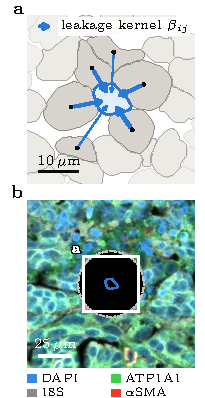
\includegraphics{figures/fig_model_tissue}}\hspace{0.22in}%
\raisebox{-\height}{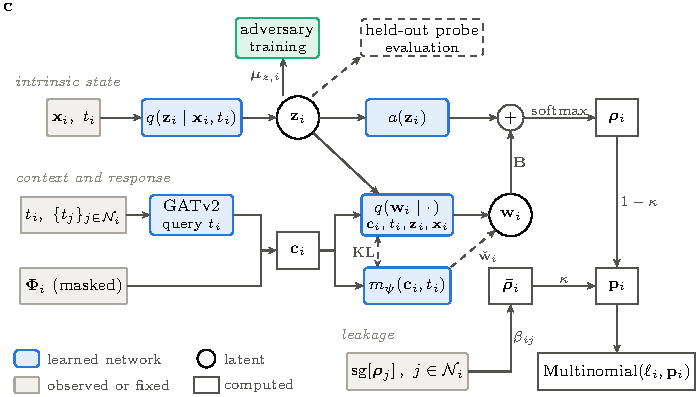
\includegraphics{figures/fig_model_graph}}
\caption{DISCELL for one cell $i$. \textbf{a},~The leakage kernel on the primary section: the cell (blue), its first ring of neighbours in the pruned Delaunay graph (dark grey), each sending an arrow whose width grows with its weight $\beta_{ij}$, and its second ring (light grey), which the batching of \cref{sec:batching} also reads. The attention that builds the context runs over the same first ring but uses no edge features: its weights depend on the two cells' types alone (\cref{eq:context-closed}). \textbf{b},~The input of the image descriptor $\vPhi_i$: the four-channel morphology crop the image model receives ($128\um$ field; the markers DAPI, ATP1A1, 18S and $\alpha$SMA as the image model reads them, shown as one colour composite; on the slide the ATP1A1 channel is a membrane mix with CD45 and E-cadherin, and the $\alpha$SMA channel a mix with vimentin), with the $25\um$ disc over the cell set to zero; the cell's outline is drawn for reference. The square marked~a is the window of panel~a: the zeroed disc covers the cell and most of its first ring, so the descriptor describes the tissue around the leakage neighbourhood rather than the neighbourhood itself. Tissue panels are in image orientation. \textbf{c},~The computation graph. The intrinsic state $\vz_i$ is encoded from the cell's own counts and type. The context $\vc_i$ combines attention over the neighbours' types, queried with the cell's type, with $\vPhi_i$. The response $\vw_i$ has the prior $p(\vw_i \mid \vc_i, t_i)$ with mean $\mpsi$, and a posterior that also sees the cell. The clean composition $\vrho_i = \softmax(a(\vz_i) + \vB\vw_i)$ is mixed with the neighbours' clean compositions, held under a stop-gradient, through $\beta$ and the fixed leak fraction $\kappa$. The dashed $\wbreve_i$ is the prior draw used by the intrinsic path. The adversary acts on the posterior mean $\vmu_{z,i}$ during training; the held-out probe grades it afterwards and never enters training.}
\label{fig:overview}
\end{figure*}

\subsection{Setting and Notation}
\label{sec:setting}

We consider a single tissue section profiled with a targeted in situ assay. For each of $N$ segmented cells $i$ we observe a count vector $\vx_i \in \Nat^G$ over $G$ genes, its total $\ell_i = \sum_g x_{ig}$, a cell-type label $t_i \in \{1,\dots,K\}$, and the morphology image around the cell. The label may be a curated annotation or a frozen unsupervised clustering and is treated as data, with two caveats that recur below: it was itself derived from the same contaminated counts, and its granularity is a modelling choice that sets what the decomposition is relative to (\cref{sec:invariance}). Cells without a label form one additional class. In training it enters every type-conditioned quantity like any other, and its cells remain neighbours of the cells around them. It is never a target of evaluation: every diagnostic and readout of \cref{sec:selection,sec:sweep} is computed on labelled cells only, because a residual class is not a cell type, and a read that treated it as one would measure the failure of the label rather than the model. Curated annotations frequently encode state or location as well as lineage (tumour- versus stroma-associated fibroblasts, hypoxic or proliferating tumour subsets). Such labels are niche-informed: conditioning on them assigns the corresponding response to $t$, where neither $\vw$ nor the invariance of \cref{sec:invariance} sees it. Labels should therefore be lineage-level, with state-bearing subtypes merged before fitting, as they are in every fit reported here. The total $\ell_i$ is conditioned on throughout and never modelled.

\paragraph{Spatial graph.}
Cells are nodes; two cells are adjacent if and only if their Voronoi cells share a face, i.e.\ no third cell lies between them (Delaunay adjacency). This choice has no neighbourhood count $k$ and no radius, adapts to local packing with an average degree near six, and uses only cell centroids, so it is insensitive to segmentation-boundary noise and to the nuclear-expansion segmentation that in situ platforms fall back on. Delaunay adjacency also connects cells across lumens, vessels and tears, so edges longer than a cut-off ($40\um$ here) are pruned. We write $\nbr{i}$ for the pruned neighbour set of $i$, which excludes $i$ itself; all its members are first-order neighbours, so no cell-size correction of distances is needed. The same graph serves every role below.

For each edge we record the centroid distance $d_{ij}$ and the length $f_{ij}$ of the shared Voronoi face, measured after clipping each Voronoi cell to a $30\um$ disc around its centroid so that faces at tissue borders and across gaps are bounded. The face length is a proxy for contact extent that is defined whether or not the segmented polygons touch. We deliberately do not use the length of shared segmented boundary: segmented polygons of adjacent cells rarely touch, so a contact length would vanish on a large share of edges, and where it is non-zero it tracks the gap between polygons, which is local density, a property of the niche that we want to keep out of the \emph{technical} part of the model, the part that describes measurement rather than biology (\cref{app:graph}; \cref{fig:voronoi-face,tab:contact}).

\paragraph{Derived observables.}
From the graph and labels we form the neighbour-type composition $\vy_i \in \simplex{K-1}$, $y_{ik} = |\{j \in \nbr{i} : t_j = k\}| / |\nbr{i}|$, which excludes the cell itself. From the image we form an embedding $\vPhi_i \in \R^{\dPhi}$ of a patch centred on the cell, produced by a frozen pretrained vision model, in which a disc covering the cell has been masked out, so that $\vPhi_i$ describes the surrounding tissue and not the cell (\cref{app:image}). The two descriptors act at different scales: the graph is one hop, a few to thirty micrometres, while the masked patch describes tissue beyond roughly $25\um$; both are what we mean by ``the niche''. Here $\dPhi$ is the embedding's native width; whether a low-dimensional projection should replace it is an open implementation choice (\cref{app:deviations}). Three lookup tables are fixed before training: $\ybar(t)$, the mean composition of cells of type $t$; $\Phibar(t)$, the mean image-niche membership of type $t$; and $\bar{\vv}(t)$, the mean of the invariance block of \cref{sec:invariance} for type $t$. Isolated cells, those with no neighbours after pruning, have an empty composition and are excluded from all three tables.

\paragraph{Leakage kernel.}
The leakage kernel is a sparse matrix over the same edges, normalised over the neighbours of each connected cell,
\begin{equation}
  \beta_{ij} \;\propto\; f_{ij}\,\exp(-d_{ij}/\tau), \qquad \sum_{j \in \nbr{i}} \beta_{ij} = 1,
  \label{eq:beta}
\end{equation}
with contamination decay length $\tau = 20\um$; it is row-stochastic on connected cells, and an isolated cell keeps an all-zero row. It is precomputed once and never learned, which is where it departs from the neighbour-mixing term of \citet{ergen2025}, whose weights are fitted per cell. Continuous geometry is allowed here, and only here: $\beta$ is not part of any conditioning variable and does not touch the estimand (\cref{app:graph}).

\subsection{Generative Model}
\label{sec:generative}

Each cell has two latent variables. The intrinsic state $\vz_i \in \R^{\dz}$ carries what the cell is; the response $\vw_i \in \R^{\dw}$ carries how cells of that type shift with their surroundings. The environment itself enters as a deterministic context descriptor $\vc_i$ (defined in \cref{sec:inference}) that is shared by co-located cells. With $\mpsi$ a learned prior-mean network, $a$ a learned decoder, $\vB \in \R^{G \times \dw}$ a learned loading matrix and $\kappa \in [0,1)$ the fixed leak fraction,
\begin{align}
  \vz_i &\sim \N(\mathbf{0}, \vI), \label{eq:gen-z}\\
  \vw_i \mid \vc_i, t_i &\sim \N\big(\mpsi(\vc_i, t_i),\, \sigma_w^2 \vI\big), \label{eq:gen-w}\\
  \vrho_i &= \softmax\big(a(\vz_i) + \vB\vw_i\big), \label{eq:gen-rho}\\
  \rhobar_i &= \textstyle\sum_{j \in \nbr{i}} \beta_{ij}\, \vrho_j, \label{eq:gen-rhobar}\\
  \vp_i &= (1-\kappa)\, \vrho_i + \kappa\, \rhobar_i, \label{eq:gen-p}\\
  \vx_i \mid \ell_i &\sim \Mult(\ell_i, \vp_i). \label{eq:gen-x}
\end{align}
Here $\vrho_i \in \simplex{G-1}$ is the cell's own \emph{clean} composition, $\rhobar_i$ is the \emph{foreign influx}, the leakage-weighted average of its neighbours' clean compositions, and $\vp_i$ is the fitted multinomial probability. The decoder $a(\vz_i) \in \R^G$ is the cell's baseline programme in log space; column $k$ of $\vB$ is a gene programme and $w_{ik}$ is how far cell $i$ has moved along it. The prior variance is fixed at $\sigma_w = 1$, deliberately (\cref{sec:inference}).

For an isolated cell $\rhobar_i = \mathbf{0}$, and the mixture in \cref{eq:gen-p} would sum to $1-\kappa$, charging the cell $-\ell_i\log(1-\kappa)$ nats for leakage it cannot receive. The mixture is therefore renormalised per row,
\begin{equation}
  \vp_i = \frac{(1-\kappa)\,\vrho_i + \kappa\,\rhobar_i}{(1-\kappa) + \kappa\sum_{j \in \nbr{i}}\beta_{ij}},
  \label{eq:renorm}
\end{equation}
so that an isolated cell degenerates to $\vp_i = \vrho_i$, i.e.\ $\kappa_i = 0$: no neighbours, no foreign source. For connected cells the denominator is one. Probabilities are floored at $10^{-8}$ inside the logarithm. Isolated cells keep an all-zero composition $\vy_i$ and are not excluded from the regulariser or the probes of \cref{sec:invariance}.

\paragraph{What the leakage term assumes.}
The leak fraction $\kappa$ is section-wide, not per cell, and there is no ambient term. A cell's contamination in reality varies with its own size and depth, the depth and density of its neighbours, and how much boundary they share. The model scales the leaked rate with the receiving cell's own rate (below), so a low-count cell beside high-count donors is under-corrected at every $\kappa$, and a high-count cell beside low-count donors over-corrected. The invariance of \cref{sec:invariance} keeps $\vz$ free of anything niche-predictable, so the niche-predictable part of that error is absorbed by $\vw$ and is not addressed by the sweep. Labels are derived from uncorrected counts and held fixed across the grid. Leakage-driven label errors concentrate where leakage is largest, at heterotypic interfaces and in low-count cells beside high-count neighbours; for such a cell the error enters through $t_i$ and through its neighbours' compositions, where neither $\kappa$ nor the invariance reaches it. Diffuse background is assumed negligible relative to leakage from adjacent cells \needsource. The mixture in \cref{eq:gen-p} is exact under two assumptions: that the sources are independent Poisson variables, whose sum is again Poisson, and that the rate of leaked-in transcripts scales with the receiving cell's own rate rather than with the donors', which is where the per-cell variation just mentioned is hidden. The multinomial then follows from conditioning on the observed total (below). The parametrisation also assumes that leakage is gene-agnostic: $\kappa$ carries no gene index, so a leaked transcript is drawn from the donor's whole-cell composition $\vrho_j$. Transcripts nearest the boundary, such as mRNAs of secreted and membrane proteins, are plausibly over-represented in what crosses it \needsource. Such a gene-specific leak is not spanned by $\kappa$ at any value and lands in $\vw$, so a response programme enriched for cell-surface genes cannot be separated from leakage by the sweep alone.

\paragraph{What the decomposition means.}
The split between $\vz$ and $\vw$ is defined by two requirements. First, within a type, the intrinsic state should carry nothing that is predictable from the niche: $\I(\vz_i;\, [\vy_i, \vPhi_i] \mid t_i) = 0$. In \cref{eq:gen-z} $\vz_i$ is a priori independent of everything, and $\vy_i, \vPhi_i$ are not modelled, so this is not a property of the generative model; it is a constraint imposed on the variational family in \cref{sec:invariance}, in the sense of posterior regularisation \citep{ganchev2010}. Second, the environment reaches the counts only through the response and through leakage: $\vx_i \perp \vc_i \mid \vz_i, \vw_i, \{\vrho_j\}_{j \in \nbr{i}}$, which holds by construction because the decoder of \cref{eq:gen-rho} takes no context. Precisely, what the first requirement removes from $\vz$ is variation predictable from the neighbour composition and the masked image given the type. It removes intrinsic variation that is spatially organised within a type only to the extent that neighbour composition and the masked image predict it. On a carcinoma section that extent can be large: subclones occupy contiguous regions and the masked image shows the nuclei of clonal kin, so part of a cell's clone-associated expression is predictable from its niche, is moved from $\vz$ into $\vw$, and would be read as a response; the part they do not predict stays in $\vz$, as does variation carried by the neighbours' own intrinsic codes. How much is at stake depends on the labels as well: a label that splits subclones keeps them in $t$, while under the lineage-level labels recommended above they are within-type variation, and on a carcinoma section this is then the main case rather than a corner case. This is why the decomposition is relative to $t$ (\cref{sec:invariance}).

\paragraph{Why a multinomial.}
If $x_{ig} \sim \Pois(\lambda_{ig})$ independently, then $\vx_i \mid \sum_g x_{ig} = \ell_i$ is $\Mult(\ell_i, \boldsymbol{\lambda}_i / \sum_g \lambda_{ig})$. Since $\ell_i$ is observed, the multinomial is the coherent likelihood: no library-size latent and no double counting of depth. Poisson sources are closed under addition, which is what makes the leakage mixture exact; negative-binomial sources with gene-specific means are not in general, and a negative binomial on the mixed counts would let the dispersion absorb part of what the mixture should explain. At the depth of in situ data, tens to a few hundred counts over thousands of genes, gene-wise overdispersion cannot be estimated in any case, and a low-dimensional amortised $\vz$ absorbs much of what a dispersion parameter captures in coarser models. Should posterior predictive checks show overdispersion at higher depth, the appropriate extension is a Dirichlet-multinomial with one concentration scalar, not $G$ dispersions.

\paragraph{Why $\kappa$ is fixed.}
Leakage and response differ in form: one adds a neighbour's own profile through a fixed contact kernel, the other shifts the cell's own programmes along learned directions. From the cell-by-gene count matrix alone, however, the split between them is pinned only by those parametric forms, and a decoder flexible enough to fit the data can mimic either, since neighbour composition predicts both. The likelihood alone cannot choose $\kappa$: the data bound it from above but not from below (\cref{prop:kappa-bound}). Instead we fix it, fit the model independently at every point of a grid, and report each readout as a function of $\kappa$ (\cref{sec:sweep}). $\kappa = 0$ is the nested no-correction null. The grid is anchored at zero and extends to $0.4$, close to the upper range of published misassignment estimates for this platform \needsource; a data-driven upper bound from an atlas-defined marker set, and the transcript-level information that would identify $\kappa$ from a nuclear/extranuclear split of the counts, are discussed in \cref{app:kappa}.

\paragraph{Why the decoder has no type input.}
The decoder in \cref{eq:gen-rho} takes $\vz_i$ and $\vw_i$ only, so the only route from identity to expression runs through $\vz$. If $\vz$ collapsed to a function of the label, both reconstruction terms in \cref{sec:objective} would lose all within-type variance, a large fitting penalty, and that is what holds $\vz$ open. With the label in the decoder, $\vz$ would become a residual-only code and would no longer be interpretable as identity. What $\vz$ carries beyond the label is what the label discretises away: cell-cycle phase, clone-associated expression, position on a differentiation continuum, stress and metabolic state, states acquired in a niche the cell has since left, and systemic signals that affect every cell of a type regardless of position. The last is environmental in the colloquial sense but not niche-predictable, and it belongs in $\vz$. Two remarks follow. Since the encoder of \cref{sec:inference} receives the label, the agreement between $\vz$ and $t$ measures whether $\vz$ \emph{retains} type, not whether it discovers it; its collapse is the detector for the marginal-invariance failure mode (\cref{sec:selection}). And coarse labels leave more for $\vz$ to carry; whether $\vz$ separates cell-cycle phases within a type is an empirical check for the evaluation.

\subsection{Inference Networks}
\label{sec:inference}

\Cref{tab:learned} summarises what is learned and what is fixed. All networks are multilayer perceptrons unless stated; widths are in \cref{tab:architecture}.

\begin{table}[t]
\centering
\caption{Learned and fixed quantities. $\dz = 20$, $\dw = 6$; $G$, $K$ and $\dPhi$ are set by the panel, the label set and the image model.}
\label{tab:learned}
\small
\begin{tabular}{@{}p{0.47\columnwidth}p{0.47\columnwidth}@{}}
\toprule
Learned & Fixed before training \\
\midrule
encoder of $q(\vz_i \mid \vx_i, t_i)$; attention layer and type query $\embed(t)$; prior mean $\mpsi$; encoder of $q(\vw_i \mid \cdot)$; decoder $a$; loadings $\vB$; adversary heads (separate optimiser) &
graph, kernel $\beta$, $\tau$; leak fraction $\kappa$ (swept); prior scale $\sigma_w = 1$; image embedding $\vPhi$ and its principal components; image-niche memberships $\ephi$; tables $\ybar(t)$, $\Phibar(t)$, $\bar{\vv}(t)$; labels $t$; totals $\ell$ \\
\bottomrule
\end{tabular}
\end{table}

\paragraph{The context descriptor $\vc_i$.}
One vector per cell summarising who and what is nearby. It is deterministic, is shared by co-located cells, and is the conditioning variable of the model. It is computed by a single graph-attention layer \citep{brody2022} over the pruned graph, concatenated with the image embedding and an isolation flag:
\begin{align}
  \mathbf{h}_j &= \onehot(t_j), \label{eq:context-src}\\
  \mathbf{g}_i &= \GAT\big(\text{query} = \embed(t_i),\; \{\mathbf{h}_j\}_{j \in \nbr{i}}\big), \label{eq:context-gat}\\
  \vc_i &= \mathbf{g}_i \;\oplus\; \vPhi_i \;\oplus\; \mathbf{1}[\nbr{i} = \emptyset]. \label{eq:context}
\end{align}
Here $\embed(t_i)$ is a learned per-type vector of width $K$, the width of the source features; since the layer applies its own linear map to the query, this is equivalent to a one-hot query and is a parameterisation, not a design choice. The layer has no self-loops, no edge features, and its heads are averaged. Its attention weights $\att_{ij}$ satisfy $\sum_j \att_{ij} = 1$. The context is therefore a pure function of data, types, graph and image; no latent enters it. With types as both query and sources, the logit of an edge depends on the two types alone, so the attention output is a learned, type-specific reweighting of the neighbour composition, and $\vc_i$ is a fixed function of $(t_i, \vy_i, \vPhi_i)$: the descriptors against which $\vz$ is made invariant, so the prior on $\vw$ sees exactly what $\vz$ is kept from (\cref{app:graph}). Three decisions here are load-bearing.

\emph{The query is the type, not $\vz_i$.} In attention of this form the destination feature enters the attention logits but never the aggregated value, so using $\vz_i$ as the query would inject no ego content directly. It would, however, open a selection channel: attention can learn $\att_{ij} \propto \exp(\simop(\vz_i, \vz_j))$ and reconstruct the cell through its most similar neighbours, so that $\vc_i$ becomes a mirror of $\vz_i$. The incentive exists because an ego-informed prior on $\vw_i$ is free decoder capacity, and it is strongest in homotypic regions, where $\kappa$ is also least identified. The consequence would be that $\mpsi$ already knows the cell, the divergence $\KL(q(\vw_i)\,\|\,p(\vw_i \mid \vc_i, t_i))$ collapses, and $\vw_i$ measures deviation from \emph{self} rather than from the expected response. Querying with the type closes the selection channel at no cost to the prior, since $\mpsi(\vc_i, t_i)$ already receives $t_i$. The sources are the neighbours' types only. An earlier version also fed the neighbours' posterior means under a stop-gradient; removing them improved held-out reconstruction, type agreement and the mirror diagnostic in a three-seed ablation while leaving the response's spatial readouts unchanged, so the input bought nothing measurable and was dropped. The within-type mirror coefficient is still monitored rather than assumed away (\cref{sec:selection}; \cref{app:mirror}).

\emph{No per-edge geometry enters the context.} The graph says who is adjacent; the image describes how packed and how structured the region is; per-edge distances and contact extents are withheld from $\vc_i$. Three reasons, in decreasing order of weight. The concrete risk is collinearity: an attention layer given edge features can rediscover the leakage kernel $\beta$, after which $\vw$ becomes collinear with $\rhobar$ and the two mechanisms the sweep is meant to separate merge inside the model (\cref{app:graph}). Within a first-order neighbourhood the distances span perhaps $5$ to $30\um$, most of which is local density, which the image already carries. And the intended reading of the context is that neighbour-type composition is the exposure of interest while the image and the graph are conditioning covariates; a hypothetical change in composition is a meaningful question about a tissue in a way that ``the same neighbours, further away'' is not, and putting per-edge geometry into the conditioning variable would mix the two. The estimand is used only informally here; counterfactual machinery is future work (\cref{sec:conclusion}).

\emph{Isolated cells.} A cell with no in-edges has an empty attention set; the graph part of $\vc_i$ is set to zero and the flag is raised. The image part stays, since $\vPhi_i$ is measured data defined for every cell. Together with \cref{eq:renorm}, an isolated cell is modelled with $\kappa_i = 0$ and an image-only context.

\paragraph{Posterior over $\vz$.}
The posterior $q(\vz_i \mid \vx_i, t_i)$ is a diagonal Gaussian produced by a network whose input is the library-normalised, log-transformed count vector together with the log total and the one-hot type,
\begin{equation}
  \big[\log(1 + \vx_i\, \tilde\ell / \ell_i),\; \log \ell_i,\; \onehot(t_i)\big], \qquad \tilde\ell = \operatorname{median}_i \ell_i.
  \label{eq:encz-input}
\end{equation}
The encoder \emph{never sees} $\vc_i$: invariance by architecture, which the regulariser of \cref{sec:invariance} then completes. Library normalisation before the log matters because a raw $\log(1+\vx)$ entangles depth with composition, so that a 300-count and a 50-count cell of the same type look very different; since $\ell_i$ is conditioned on rather than modelled, $\vz$ should not spend capacity on it. Total counts are nonetheless weakly informative about state, so $\log \ell_i$ enters as one extra scalar rather than being discarded.

\paragraph{Prior and posterior over $\vw$.}
The prior is what a typical cell of this type would do in this context; the posterior is what this cell did:
\begin{align}
  p(\vw_i \mid \vc_i, t_i) &= \N\big(\mpsi(\vc_i, t_i),\, \sigma_w^2 \vI\big), \label{eq:prior-w}\\
  q(\vw_i \mid \vc_i, t_i, \vz_i, \vx_i) &= \N\big(\vmu_{w,i},\, \diag \boldsymbol{\nu}_{w,i}^2\big), \label{eq:post-w}
\end{align}
with $\boldsymbol{\nu}_{w,i}$ the learned posterior scale, as distinct from the fixed prior scale $\sigma_w$. Both distributions are functions of the context, but only the posterior sees the cell itself, through the sampled $\vz_i$ and through the encoded counts of \cref{eq:encz-input}; we abbreviate the posterior as $q(\vw_i)$ where its arguments are clear. The divergence $\KL(q \,\|\, p)$ reads as how far this cell deviates from its expected response, an anomaly score that the objective provides at no extra cost; whether it carries usable per-cell information at the operating point is an empirical question for the evaluation. The prior is also what would make counterfactuals possible, by drawing $\vw' \sim p(\vw \mid \vc', t)$ and decoding, with abduction $\vw'_i = \vw_i + \mpsi(\vc', t_i) - \mpsi(\vc_i, t_i)$ carrying the cell's own residual unchanged: because the prior scale is fixed, the per-cell counterfactual is exactly a translation of the prior mean, and the difference $\vw'_i - \vw_i$ is manifestly free of the per-type gauge of \cref{sec:sweep}. The type-level form of this machinery, in which the prior mean alone is moved to a new context and the cell's intrinsic state is held fixed, is exercised in the evaluation; the per-cell form with abduction is not, since it presupposes a non-degenerate response posterior.

The direct path from $\vx_i$ into the posterior is necessary. The conditional independence $\vw \perp \vx \mid \vz, \vc$ is false by explaining-away: $\vx$ is generated from both $\vz$ and $\vw$, so knowing $\vx$ and $\vz$ informs $\vw$ directly, which is also why \citet{slavutsky2025} condition their condition-specific posterior on the data rather than on the shared code. In our setting $\vz$ is lossy in exactly the wrong direction: it is low-dimensional, the invariance regulariser removes niche-predictable variation from it, and that variation \emph{is} the spatial response that $\vw$ exists to capture. Without the direct path, $\vw_i$ collapses to $\E[\text{response} \mid \text{type}, \text{niche}]$, identical for co-located similar cells, and the divergence vanishes (\cref{app:qw}).

\paragraph{Learned and fixed variances.}
Both posteriors carry learned diagonal variances; this is what makes the reparameterised sample meaningful \citep{kingma2014,rezende2014} and lets uncertainty vary per cell, so that a 30-count cell can have a wider $q(\vz)$ than a 300-count cell. The prior scale $\sigma_w$ is fixed at one, for two reasons of which the first is decisive. A learned \emph{constant} $\sigma_w$ is a gauge freedom: $\vw$ and $\vB$ enter the decoder only as $\vB\vw_i$, so rescaling dimension $k$ of $\vw$ by $s$ and column $k$ of $\vB$ by $1/s$ leaves the likelihood unchanged, and a learned constant prior scale would absorb the compensating change in the prior; fixing it pins the scale. A learned \emph{conditional} $\sigma_w(\vc, t)$ would be meaningful, claiming that some niches produce more variable responses than others, but it opens a degenerate direction: the model can shrink $\KL(q\|p)$ for free by inflating $\sigma_w(\vc,t)$ wherever the penalty bites, making the prior vague rather than making $\vw$ predictable. If it is wanted, it must be bounded (\cref{app:variances}).

\paragraph{Decoder.}
The decoder is \cref{eq:gen-rho}: a network $a(\vz_i) \in \R^G$ plus the linear shift $\vB \vw_i$, followed by a softmax over genes. It takes no type input, for the reason given in \cref{sec:generative}. If reconstruction is poor the remedy is to widen $\vz$ or the network, not to add $t$.

\subsection{Objective}
\label{sec:objective}

With the neighbour quantities $\vc_i$ and $\rhobar_i$ held constant (\cref{sec:batching}), the evidence lower bound on $\log p(\vx_i \mid \vc_i, t_i, \rhobar_i)$, conditional on the neighbours' clean compositions (the coupled model is treated in \cref{app:bound}), under the variational family $q(\vz_i)\, q(\vw_i \mid \vc_i, t_i, \vz_i, \vx_i)$ is
\begin{equation}
\begin{split}
  L_i = \E_{q(\vz_i)}\Big[&\E_{q(\vw_i \mid \vz_i)}\big[\log p(\vx_i \mid \vz_i, \vw_i)\big] \\
  &- \KL\big(q(\vw_i \mid \vz_i)\,\|\,p(\vw_i \mid \vc_i, t_i)\big)\Big] \\
  &- \KL\big(q(\vz_i)\,\|\,p(\vz_i)\big),
\end{split}
\label{eq:bound-a}
\end{equation}
where the $\vw$-divergence sits inside the outer expectation because $q(\vw_i \mid \cdot)$ conditions on the sampled $\vz_i$; evaluating the closed-form Gaussian divergence at the one reparameterised draw is an unbiased one-sample estimate of it (\cref{app:bound}). A second bound on the same evidence is obtained by restricting the variational family to $q(\vw_i) := p(\vw_i \mid \vc_i, t_i)$, which zeroes that divergence:
\begin{equation}
\begin{split}
  L_i^{z} = \E_{q(\vz_i)}\E_{p(\vw_i \mid \vc_i, t_i)}\big[\log p(\vx_i \mid \vz_i, \vw_i)\big] \\
  - \KL\big(q(\vz_i)\,\|\,p(\vz_i)\big).
\end{split}
\label{eq:bound-b}
\end{equation}
We call this the \emph{intrinsic path}, and it is load-bearing. The first reconstruction term does reward $\vz$ for carrying signal, since $a(\vz)$ is the only route to all $G$ genes, but with the counts also wired into $q(\vw)$ the allocation between $\vz$ and $\vw$ is ambiguous, and the second bound breaks the tie toward $\vz$: under it $\vz$ must explain the cell given only the \emph{expected} response. Because it runs through the same leakage mixture as the first bound, it never asserts $\kappa = 0$ and so never contradicts it (\cref{app:pathb}).

The training objective sums the two bounds, with a weight $\omega$ on the intrinsic path and per-term weights on the divergences,
\begin{equation}
\begin{split}
  J = \frac{1}{|\mathcal{S}|}\sum_{i \in \mathcal{S}} \Big[
  & \tfrac{1}{\ell_i}\textstyle\sum_g x_{ig} \log p_{ig}(\vz_i, \vw_i) \\
  & + \omega\, \tfrac{1}{\ell_i}\textstyle\sum_g x_{ig} \log p_{ig}(\vz_i, \wbreve_i) \\
  & - (1+\omega)\,\alphaz\, \KL\big(q(\vz_i)\,\|\,\N(\mathbf{0},\vI)\big) \\
  & - \alphaw\, \KL\big(q(\vw_i)\,\|\,\N(\mpsi(\vc_i,t_i), \sigma_w^2\vI)\big) \Big] \\
  & - \alphaa\, \Pen,
\end{split}
\label{eq:objective}
\end{equation}
where $\mathcal{S}$ is the set of cells whose loss is evaluated in a batch, $\wbreve_i \sim p(\vw_i \mid \vc_i, t_i)$ is a draw from the prior, and $\Pen$ is the invariance term of \cref{sec:invariance}, a functional of the whole batch; under the adversarial escalation it is replaced by the per-cell mean $\frac{1}{|\mathcal{S}|}\sum_i \Adv_i$. One decoder is evaluated twice, with $\vw$ from the posterior in the first reconstruction term and from the prior in the second. The factor $(1+\omega)$ is what would keep $J$ proportional to $L_i + \omega L_i^{z}$, at $\alphaz = \alphaw = 1/\lbar$ and $\alphaa = 0$: each of \cref{eq:bound-a,eq:bound-b} carries its own $-\KL(q(\vz_i)\|p(\vz_i))$, so their weighted sum contains $(1+\omega)$ copies of it, as in \citet[eq.~6]{slavutsky2025}, and omitting the second copy, the natural mistake, breaks the correspondence even at unit weights.

\paragraph{Scaling.}
The reconstruction terms are divided by $\ell_i$. Unscaled, they grow in proportion to a cell's depth and exceed the divergences by orders of magnitude, and depth differs widely between tissues, so weights tuned on one section would not transfer to another. The scaling changes what the weights mean: reconstruction becomes $O(1)$ while the divergences stay absolute, so $\alphaz = 1$ prices a latent's information roughly $\ell$-fold above the unscaled bound and collapses $\vz$. At $\alphaz = \alphaw = 1/\lbar$, with $\lbar$ the section's count scale, $J$ is proportional to $L_i + \omega L_i^{z}$ for a cell of that depth, and that point, not $1$, is the natural reference for the weights. We take $\lbar$ as the section's median total count, with the primary section's value fixed during development, and set $\alphaz = \tfrac12/\lbar$. For the response the operating point departs from the reference deliberately: $\alphaw = 0.1$, far above $1/\lbar$, because at lower weights the response begins to take over type structure from $\vz$ and the agreement guard of \cref{sec:selection} falls, most on the deepest section. At that weight the response posterior stays close to its prior mean, so the response readouts are in effect readouts of the context regression $\mpsi(\vc_i, t_i)$; what opening the per-cell channel would cost and buy is reported as a sensitivity analysis (\cref{sec:results-sweep}). We use $\alphaz = \tfrac12/\lbar$, fixed on a ladder over $\{\tfrac14, \tfrac12, 1, 2\} \times 1/\lbar$ read on the diagnostics of \cref{sec:selection}: because both bounds carry the $\vz$-divergence, the objective charges it $(1+\omega)$-fold, and at $\omega = 1$ the half weight restores a single charge at the bound-equivalent point. A per-cell scaling against global weights also means that a low-count cell's divergences are weighted more heavily relative to its likelihood than a high-count cell's, pulling sparse cells toward the prior; we accept this as the price of transferable weights. Once any weight departs from $1/\lbar$, or through the per-cell scaling itself, $J$ is a weighted surrogate rather than a bound; and because one $q(\vz)$ is shared by two variational families, $q$ is a compromise between them, not the best posterior approximation under either, even at the bound-equivalent weights. The two reconstruction paths are bounds on the same evidence (\cref{app:pathb}), but $J$, their scaled sum together with the invariance term, is a training criterion, and training does not maximise it as a single function: neighbour compositions enter under a stop-gradient, so each step treats the current $\rhobar$ as data and ascends a partial gradient (\cref{app:bound}), and under the adversary the fit is a saddle point of a two-player game. We therefore claim no likelihood-based uncertainty for $q$; the reported variability comes from the leakage sweep and the seeds. The hyperparameters are therefore $\omega$, $\alphaz$, $\alphaw$ and the response width $\dw$, plus $\alphaa$ and, under escalation, the adversary's update schedule; $\kappa$ is not a hyperparameter but the sweep axis.

\subsection{Conditional Invariance of \texorpdfstring{$\vz$}{z}}
\label{sec:invariance}

Architecture alone does not keep the environment out of $\vz$. The counts $\vx_i$ carry environmental signal, and with $\dz > \dw$ the intrinsic latent will absorb it given the chance. The target is
\begin{equation}
  \I\big(\vz_i;\, [\vy_i, \vPhi_i] \mid t_i\big) = 0.
  \label{eq:invariance-target}
\end{equation}
Two features of this target are deliberate. It is \emph{conditional on type}, the equalised-odds form of an invariance constraint \citep{hardt2016,zhang2018mitigating}. The marginal constraint $\I(\vz; \vy) = 0$ is the analogue of demographic parity, which must discard label information whenever label and protected variable are dependent \citep{zhao2019inherent}. In tissue they are, because types cluster in space: carrying ``I am a T cell'' predicts ``my neighbours are T cells''. A collapse of the code's agreement with cell type under such an invariance, with the nuisance information driven to zero, is also documented for conditional subspace VAEs \citep{klys2018,slavutsky2025}. The cost of conditioning is that intrinsic variation that is spatially organised within a type is pushed into $\vw$ to the extent that composition and image predict it, tumour subclones being the sharp case; the decomposition is relative to $t$, not absolute, and lineage-level labels are preferable to finer or state-defined ones, for several reasons including a selection one (\cref{app:conditional}). It also targets \emph{both} $\vy$ and $\vPhi$. If only composition were penalised, $\vz$ would be free to absorb the morphology-defined niche (vessel proximity, fibrosis, density, necrosis), and $\vw$ would under-report morphology-driven effects; $\vy$ and $\vPhi$ are correlated, so the part that matters is the residual that is image-predictable but not composition-predictable, and that residual is what would go unpenalised. For $\vPhi$, what the regulariser and the probe see is a summary of its leading principal components, so image information outside them, which the prior on $\vw$ receives in full, is neither penalised nor probed. Neither the penalty below nor the adversary is part of any bound; both are posterior regularisation \citep{ganchev2010}, a constraint on the variational family written as a penalty, which is the status the adversarial term also has in \citet{slavutsky2025} (\cref{app:posterior-reg}).

\paragraph{Closed-form penalty.}
The first regulariser is the Gaussian estimate of the conditional mutual information, which needs no second optimiser. With $\vv_i = [\vy_i^{(-K)}, \mathrm{PC}(\vPhi_i)]$, where $\vy^{(-K)}$ drops one composition column (the simplex constraint makes the full block singular) and $\mathrm{PC}(\vPhi)$ keeps the leading principal components of the image embedding,
\begin{equation}
\begin{split}
  \Pen = \sum_t p(t)\cdot \tfrac{1}{2}\Big[&\logdet \Sighat_{\vv \mid t} + \logdet \Sighat_{\vz \mid t} \\
  &- \logdet \Sighat_{[\vz,\vv] \mid t}\Big],
\end{split}
\label{eq:penalty}
\end{equation}
evaluated on the posterior means $\vmu_z$ rather than on samples, since encoder noise would dilute the measured dependence and hiding dependence behind noise is exactly what the penalty must not permit (\cref{app:gaussian-mi}). Three estimation details are not optional at realistic batch sizes. The image block is kept small (a dozen principal components), which keeps the joint block well conditioned and retains the components that carry the niche signal. The per-type moments are accumulated as exponential moving averages across batches (rate $0.05$, an effective window of about twenty batches), because a spatial batch contains few cells of any rare type; a type enters the penalty only once its window-weighted cell count reaches ten times the joint dimension, and the fraction of cells excluded by this support floor is reported, since those cells go unregularised. The type weights $p(t)$ are the section-wide type frequencies and are not renormalised after an exclusion. Regularisation shrinks toward the diagonal \citep{ledoit2004,schafer2005}, $\Sighat \leftarrow (1-\gamma)\Sighat + \gamma\,\diag(\Sighat)$, which damps only the correlations; an additive ridge $+\lambda\vI$ would inflate every variance by an amount that depends on how ill-conditioned the estimate was, biasing the log-determinant upward most for rare types and weakening the penalty exactly where data are thinnest. Two further details concern the gradient. The value of \cref{eq:penalty} is taken from the moving-average moments but its gradient from the current batch at full scale, a straight-through estimator \citep{bengio2013}; otherwise the only differentiable path runs through the averaging weight, and the effective strength of $\alphaa$ would silently scale with the averaging constant. And the log-determinants are computed on correlation rather than covariance matrices: mutual information is invariant to per-dimension rescaling, so the value is identical, while the gradient of a log-determinant, which involves the inverse matrix, stays bounded when a dimension has near-zero variance, as the composition of cells deep inside one niche does. A jitter of $10^{-5}\vI$ is added to the unit-diagonal correlation matrix before the factorisation; on a correlation matrix this is a uniform relative perturbation, not the variance-dependent ridge rejected above.

\paragraph{Adversarial escalation.}
The Gaussian penalty removes linear dependence only. When the probe below finds that dependence survives it, the penalty is replaced by an adversary \citep{louizos2016,xie2017,ganin2016,zhang2018mitigating}: two heads with parameters $\xi$, $\hat{\vy}_\xi, \hat{e}^{\Phi}_\xi : (\vmu_{z,i}, t_i) \mapsto \simplex{K-1}, \simplex{\Ephi-1}$, trained by a separate optimiser to predict the composition and an image-niche membership from the posterior mean of the intrinsic code (evaluated on the mean for the same reason as \cref{eq:penalty}), and an encoder term
\begin{equation}
\begin{split}
  \Adv_i = \;&\lambda_y\Big[\CE\big(\vy_i, \ybar(t_i)\big) - \CE\big(\vy_i, \hat{\vy}_\xi(\vmu_{z,i}, t_i)\big)\Big] \\
  +\;&\CE\big(\ephi_i, \Phibar(t_i)\big) - \CE\big(\ephi_i, \hat{e}^{\Phi}_\xi(\vmu_{z,i}, t_i)\big),
\end{split}
\label{eq:adv}
\end{equation}
which is the heads' excess predictive skill over knowing the type alone, in categorical cross-entropy. The adversary maximises it, the encoder minimises it, and it is zero at the optimum; the two halves are reported separately. The image target $\ephi_i \in \simplex{\Ephi-1}$ is a soft cluster membership of $\vPhi_i$ over $\Ephi$ image niches, obtained by $k$-means on its leading principal components (never on the raw high-dimensional embedding, where distances are noise-dominated), fitted once and frozen. We set $\Ephi = K$ so that the two heads face comparable difficulty, and weight the composition half by $\lambda_y = 3$, in the encoder term and in the heads' own loss: composition is the channel of the leakage confound, and at equal weights the probe below still finds within-type composition information in $\vz$ that a more heavily weighted composition head removes (\cref{tab:probe}); soft rather than hard assignments give a smoother target with no boundary artefacts. The adversary and the probe below therefore target the image through different summaries, discrete memberships and continuous components respectively; the memberships are the natural target for a classification head, the components for the Gaussian penalty and its probe. A weak adversary is worse than none: heads that are updated too slowly are defeated by the encoder while an independent probe still finds the leak, so head strength must be verified by the probe, never by the heads' own training loss. This is the observation of \citet{elazar2018} that adversarial removal is not enough without an independent check.

\paragraph{The probe, and how to decide.}
Whether the regulariser worked is decided by a \emph{fresh} predictor of the invariance block $\vv_i$ from $(\vmu_{z,i}, t_i)$, trained on a spatially separate training split and evaluated on held-out cells: never the training adversary, and never the training cells. We score it block by block, the composition block ($K-1$ components) and the image block (twelve leading principal components) separately, as the held-out gain in Gaussian log-likelihood per component over the type-only baseline, with each component's variance fitted:
\begin{equation}
  G_b = \frac{1}{|b|}\sum_{k \in b} \frac{1}{2}\log \frac{\E\big(v_k - \bar v_k(t)\big)^2}{\E\big(v_k - \hat v_k(\vmu_z, t)\big)^2},
  \label{eq:probe}
\end{equation}
where $\hat v_k$ is the probe's prediction of component $k$ and $\bar v_k(t)$ its mean over cells of type $t$. $G_b$ estimates the conditional predictive $\mathcal{V}$-information from $\vmu_z$ to block $b$ given the type, for the model family $\mathcal{V}$ of the probe \citep{xu2020vinfo}, and $\exp(2G_b) - 1$ is the fraction of the block's within-type variance that the probe explains. Because it is scale-free, each block counts in its own right: pooled over raw components, the variance of the image components would swamp the composition components, which carry the leakage confound. Two reference scales make $G_b$ interpretable: the \emph{noise floor}, its value when $\vmu_z$ is permuted across cells within type, and the \emph{uncontrolled baseline}, its value for a model fit at $\alphaa = 0$. Both are computed per block and per probe family, and $G_b$ is reported as its excess over the floor, in nats per component, and as a fraction of the uncontrolled baseline's excess. A probe at its floor bounds the dependence it can detect; it does not certify independence. \Cref{fig:probe} illustrates the protocol. The probe is fitted in two families, a ridge regression and a small multilayer perceptron (\cref{tab:architecture}), each against its own floor, and the decision is taken on the nonlinear one, since the Gaussian penalty can leave nonlinear dependence in place by construction. The rule is to escalate from \cref{eq:penalty} to \cref{eq:adv} when the nonlinear probe of a converged closed-form fit is clearly above the floor, and then to take the smallest $\alphaa$ that reduces the probe's excess, on both blocks and for both probe families, to at most a quarter of the uncontrolled baseline's without a loss in the agreement between $\vz$ and cell type or in held-out reconstruction. The agreement is the normalised mutual information \citep{strehl2002} between $t$ and a $k$-means clustering of $\vmu_z$ with $k = K$ clusters. If no such $\alphaa$ exists, the invariance is costing cell type and the label set is too fine. \todo{the guard is not met on every section at the operating point (\cref{tab:probe}); the escalation itself was triggered once, on the primary section, and needs a closed-form fit per section to be shown}

\subsection{Frozen Neighbours and Batching}
\label{sec:batching}

Neighbour quantities are treated as data, not as things to back-propagate through. The neighbour compositions $\vrho_j$ in \cref{eq:gen-rhobar} enter under a stop-gradient. The mechanism this prevents is a degeneracy rather than an explosion: with the path open, cell $j$'s clean composition is trained to absorb cell $i$'s residual through $\rhobar_i$, so $\vrho_j$ stops being $j$'s own profile, and the coupling feeds back through $\rhobar_j$. \citet{ergen2025} disable gradients on precisely this path, for training stability; a first-order feedback argument bounds the amplification through the coupling by $1/(1-\kappa)$ (\cref{app:amplification}). The neighbours' responses $\vw_j$ needed for $\vrho_j$ are posterior draws computed in the same batched pass and likewise placed under a stop-gradient.

A tempting shortcut is to compute the foreign influx from the baseline programme alone, $\vrho_j \approx \softmax(a(\vz_j))$, which avoids the neighbours' context entirely. It errs in the direction that matters most. Neighbours share niches, so $\vw_j \approx \vw_i$; dropping $\vw_j$ strips the local spatial programme out of $\rhobar_i$, and whatever the leakage term then fails to absorb is explained by $\vw_i$ instead, \emph{inflating} apparent spatial effects, the exact failure the leakage sweep exists to guard against.

\paragraph{Two hops, one pass.}
Because $\rhobar_i$ needs $\vrho_j$, hence $\vw_j$, hence $\vc_j$, hence $\nbr{j}$, a training step for cell $i$ reaches two graph hops even though the attention layer itself reaches one. Batching by \emph{contiguous spatial tile} makes this cheap, because the halo of extra cells around a tile is shared rather than disjoint. A tile's cells are the \emph{seeds}; their graph neighbours form \emph{ring one}, for which the context, the response posterior and the clean composition are all computed; the neighbours of ring one form \emph{ring two}, for which only the type is looked up, since the attention sources are types. Both rings are built by look-ups in the same edge list that $\beta$ uses, never by a distance query: a cell across a pruned edge is not in ring one even if a radius search would return it, and if the halo and the leak kernel disagree the foreign influx is silently wrong. Attention edges are restricted to destinations in the seeds and ring one, since a ring-two cell's context would normalise over a truncated neighbourhood. The loss is evaluated on seeds only (\cref{fig:batching}). With tiles of a few thousand cells the halo adds a modest fraction to the number of nodes processed per step, falling with tile size, cheaper than a cache of clean compositions that must be kept current; scattered seeds, by contrast, would cost many times more nodes than a contiguous tile, so spacing seeds apart is the expensive option, not the cheap one. The arithmetic of a pass is dominated by the encoder and decoder layers, at $O(NGh)$ for hidden width $h$; the foreign influx costs $O(|E|\,G)$ for $|E|$ directed edges, about $6NG$ at the Delaunay average degree, though its gathered edge-by-gene rows are the largest intermediate tensor of a step. One consequence of tile batching should be stated: the ring of a training tile can contain cells of a held-out tile, whose counts then enter training as inputs under a stop-gradient. No gradient flows from them and no loss is evaluated on them, but they are used transductively. The split fixes how much: $1$--$2\%$ of training seeds have a held-out neighbour, and $5$--$10\%$ of held-out cells enter some training step in this way, depending on the section; within two hops, where only a cell's type is used, the share of seeds is $2$--$4\%$. We state the exposure rather than add a buffer, which would remove the same seeds.

\subsection{Model Selection and Diagnostics}
\label{sec:selection}

A model that explains everything with leakage reconstructs held-out cells well, so held-out reconstruction alone is not a valid stopping criterion. We stop on held-out reconstruction and on the agreement between $\vz$ and cell type \emph{jointly}. The agreement is the normalised mutual information between $t$ and a $k$-means clustering of $\vmu_z$ (\cref{sec:invariance}), computed on a random subsample of all cells; the clustering is unsupervised by design, so the quantity asks whether the geometry of $\vz$ still separates the types rather than whether a classifier could recover them. Because the encoder receives the label (\cref{sec:generative}), it measures whether $\vz$ \emph{retains} type, not whether it discovers it, and its collapse is the detector for the failure mode in which the invariance machinery empties $\vz$ while the remaining reads still look well behaved. The weight on the response divergence is not applied at full strength from the first step: the coefficient multiplying $\KL(q(\vw_i)\,\|\,p(\vw_i \mid \vc_i, t_i))$ is $\alphaw \min(1, e/30)$ at epoch $e$, so it rises linearly from zero and equals $\alphaw$ from epoch $30$ on; no other term is scheduled. Without this ramp the conditional prior can fail to open on a given seed, the posterior of $\vw$ collapsing onto a prior that ignores $\vc$ within the first ten epochs and never recovering; the collapse is detected as a divergence that stays at zero and as zero mutual information between $\vw$ and the niche on held-out cells, and a fit that shows it is discarded and re-seeded. The converged objective is unchanged. During the ramp the model is evaluated as usual but nothing is decided: no checkpoint is accepted, the patience count does not begin, and the running maximum of the type agreement is not updated. A checkpoint is accepted only if it improves held-out reconstruction while the agreement stands at or above a fixed fraction ($0.9$) of its running maximum over the fit. The maximum ratchets upward, so the bar rises as training finds a better $\vz$, and a checkpoint that buys reconstruction at the cost of type structure is rejected outright rather than traded off. Held-out cells are entire spatial tiles, never random cells, because spatial autocorrelation leaks the answer through neighbouring cells landing on both sides of a random split \citep{roberts2017}.

\paragraph{Budget and selection across seeds.}
Two budgets are used, and they are not interchangeable. Sweep points, where many fits must be comparable to each other rather than individually optimal, run a short budget (cosine annealing over $200$ epochs, patience $20$). Reference fits, the ones from which figures and single-fit analyses are taken, run a long budget ($500$ epochs, patience $40$). The distinction matters because the objective is not unimodal in the seed: repeated fits of the same configuration at the long budget fall into more than one basin, and the better basin is not reached at the short budget at all. A reference model is therefore fitted from several random seeds and one member is selected, but never on held-out reconstruction alone: a fit can buy reconstruction while losing the intrinsic-state readouts, and at least one member of the family does. Selection is on the full diagnostic battery below, taken jointly --- held-out reconstruction, the $\vz$--type agreement, the invariance probe, the mirror check, and the external-target readouts --- with the remaining seeds reported as the envelope rather than discarded. Sweep trajectories are always read over their own seeds at the short budget and are not compared, point for point, with a long-budget reference fit.

Five diagnostics accompany every fit. (i) The within-type coefficient of determination of $\vz_i$ regressed on $\vc_i$, against a control in which $\vc_i$ is permuted among cells of the same type; a pooled version would partly measure type separability, which both variables legitimately carry, and the within-type form is blind to it. This within-type check complements the mirror diagnostics of \cref{app:mirror}; \cref{sec:inference} closes both routes by which $\vc_i$ could echo $\vz_i$, and the check is retained as verification. (ii) $\KL(q(\vw_i)\|p(\vw_i \mid \vc_i, t_i))$ per dimension. Its collapse to zero has three causes that the training curves alone cannot distinguish: posterior collapse under a large $\alphaw$, the mirror, and a response posterior starved of ego evidence. Each has its own check and fix (\cref{app:qw}), and the mirror must be ruled out before any free-bits style remedy \citep{kingma2016} is applied, since free bits would mask it and leave the anomaly score meaningless. (iii) The held-out probe of \cref{eq:probe}. (iv) The $\vz$--type agreement, the hard floor whose collapse is the marginal-invariance failure mode. (v) Two degeneracy checks in the opposite direction, asking whether $\vz$ has collapsed onto the label: the ratio $\I(\vz;t)/H(t)$ together with the within-type variance of $\vmu_z$, and the gap in held-out reconstruction between $\vz$ and a one-hot type code \pending{compute for the canonical fits}.

\subsection{What Is Identified, and the Leakage Sweep}
\label{sec:sweep}

\paragraph{Identifiability.}
Four statements can be made. The leak fraction $\kappa$ is not identified from the count matrix beyond an upper bound (\cref{prop:kappa-bound}), and is swept. Given $\kappa$, the response coordinates carry at least the symmetries of \cref{prop:symmetries}; we do not show that there are no others. The statement treats $a$, $\mpsi$ and the posterior networks as arbitrary functions of their inputs, and each map is applied to every cell at once.

\begin{proposition}[Symmetries of the response]\label{prop:symmetries}
Fix $\kappa$, the graph and the kernel.
\begin{enumerate}[label=(\alph*), leftmargin=*, nosep]
\item \emph{Rotation.} For orthogonal $\mathbf{Q} \in \R^{\dw \times \dw}$, the map $\vw_i \mapsto \mathbf{Q}\vw_i$, $\vB \mapsto \vB\mathbf{Q}^\top$, $\mpsi \mapsto \mathbf{Q}\mpsi$ leaves the distribution of the counts in \cref{eq:gen-z,eq:gen-w,eq:gen-rho,eq:gen-rhobar,eq:gen-p,eq:gen-x} unchanged, and, with each posterior mapped to $\N(\mathbf{Q}\vmu_{w,i},\, \mathbf{Q}\diag\boldsymbol{\nu}_{w,i}^2\mathbf{Q}^\top)$, every term of the objective $J$ of \cref{eq:objective}. The mapped posterior is again diagonal, so $J$ is unchanged within the family of \cref{eq:post-w}, when $\mathbf{Q}$ is a signed permutation.
\item \emph{Constants over genes.} For any scalar function $c(\vz)$ and any $\mathbf{b} \in \R^{\dw}$, the map $a \mapsto a + c\,\mathbf{1}$, $\vB \mapsto \vB + \mathbf{1}\mathbf{b}^\top$ leaves every clean composition, and hence $J$, unchanged.
\item \emph{Per-type translation.} Suppose there is a function $\tau$ with $\tau(\vz) = t_i$ for every $\vz$ in the support of $q(\vz_i)$, for every cell $i$. For any $\boldsymbol{\delta}_1, \dots, \boldsymbol{\delta}_K \in \R^{\dw}$, the map $\vw_i \mapsto \vw_i + \boldsymbol{\delta}_{t_i}$ (the posterior mean with it), $\mpsi(\vc, t) \mapsto \mpsi(\vc, t) + \boldsymbol{\delta}_t$, $a(\vz) \mapsto a(\vz) - \vB\boldsymbol{\delta}_{\tau(\vz)}$ leaves $J$ unchanged.
\end{enumerate}
A rescaling $\vw \mapsto \mathbf{S}\vw$, $\vB \mapsto \vB\mathbf{S}^{-1}$ with $\mathbf{S}$ diagonal and some $|S_{kk}| \neq 1$ is not a symmetry, because it changes the prior divergence.
The centred shift $\vB(\vw_i - \bar\vw_t)$, with $\bar\vw_t$ the mean response of type $t$, and the realised prior shift $\vB[\mpsi(\vc_i, t_i) - \mpsi(\bar\vc_t, t_i)]$, with $\bar\vc_t$ its mean context, each centred over genes, are unchanged by all three maps.
\end{proposition}

\noindent The proof is in \cref{app:symmetries}. The diagonal posterior makes the rotation a symmetry of the model rather than of the fitted objective, and the fixed prior scale is what removes the rescaling (\cref{sec:inference}). Loadings are read only after centring each column over genes. The per-type translation is the less obvious freedom. Its condition holds only approximately: the likelihood and the foreign influx pass through $a(\vz)$, which sees $\vz$ but not $t$, and Gaussian posteriors of different types overlap, so the type can be read from $\vz$ only to the extent that the $\vz$--type agreement (\cref{sec:selection}) keeps it readable. The translation is therefore a near-flat direction whose position the likelihood barely pins and the optimisation dynamics decide. Parameter weight decay does not fix it, because $\vw$ is a network output and not a parameter, and penalising parameters only moves the offset further into $\vw$. Two consequences are carried through the evaluation. The magnitude $\|\vw_i\|$, and any ranking of types by it, is a statement about the gauge and not about how strongly a type responds to its context; the gauge-free quantities are the spread of $\vw$ \emph{within} a type, read through the centred shift $\vB(\vw_i - \bar\vw_t)$ with $\bar\vw_t$ the mean response of type $t$, and the realised prior shift $\vB[\mpsi(\vc_i,t_i) - \mpsi(\bar\vc_t,t_i)]$ relative to $\bar\vc_t$, the mean context of cells of type $t$. The two differ by the posterior residuals. And a ``clean'' per-cell profile must be decoded at such a reference context rather than at $\vw = \mathbf{0}$, which would silently subtract the type offset along with the context effect. Differences between two contexts, which is what the counterfactual reads, are invariant to the gauge and need no correction. The allocation between $\vz$ and $\vw$ is not pinned by the likelihood, since both posteriors see the counts; it rests on the conditional-invariance constraint, on the intrinsic path, and on $\dw < \dz$. For $\vw$ given the context this is in the spirit of the auxiliary-variable setting of \citet{khemakhem2020}, whose guarantee (recovery up to an affine map, under an injective additive-noise decoder and sufficient variability of the conditional prior) we do not establish for this likelihood; for $\vz$ no comparable guarantee exists without the constraint \citep{locatello2019}, and the constraint is what we verify with the probe rather than assume.

\paragraph{The sweep.}
The unit of inference is a one-parameter sensitivity analysis with $\kappa$ as the sensitivity parameter \citep{rosenbaum2002}: at each $\kappa$ we report the fitted readout and its interval, not the set of all fits consistent with the data. Because the data bound $\kappa$ from above but not from below (\cref{prop:kappa-bound}), the leak fractions compatible with the data form an interval from zero, an identified set in the sense of partial identification \citep{manski2003}. The model is fitted independently at each $\kappa \in \{0, 0.05, 0.1, 0.2, 0.3, 0.4\}$ with several random seeds per grid point, with every other weight held at values calibrated once at a reference grid point and the held-out probe checked at every $\kappa$ so that a change in a readout is not a change in the invariance. Every readout of interest is reported as a trajectory over $\kappa$, with an interval at each grid point that pools the seeds with a spatial block bootstrap over tiles, so that it reflects sampling as well as optimisation: the within-type shifts of the response defined above, the spatial autocorrelation of each latent dimension (read within a fit), the held-out probes and the agreement with external labels. Findings are read through one quantity.
\begin{definition}[Breakdown point]\label{def:breakdown}
For a readout $r$ with null value $r_0$, let $I_\kappa(r)$ be its interval at leak fraction $\kappa$. The \emph{breakdown point} $\kappa^\star(r)$ is the smallest grid value at which $I_\kappa(r)$ contains $r_0$ or the sign of $r - r_0$ differs from its sign at $\kappa = 0$. If there is none, $\kappa^\star(r)$ is reported as exceeding the top of the grid. The null value is zero for signed contrasts and, for magnitudes and for the spatial autocorrelation of the response, the value under a within-type permutation of the cells' positions \todo{specify the null per readout; a magnitude's null may need a refit with permuted contexts}.
\end{definition}
\noindent \Cref{fig:breakdown} illustrates the definition on schematic readouts. Rankings are read through pairwise differences, each with its own breakdown point. The breakdown point is reported rather than thresholded, so no verdict depends on where the grid stops. No readout is designated primary in advance: the final sweeps were preceded by development sweeps, so any such set would be chosen with knowledge of earlier results. Every readout is reported with its breakdown point, and its intervals are Bonferroni-adjusted over all readouts of the table that reports it. Findings are section-level. Where two serial sections of the same tissue are available, a tissue-specific finding is claimed only if it holds on both, and a property of the method, such as whether a readout moves with $\kappa$ at all, is required on every section. A breakdown point above the grid rules out one specific confound: leakage of the modelled form, a section-wide fraction mixed through a fixed one-hop kernel. It does not rule out leakage that this form cannot represent (longer-ranged, gene-specific, or dependent on donor or receiver depth), which does not change with $\kappa$ and would pass every grid point unchanged. A readout that survives the grid is therefore a finding relative to this confound, not a proof of biology; one that breaks down at the first grid point above zero is not separable even from leakage of the modelled form, and one whose interval contains its null already at $\kappa = 0$ is no finding at all. The sweep separates spatial association from leakage of that form. It does not separate a response from intrinsic variation that is spatially organised within a type, which conditional invariance assigns to $\vw$, nor from cells selecting their niche. Some readouts are expected to move with $\kappa$ by construction: as $\kappa$ grows, more of the resemblance between neighbours is assigned to the mixture and the within-type spread of the response shrinks, so a decline along the grid is mechanical, whereas a change in the \emph{direction} of a programme or in which latent a target aligns with is not. Two consequences follow. Gene programmes are identified only up to the rotation and the per-column constants above, so raw loadings and probe directions are never compared across runs or seeds; only run-internal, rotation-invariant summaries are reported, and any gene-level statement is treated as relative to the run that produced it. And the two kinds of uncertainty are kept apart: the interval at a grid point is a sampling statement and narrows with more cells, whereas the trajectory across the grid is not a confidence interval and does not narrow, because the confound it expresses is not a sampling problem. An operating point on the grid is used for figures and for the analyses that require a single fit, and is always reported alongside the sweep.

\paragraph{What $\vw$ is not.}
The context $\vc_i$ is the environment: deterministic, shared by co-located cells, a conditioning variable. If a niche descriptor were all that was wanted, one would drop the latent and feed $\vc_i$ to the decoder directly, which is roughly the node-centric model of \citet{fischer2023} and is simpler. The response $\vw_i$ is latent and per cell, and it earns its place because the per-cell direct path (\cref{sec:inference}) lets $\vB$ and $\mpsi$ be fitted against each cell's own residual rather than a niche-level average; per-cell anomaly scores, per-cell responses and counterfactuals with abduction are the further uses it is designed for, and they are future work. At an $\alphaw$ far above the bound-equivalent value the objective itself suppresses the divergence, so a small divergence shows how the objective is weighted, not that responses within a niche are homogeneous.

\section{EXPERIMENTS}
\label{sec:experiments}

\subsection{Setup}
\label{sec:setup}
\readorder{9}

\paragraph{Sections.}
We fit DISCELL to four sections profiled with the same imaging-based assay and gene panel of about five thousand genes \citep{janesick2023}: an ovarian cancer section preserved by formalin fixation and paraffin embedding (FFPE), our primary section \citep{tenx_ovarian_ffpe}; a lung cancer section, also FFPE \citep{tenx_lung_ffpe}; a fresh-frozen ovarian cancer section, with about eight times the median count per cell \citep{tenx_ovary_ff}; and a core of a paediatric lung tissue microarray (TMA) from GEO series GSE315411 \citep{williamskatek2026fishing}. A serial section of the same TMA core on a second slide is the held-out section: no model is fitted to it, and it is read only through the model fitted on its neighbour. The sections range from about seventy thousand to over a million cells (\cref{tab:sections}).

\paragraph{Labels.}
\flag{MERGE}{repeats 2.1 on lineage labels and Unassigned; keep the curated vs clustered split} Every section carries lineage-level labels, in which states and locations are merged into their lineage (\cref{sec:setting}). On the ovarian FFPE section and the TMA they are derived from curated annotations, and on the other two from marker-annotated clusters; the mappings were fixed before any fit at lineage labels. Cells without a usable lineage label form one class, which enters training like any other and is never a target of evaluation.

\paragraph{Graph, kernel and image.}
\flag{CUT}{repeats 2.1; one clause in Configuration suffices} The graph is Delaunay adjacency pruned at $40\um$, the leakage kernel is $\beta$ with $\tau = 20\um$, and the image descriptor is the KRONOS embedding of the four-channel $128\um$ field with the $25\um$ disc over the cell set to zero, on every section (\cref{sec:setting}, \cref{app:graph,app:image}).

\paragraph{Configuration.}
\flag{REVIEWER}{keep: kappa 0.1 is a working point, not selected by reconstruction (decided 09-29)} One configuration is used on every section (\cref{tab:architecture}): a KL warm-up of the response over its first thirty epochs, the adversary with its composition term weighted three times its image term, in the heads' loss and in the encoder's, $\kappa = 0.1$ as the operating point, and a budget of $500$ epochs with patience $40$. Only $\alphaz$ changes between sections, apart from smaller tiles on the TMA core (below), because it is set to $\tfrac12 \cdot 1/\lbar$ with $\lbar$ the section's count scale: its median total count, with the primary section's value fixed during development. The operating point $\kappa = 0.1$ is where the analyses that need a single fit are read, not an estimate of the leak fraction. It was taken before the full sweep, to match the typical misassignment on this platform, about a tenth of a cell's transcripts \citep{yang2025mistic}, and kept after it, because on the primary section it lies at the end of the plateau of held-out reconstruction, where the loadings agree best across seeds and the mirror diagnostic (\cref{sec:selection}) is already below its level at $\kappa = 0$. Held-out reconstruction scores the fit as an autoencoder and favours small $\kappa$, so it describes the point rather than selecting it, and no claim rests on the choice: every claimed contrast is reported across the sweep with its breakdown point (\cref{sec:sweep}).

\paragraph{Splits, seeds and read-outs.}
Each section is cut into contiguous tiles of at most $4{,}096$ cells ($2{,}048$ on the TMA core), and $15\%$ of the tiles are held out (\cref{app:tiles}). Every final configuration is fitted from three random seeds, each of which also redraws the held-out split, and every fit is read at its accepted checkpoint. A readout is reported as the mean over seeds with its range, and, where a sampling interval is needed, with a spatial block bootstrap over tiles (\cref{sec:sweep}). The leakage sweep refits the same configuration at every $\kappa \in \{0, 0.05, 0.1, 0.2, 0.3, 0.4\}$ with three seeds each. Every readout is defined in \cref{app:readouts}.

\paragraph{Baselines.}
We compare with resolVI \citep{ergen2025}, SIMVI \citep{dong2025simvi}, MintFlow \citep{akbarnejad2025mintflow} and Cellina \citep{moeed2026cellina}, each at its published defaults, on our graph wherever the method accepts an external one, and on whole sections only (\cref{tab:baselines}). They were not tuned, while DISCELL's weights were calibrated on the sections reported here, two or three seeds per setting: $\alphaz$ over four values on the primary section, $\alphaw$ over five multiples of $1/\lbar$ against $0.1$ on the primary section and the TMA core, and over two on the fresh-frozen section, and the adversary's head steps, head width, ensemble size and composition weight on the primary section, the weight confirmed on the TMA core and the fresh-frozen section (\cref{app:sensitivity}). Each comparison method is fitted as its software is designed, on every cell of the section with at least five counts, held-out tiles included; all methods are then scored by the same read-outs on their intrinsic latent, on our held-out cells and labels. Cellina removes a spatial-domain label from its intrinsic latent adversarially; our sections have none, so it is run without that adversary and, in a second row, with our niche label in the domain's place. SIMVI, MintFlow and Cellina split each cell into an intrinsic latent and a context latent, as DISCELL does; resolVI models the contamination of a cell's counts by its neighbours as a mixture and keeps a single cell latent, so it is a reference for the intrinsic side, not an intrinsic/context split. MintFlow is fitted on the TMA core and on the whole lung FFPE and ovarian FFPE sections, and SIMVI on the TMA core and its serial section. Their other whole-section fits could not be run on the resources currently available, for measured reasons (\cref{tab:baselines}): SIMVI ran out of memory on a 24 GB GPU within minutes on the lung FFPE, ovarian FFPE and fresh-frozen sections, and MintFlow, on the fresh-frozen section's $1.16$ million cells, was killed for lack of host memory while setting up its data, before training, on a 125 GB host.

\subsection{Recovery on Simulated Sections}
\label{sec:synthetic}
\readorder{8}

\flag{TRIM}{number-dense; keep headline recovery and misspecification, ranges to app:synthetic} On sections simulated from the model's own generative story, with types that cluster in space, a response linear in the neighbour composition and a planted leak fraction of $0$ or $0.2$, the final configuration recovers what was planted (\cref{app:synthetic}, \cref{tab:synthetic}). Over nine fits per planted fraction, the intrinsic state agrees with the planted type about as well as clusters of the counts do or better (NMI $0.80$ to $0.96$, against $0.69$ to $0.93$; below them on one fit of the eighteen, $0.80$ against $0.83$), the response correlates with the planted one (first canonical correlation $0.83$ to $0.95$), the fitted loadings recover the planted ones (largest principal-angle cosine $0.63$ to $0.99$, above the $95$th percentile of random subspaces, $0.37$ to $0.38$, in every fit), and the intrinsic state carries almost none of the planted niche (within-type $R^2$ of composition at most $0.04$, against $0.11$ to $0.19$ without the adversary). Fitted at a wrong leak fraction, anywhere from $0$ to $0.4$ on sections planted at $0.2$, the same reads move little. A second simulation plants a per-cell response that the niche does not predict; the response channel does not detect it at the operating point (\cref{sec:results-w}).

\subsection{Model Quality Across Four Tissues}
\label{sec:results-quality}
\readorder{8}
% manifest row 1: envelope table (recon, NMI, mirror, cycle_z/cycle_w, I(niche;w), transport, atlas)

\flag{TRIM}{transport and programme numbers repeat 3.5; keep type, cycle, niche, mirror, serial} \Cref{tab:headline} gives the model on every section. The intrinsic state keeps the cell type, with a normalised mutual information of $0.62$ to $0.74$ with the lineage labels, and it carries the cell cycle while the response does not: on the most strongly cycling tenth of cells, $\vz$ explains $19$ to $76\%$ of the variance of the cycle scores and $\vw$ at most $1\%$ in any seed, below $0.01$ everywhere; the seed envelope of its intervals contains zero on every fitted section (\cref{tab:headline-full}), although single seeds on the ovarian, lung and fresh-frozen sections exclude zero at these small values. The response carries the niche, with $0.47$ to $0.60$ nats of information about it beyond a within-type permutation floor, and the context does not mirror the intrinsic state (mirror $R^2$ of $0.03$ to $0.09$; \cref{sec:selection}). The first response programme is reproduced across seeds with a cosine of $0.82$ to $0.97$, and the response's transported prediction of how a type's expression differs between two niches recovers $0.65$ to $0.73$ of the part of that difference that is reproducible between halves of the cells (\cref{sec:results-w}). The model fitted to the TMA core reads its serial section, which it never saw, as it reads the core: the agreement with type is $0.61$ against $0.62$ and the cycle $R^2$ of $\vz$ $0.50$ on both.

\flag{KEEP-CORE}{tab:headline, the one results table in the main text} % Generated table: tab:headline. DO NOT EDIT BY HAND; regenerate instead.
% Command: python scripts/paper_tables.py
% Generated: 2026-09-29 16:44:01 (results frozen 2026-09-29 15:07:21, last line of scripts/logs/unassigned_2026-09-28/queue.log)
%
% Sources read (modification time):
%   data/datasets/gse315411_pdltma06_11_prime_solo/experiments/envelope_table_ci_at_best.md  (2026-09-29 09:46:56)
%   data/datasets/gse315411_pdltma06_11_prime_solo/runs/finalL_s0/crossslide/gse315411_pdltma06_10_prime_dual.json  (2026-09-28 16:13:47)
%   data/datasets/gse315411_pdltma06_11_prime_solo/runs/finalL_s1/crossslide/gse315411_pdltma06_10_prime_dual.json  (2026-09-28 16:24:14)
%   data/datasets/gse315411_pdltma06_11_prime_solo/runs/finalL_s2/crossslide/gse315411_pdltma06_10_prime_dual.json  (2026-09-28 16:34:44)
%   data/datasets/xenium_prime_human_lung_cancer_ffpe/experiments/envelope_table_ci_at_best.md  (2026-09-29 09:46:56)
%   data/datasets/xenium_prime_human_ovary_ff/experiments/envelope_table_ci_at_best.md  (2026-09-29 09:46:56)
%   data/datasets/xenium_prime_ovarian_cancer_ffpe/experiments/envelope_table_ci_at_best.md  (2026-09-29 09:46:56)
%
% Reading convention:
%   accepted checkpoint; 3-seed mean with [min, max] over finalL_s0-s2; tile-bootstrap 95 % CI
%   where the source has one (envelope of the per-seed intervals); Unassigned excluded as a
%   target of every read; cycle reads on the label-free top-decile cycling set (q90); rounding
%   half-up from the value in the file; the serial section's values come from the core's three
%   fits read on it
%
% Provenance (row / column -> file : key):
%   Reconstruction / Ovarian FFPE: data/datasets/xenium_prime_ovarian_cancer_ffpe/experiments/envelope_table_ci_at_best.md : row 'held-out reconstruction (nats/count)' (mean; min, max; CI column)
%   Reconstruction / Lung FFPE: data/datasets/xenium_prime_human_lung_cancer_ffpe/experiments/envelope_table_ci_at_best.md : row 'held-out reconstruction (nats/count)' (mean; min, max; CI column)
%   Reconstruction / Ovarian FF: data/datasets/xenium_prime_human_ovary_ff/experiments/envelope_table_ci_at_best.md : row 'held-out reconstruction (nats/count)' (mean; min, max; CI column)
%   Reconstruction / TMA core: data/datasets/gse315411_pdltma06_11_prime_solo/experiments/envelope_table_ci_at_best.md : row 'held-out reconstruction (nats/count)' (mean; min, max; CI column)
%   Reconstruction / TMA serial: held_out_section.recon_val_targets over seeds 0-2 (runs/finalL_s{0,1,2}/crossslide/gse315411_pdltma06_10_prime_dual.json); mean checked against data/datasets/gse315411_pdltma06_11_prime_solo/experiments/envelope_table_ci_at_best.md : 'held-out reconstruction (nats/count)' held-out mean
%   NMI of $\vz$ with the type / Ovarian FFPE: data/datasets/xenium_prime_ovarian_cancer_ffpe/experiments/envelope_table_ci_at_best.md : row 'NMI vs the type labels' (mean; min, max; CI column)
%   NMI of $\vz$ with the type / Lung FFPE: data/datasets/xenium_prime_human_lung_cancer_ffpe/experiments/envelope_table_ci_at_best.md : row 'NMI vs the type labels' (mean; min, max; CI column)
%   NMI of $\vz$ with the type / Ovarian FF: data/datasets/xenium_prime_human_ovary_ff/experiments/envelope_table_ci_at_best.md : row 'NMI vs the type labels' (mean; min, max; CI column)
%   NMI of $\vz$ with the type / TMA core: data/datasets/gse315411_pdltma06_11_prime_solo/experiments/envelope_table_ci_at_best.md : row 'NMI vs the type labels' (mean; min, max; CI column)
%   NMI of $\vz$ with the type / TMA serial: held_out_section.nmi_targets over seeds 0-2 (runs/finalL_s{0,1,2}/crossslide/gse315411_pdltma06_10_prime_dual.json); mean checked against data/datasets/gse315411_pdltma06_11_prime_solo/experiments/envelope_table_ci_at_best.md : 'NMI vs the type labels' held-out mean
%   Mirror $R^2$ / Ovarian FFPE: data/datasets/xenium_prime_ovarian_cancer_ffpe/experiments/envelope_table_ci_at_best.md : row 'mirror R²' (mean; min, max; CI column)
%   Mirror $R^2$ / Lung FFPE: data/datasets/xenium_prime_human_lung_cancer_ffpe/experiments/envelope_table_ci_at_best.md : row 'mirror R²' (mean; min, max; CI column)
%   Mirror $R^2$ / Ovarian FF: data/datasets/xenium_prime_human_ovary_ff/experiments/envelope_table_ci_at_best.md : row 'mirror R²' (mean; min, max; CI column)
%   Mirror $R^2$ / TMA core: data/datasets/gse315411_pdltma06_11_prime_solo/experiments/envelope_table_ci_at_best.md : row 'mirror R²' (mean; min, max; CI column)
%   Mirror $R^2$ / TMA serial: held_out_section.mirror.r2 over seeds 0-2 (runs/finalL_s{0,1,2}/crossslide/gse315411_pdltma06_10_prime_dual.json); mean checked against data/datasets/gse315411_pdltma06_11_prime_solo/experiments/envelope_table_ci_at_best.md : 'mirror R²' held-out mean
%   Cycle $R^2$ of $\vz$ / Ovarian FFPE: data/datasets/xenium_prime_ovarian_cancer_ffpe/experiments/envelope_table_ci_at_best.md : row 'cycle R² (z, top-decile set)' (mean; min, max; CI column)
%   Cycle $R^2$ of $\vz$ / Lung FFPE: data/datasets/xenium_prime_human_lung_cancer_ffpe/experiments/envelope_table_ci_at_best.md : row 'cycle R² (z, top-decile set)' (mean; min, max; CI column)
%   Cycle $R^2$ of $\vz$ / Ovarian FF: data/datasets/xenium_prime_human_ovary_ff/experiments/envelope_table_ci_at_best.md : row 'cycle R² (z, top-decile set)' (mean; min, max; CI column)
%   Cycle $R^2$ of $\vz$ / TMA core: data/datasets/gse315411_pdltma06_11_prime_solo/experiments/envelope_table_ci_at_best.md : row 'cycle R² (z, top-decile set)' (mean; min, max; CI column)
%   Cycle $R^2$ of $\vz$ / TMA serial: held_out_section.cycle_r2_z_q90 over seeds 0-2 (runs/finalL_s{0,1,2}/crossslide/gse315411_pdltma06_10_prime_dual.json); mean checked against data/datasets/gse315411_pdltma06_11_prime_solo/experiments/envelope_table_ci_at_best.md : 'cycle R² (z, top-decile set)' held-out mean
%   Cycle $R^2$ of $\vw$ / Ovarian FFPE: data/datasets/xenium_prime_ovarian_cancer_ffpe/experiments/envelope_table_ci_at_best.md : row 'cycle R² (w, top-decile set)' (mean; min, max; CI column)
%   Cycle $R^2$ of $\vw$ / Lung FFPE: data/datasets/xenium_prime_human_lung_cancer_ffpe/experiments/envelope_table_ci_at_best.md : row 'cycle R² (w, top-decile set)' (mean; min, max; CI column)
%   Cycle $R^2$ of $\vw$ / Ovarian FF: data/datasets/xenium_prime_human_ovary_ff/experiments/envelope_table_ci_at_best.md : row 'cycle R² (w, top-decile set)' (mean; min, max; CI column)
%   Cycle $R^2$ of $\vw$ / TMA core: data/datasets/gse315411_pdltma06_11_prime_solo/experiments/envelope_table_ci_at_best.md : row 'cycle R² (w, top-decile set)' (mean; min, max; CI column)
%   Cycle $R^2$ of $\vw$ / TMA serial: held_out_section.cycle_r2_w_q90 over seeds 0-2 (runs/finalL_s{0,1,2}/crossslide/gse315411_pdltma06_10_prime_dual.json); mean checked against data/datasets/gse315411_pdltma06_11_prime_solo/experiments/envelope_table_ci_at_best.md : 'cycle R² (w, top-decile set)' held-out mean
%   $\I(\text{niche}; \vw)$ excess / Ovarian FFPE: data/datasets/xenium_prime_ovarian_cancer_ffpe/experiments/envelope_table_ci_at_best.md : row 'I(niche; w) excess over within-type floor (nats)' (mean; min, max; CI column)
%   $\I(\text{niche}; \vw)$ excess / Lung FFPE: data/datasets/xenium_prime_human_lung_cancer_ffpe/experiments/envelope_table_ci_at_best.md : row 'I(niche; w) excess over within-type floor (nats)' (mean; min, max; CI column)
%   $\I(\text{niche}; \vw)$ excess / Ovarian FF: data/datasets/xenium_prime_human_ovary_ff/experiments/envelope_table_ci_at_best.md : row 'I(niche; w) excess over within-type floor (nats)' (mean; min, max; CI column)
%   $\I(\text{niche}; \vw)$ excess / TMA core: data/datasets/gse315411_pdltma06_11_prime_solo/experiments/envelope_table_ci_at_best.md : row 'I(niche; w) excess over within-type floor (nats)' (mean; min, max; CI column)
%   $\I(\text{niche}; \vw)$ excess / TMA serial: not evaluated on the held-out section (envelope held-out n = 0)
%   Transport / Ovarian FFPE: withheld (would be data/datasets/xenium_prime_ovarian_cancer_ffpe/experiments/envelope_table_ci_at_best.md : row 'transport, mean read: fraction of ceiling (trusted)')
%   Transport / Lung FFPE: withheld (would be data/datasets/xenium_prime_human_lung_cancer_ffpe/experiments/envelope_table_ci_at_best.md : row 'transport, mean read: fraction of ceiling (trusted)')
%   Transport / Ovarian FF: withheld (would be data/datasets/xenium_prime_human_ovary_ff/experiments/envelope_table_ci_at_best.md : row 'transport, mean read: fraction of ceiling (trusted)')
%   Transport / TMA core: withheld (would be data/datasets/gse315411_pdltma06_11_prime_solo/experiments/envelope_table_ci_at_best.md : row 'transport, mean read: fraction of ceiling (trusted)')
%   Transport / TMA serial: not evaluated on the held-out section (envelope held-out n = 0)
%   Atlas cross-seed cosine / Ovarian FFPE: data/datasets/xenium_prime_ovarian_cancer_ffpe/experiments/envelope_table_ci_at_best.md : row 'atlas cross-seed axis-1 cosine' (mean; min, max; CI column)
%   Atlas cross-seed cosine / Lung FFPE: data/datasets/xenium_prime_human_lung_cancer_ffpe/experiments/envelope_table_ci_at_best.md : row 'atlas cross-seed axis-1 cosine' (mean; min, max; CI column)
%   Atlas cross-seed cosine / Ovarian FF: data/datasets/xenium_prime_human_ovary_ff/experiments/envelope_table_ci_at_best.md : row 'atlas cross-seed axis-1 cosine' (mean; min, max; CI column)
%   Atlas cross-seed cosine / TMA core: data/datasets/gse315411_pdltma06_11_prime_solo/experiments/envelope_table_ci_at_best.md : row 'atlas cross-seed axis-1 cosine' (mean; min, max; CI column)
%   Atlas cross-seed cosine / TMA serial: not evaluated on the held-out section (envelope held-out n = 0)
%
% Checks and notes:
%   - Ovarian FFPE: the envelope skipped null atlas cross-seed cosines for `finalL_s1`,
%     `finalL_s2`; the cell is over the seed pairs that exist.
%   - Ovarian FF: the envelope skipped null atlas cross-seed cosines for `finalL_s0`,
%     `finalL_s2`; the cell is over the seed pairs that exist.
%   - The held-out section (TMA serial) is read through the models fitted on the core; the
%     envelope gives it a mean only, so the range is recomputed from the three per-seed
%     cross-slide files and the mean is checked against the envelope. It has no tile-bootstrap
%     interval, and I(niche; w), transport and atlas are not read on it ('--', not pending: no
%     queue computes them).
%   - Values are rounded from the envelope's printed digits (4 decimals; transport and atlas 3),
%     so a cell can in rare cases differ in its last digit from rounding the unrounded per-run
%     value.
%
% Pending cells:
%   - Transport / Ovarian FFPE: transport rows are held until the held-out-tiles sensitivity
%     check (manifest row 37, queue transport_heldout_2026-09-29, expected ~2026-09-30); the
%     pre-set rule can switch the headline read
%   - Transport / Lung FFPE: transport rows are held until the held-out-tiles sensitivity check
%     (manifest row 37, queue transport_heldout_2026-09-29, expected ~2026-09-30); the pre-set
%     rule can switch the headline read
%   - Transport / Ovarian FF: transport rows are held until the held-out-tiles sensitivity check
%     (manifest row 37, queue transport_heldout_2026-09-29, expected ~2026-09-30); the pre-set
%     rule can switch the headline read
%   - Transport / TMA core: transport rows are held until the held-out-tiles sensitivity check
%     (manifest row 37, queue transport_heldout_2026-09-29, expected ~2026-09-30); the pre-set
%     rule can switch the headline read
%
\begin{table*}[t]
\centering
\caption{Model quality on the four sections and the held-out serial section of the TMA core: mean over three seeds, the range over seeds and, where available, the $200\um$ tile-bootstrap $95\%$ interval (lowest lower and highest upper bound over the seeds). Reconstruction is the held-out log-likelihood in nats per count. Transport is the fraction of the noise ceiling recovered by the mean transport read. Cycle $R^2$ is read on the top decile of the S and G2M score among held-out cells. $\I(\text{niche}; \vw)$ is the excess over a within-type permutation floor, in nats. The atlas cosine compares the first programme axis between seeds. The serial section is read through the models fitted on the core (--: not read there). Unassigned cells are not targets of any read.}
\label{tab:headline}
\small
\setlength{\tabcolsep}{3pt}
\begin{tabular}{@{}lccccc@{}}
\toprule
Read & Ovarian FFPE & Lung FFPE & Ovarian FF & TMA core & TMA serial \\
\midrule
Reconstruction & $-7.193$ & $-7.254$ & $-7.320$ & $-7.219$ & $-7.237$ \\
\quad range over seeds & $-7.232$ to $-7.148$ & $-7.267$ to $-7.243$ & $-7.329$ to $-7.312$ & $-7.223$ to $-7.213$ & $-7.244$ to $-7.232$ \\
\quad $95\%$ interval & [$-7.246$, $-7.125$] & [$-7.280$, $-7.230$] & [$-7.334$, $-7.307$] & [$-7.240$, $-7.201$] & -- \\
\addlinespace
NMI of $\vz$ with the type & 0.713 & 0.736 & 0.697 & 0.621 & 0.611 \\
\quad range over seeds & 0.701--0.723 & 0.733--0.739 & 0.673--0.719 & 0.617--0.627 & 0.606--0.614 \\
\quad $95\%$ interval & [0.695, 0.730] & [0.728, 0.746] & [0.668, 0.725] & [0.610, 0.637] & -- \\
\addlinespace
Mirror $R^2$ & 0.048 & 0.026 & 0.091 & 0.028 & 0.039 \\
\quad range over seeds & 0.044--0.051 & 0.025--0.027 & 0.084--0.094 & 0.028--0.028 & 0.039--0.039 \\
\addlinespace
Cycle $R^2$ of $\vz$ & 0.519 & 0.186 & 0.757 & 0.497 & 0.495 \\
\quad range over seeds & 0.504--0.548 & 0.177--0.195 & 0.744--0.768 & 0.476--0.509 & 0.494--0.496 \\
\quad $95\%$ interval & [0.482, 0.568] & [0.155, 0.217] & [0.736, 0.774] & [0.444, 0.541] & -- \\
\addlinespace
Cycle $R^2$ of $\vw$ & 0.006 & 0.003 & 0.001 & 0.000 & $-0.001$ \\
\quad range over seeds & 0.003--0.009 & 0.001--0.006 & 0.000--0.002 & $-0.001$ to 0.002 & $-0.004$ to 0.002 \\
\quad $95\%$ interval & [$-0.003$, 0.016] & [$-0.001$, 0.010] & [$-0.001$, 0.004] & [$-0.011$, 0.010] & -- \\
\addlinespace
$\I(\text{niche}; \vw)$ excess & 0.47 & 0.59 & 0.60 & 0.48 & -- \\
\quad range over seeds & 0.45--0.50 & 0.58--0.62 & 0.58--0.62 & 0.42--0.52 &  \\
\quad $95\%$ interval & [0.42, 0.53] & [0.55, 0.66] & [0.55, 0.65] & [0.38, 0.57] &  \\
\addlinespace
Transport & \multicolumn{4}{c}{\pending{held-out-tile check}} & -- \\
\addlinespace
Atlas cross-seed cosine & 0.97 & 0.84 & 0.82 & 0.91 & -- \\
\quad range over seeds & 0.97--0.98 & 0.80--0.90 & 0.76--0.90 & 0.89--0.92 &  \\
\bottomrule
\end{tabular}
\end{table*}


\subsection{What the Intrinsic State Carries}
\label{sec:results-z}
\readorder{6}
% manifest rows 2-3 (invariance, tab:probe), 12 (cycle), 13 (subtype recovery)

\paragraph{Niche information.}
The adversary does not make the intrinsic state invariant to the niche: it leaves a residual that the nonlinear probe detects on every section, $3.5$ to $5.5\%$ of the within-type variance of neighbour composition, and that a linear probe finds much less of (\cref{fig:probe-data}; the values are in \cref{tab:probe}). The residual is of similar absolute size on every section, so the adversary removes the largest share where most leaked, on the fresh-frozen section, and the smallest on the TMA core and its serial section, where the model without it leaks little and more than half of its excess is left. The image block behaves alike, at a lower level except on the fresh-frozen section, where it matches composition. Without the adversary the intrinsic state takes up the niche instead (\cref{app:moran}).

\begin{figure*}[t]
\centering
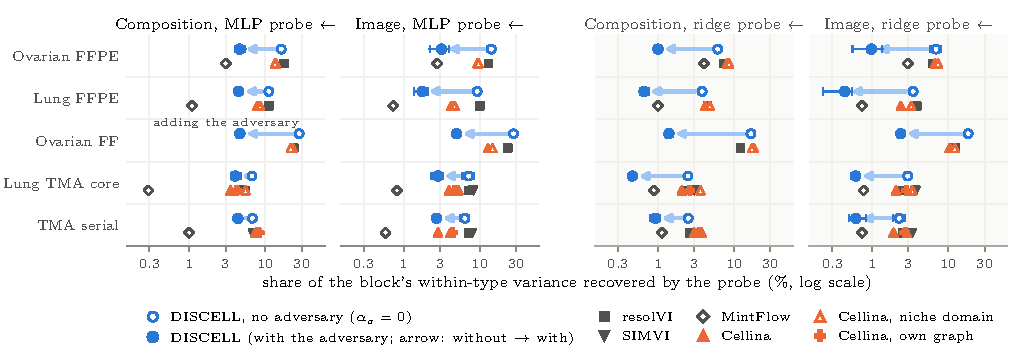
\includegraphics[width=\textwidth]{figures/fig_probe_data}
\caption{What the adversary removes from the intrinsic latent, per section. For each block and probe, the share of the block's within-type variance that the held-out probe explains from $\vz$ beyond the permutation floor ($1 - e^{-2\,\mathrm{excess}}$), in \% on a logarithmic scale: DISCELL without the adversary ($\alphaa = 0$, two seeds; open circle), with an arrow to DISCELL with it (the final fits, three seeds; filled circle), each with its range over seeds, and below them the comparison methods on the same section. The ridge probe (right, shaded) is the secondary read. Arrows point toward the better direction. On the serial section, the Cellina rows and MintFlow are the core's models transferred. SIMVI and MintFlow are absent on the sections where they could not be run (\cref{tab:baselines}). The values, and the fraction of the uncontrolled excess left, are in \cref{tab:probe}.}
\label{fig:probe-data}
\end{figure*}

\paragraph{The cell cycle.}
The cycle is an intrinsic state that the lineage labels do not encode, and it is carried by $\vz$ and not by $\vw$ (\cref{tab:headline,tab:headline-full}). The difference between the two holds at every leak fraction of the grid on every section, the serial section included (\cref{fig:breakdown-data}). A linear regression on the leading principal components of the counts explains less of the cycle scores than $\vz$ does on three sections, but more on the fresh-frozen section, the deepest ($83\%$ of their variance, against $74$ to $77\%$ for $\vz$). The cycle scores are not ground truth: they are gene-set scores of the cell's own segmented counts (\cref{app:readouts}), so transcripts leaked from cycling neighbours and expression induced by the environment raise them too, and the cycling set is chosen by them. That the response, close to its prior mean, a function of the neighbourhood (\cref{sec:results-w}), explains almost none of their within-type variance says that little of this axis follows the neighbourhood as the response represents it; it does not make the axis the cell's own, since $\vz$ is encoded from the same counts and would carry a leaked cycle signal, which the neighbours' types do not register. The sweep varies the leak fraction the model assumes, not the scores, so the asymmetry holding across it shows that the allocation does not depend on that assumption, not that the scores are free of leaked transcripts.

\paragraph{Merged subtypes.}
The lineage labels merge states and locations into their lineage, so the merged sublabels are held-out targets with a known allegiance: a state should be read from the intrinsic state, a location from the response (\cref{app:subtype}). On the primary section, where the sublabels are curated, the locations and two of the three tumour states follow it: the response, and equally its prior mean, separates tumour- from stroma-associated fibroblasts and endothelial cells (on two seeds of three by the pre-set call), and $\vz$ separates proliferating and inflammatory tumour cells (on every seed). The exceptions are states that also occupy a region, which both latents read: VEGFA$^+$ tumour cells on the primary section and three tumour-state clusters on the fresh-frozen section, while on the TMA core myofibroblasts among adventitial fibroblasts are read better from the response than from $\vz$. Merging such a state into its lineage moves part of it into the context regression, which is the cost of lineage labels anticipated in \cref{sec:setting,sec:invariance}.

\subsection{What the Response Carries}
\label{sec:results-w}
\readorder{7}
% manifest rows 6-8 (transport mean read, Read A, Read B), 14 (atlas, GO localisation), 15-17 (external criteria), 37 (held-out tiles)

\paragraph{Transport.}
\flag{TRIM}{about 450 words; Read A, twin margin and fold counts to app:response} \flag{REVIEWER}{keep the held-out-tiles read beside the headline read (decided 09-30)} The response is read through what the model predicts when a cell type is moved from one niche to another. For each type and pair of niches, the model's prediction holds the source cells' intrinsic state fixed and moves the prior mean of the response and the foreign influx to the target niche, and it is scored against the observed difference in the type's mean expression between the two niches, relative to the noise ceiling, the share of that difference that is reproducible between two random halves of the cells (\cref{app:readouts}). Over the panels whose ceiling is high enough to be read, the prediction recovers $0.65$ to $0.73$ of the ceiling (\cref{tab:headline}); its intervals (\cref{tab:headline-full}) have a coverage nearer $0.8$ than $0.95$ at the ceilings of real panels (\cref{app:readouts}). On the first seed, the response programmes alone recover $0.52$ to $0.64$ of the ceiling and the leakage alone $0.21$ to $0.39$ (\cref{tab:cellina-cf}); the two parts are not additive, but the programmes carry the larger share on every section. The full prediction's margin over the leakage alone holds across most of the sweep, but its margin over the programmes alone cannot be graded by it, so the sweep leaves open whether the leakage term adds to the prediction beyond the programmes (\cref{sec:results-sweep}). At the level of single cells, the decoded source cells, transported, close $0.70$ to $0.83$ of the gap, in maximum mean discrepancy, between the untransported cells and the target cells, each target cell decoded at its own posterior, where the target type's mean profile closes between $-1$ and $0.29$ (Read A, the median over panels); and for each target cell, the transported source cell nearest to it in $\vz$ is closer to the target's own decode than a random transported source cell, the median distance being $39$ to $46\%$ smaller (the twin margin). The transport reads are cross-fitted over spatial folds, but most of the scored cells lie in the model's training tiles. Scored on held-out tiles only, the fraction of the ceiling moves in both directions: in the trusted tier it lies above the published interval on $3$ of the $9$ fits with both reads, below it on $4$ and inside it on $2$, and over all panels above on $8$ of $11$, below on $2$ and inside on $1$; Read A is lower on held-out tiles on $11$ of $12$ fits, and the twin margin moves by at most $0.024$ (\cref{fig:transport-heldout}, \cref{tab:transport-heldout}). An in-sample advantage of the model would lower the held-out reads throughout; the fraction of the ceiling does not move that way, while Read A does. The held-out pool is also a quarter smaller, with fewer trusted panels. We keep the published read and report the other beside it.

\paragraph{Programmes.}
\flag{MOVE}{GO lean is descriptive and off-thread; one sentence here, rest in app:response} The response has two to five effective programmes per section, and the first is reproduced across seeds (\cref{tab:headline}, \cref{tab:breakdown-traj}). Its genes lean toward extracellular products and away from nuclear ones on the ovarian FFPE, lung and TMA sections, on every seed (rank-biserial effect $0.08$ to $0.22$ and $-0.12$ to $-0.19$), and toward plasma-membrane products on eight of those nine fits (\cref{app:response}). On the fresh-frozen section the extracellular lean fades from positive to null across the three seeds, so it is not a finding there. A lean toward secreted and membrane genes is also what a gene-specific leak would produce, which the sweep cannot separate (\cref{sec:generative}), so the lean is reported as a description, not as evidence of a response.

\paragraph{External criteria.}
\flag{MOVE}{criteria detail to app:response; keep the leakage-alone and not-specific caveats} Three criteria taken from other models' papers, two of them comparison methods here, are applied to our fits (\cref{app:response}). Ligand and receptor genes take a larger share of the between-niche shift than other genes in the leakage channel on every section and seed (rank-biserial effect $0.18$ to $0.28$), and also in the response channel on the ovarian FFPE, lung and TMA sections ($0.12$ to $0.18$); on the fresh-frozen section the response's lean is small ($0.01$ to $0.03$) and not significant in any seed by the per-seed rank test. The breakdown test is a different one, an interval for the mean over the three seeds of the difference in share, resampled over tiles; it excludes zero up to $\kappa = 0.1$ and not from $\kappa = 0.2$, where the lean breaks down (\cref{fig:breakdown-data}). The criterion that ligand--receptor genes respond more is thus reproduced by leakage alone on every section. The niche is read far more from the response than from the intrinsic state: by the same nearest-neighbour estimator as the guard of \cref{tab:headline}, on another sample of held-out cells and against its own within-type floors (\cref{app:response}), the response carries $0.41$ to $0.63$ nats of information about the niche and $\vz$ $0.06$ to $0.11$, on all four sections, the lung section included. On the primary section, the response's predicted shift of each gene follows the ordered bands of tumour density across the section more closely than it follows the in-plane coordinate least correlated with them (mean $|\tau|$ of $0.78$ to $0.81$ against $0.51$ to $0.56$), and the contrast holds across the leakage grid (\cref{fig:breakdown-data}). It holds in tumour cells and macrophages and fails in the merged fibroblast class, whose stromal half lies along the bands. The contrast is not specific to the response: predictions from the intrinsic state and from depth alone also follow the bands more than the false axis, with a lower true-axis $|\tau|$ ($0.57$ to $0.68$) but a difference of similar size.

\paragraph{The per-cell channel.}
\flag{KEEP-CORE}{thread point 4: per-cell channel closed by design, stated as a scoped result} At the operating point the response posterior stays at its prior: its own deviation adds one part in a thousand or less to held-out reconstruction (\cref{tab:recon-modes}), and its per-cell divergence, though spatially organised within a fit, ranks different cells in different seeds (\cref{app:kl-maps}). A simulated per-cell response, planted along the response programme in a tenth of one type's cells and unpredictable from the niche, is not detected by the rule fixed in advance at any strength up to twice the niche effect, and it is increasingly absorbed by the intrinsic state as it grows (\cref{app:planted-percell}, \cref{fig:planted-percell}). At $\alphaw = 0.1$ the per-cell channel is therefore closed by design, not by the data. On the ovarian FFPE, fresh-frozen and TMA sections the response and its prior mean also read the merged sublabels alike, within $0.07$ in AUC, with one exception on the TMA core (\cref{app:subtype}), so the response readouts above are readouts of the context regression $\mpsi(\vc_i, t_i)$ there (\cref{sec:objective}). On the lung section they are not only that: the response separates clusters within three lineages better than its prior mean does (AUC $0.67$ to $0.73$ against $0.55$ to $0.59$), although its own deviation adds as little to reconstruction as elsewhere. Lowering the weight opens the channel at a cost in agreement with type (\cref{app:sensitivity}).

\subsection{The Leakage Sweep}
\label{sec:results-sweep}
\readorder{5}
% manifest rows 9-10 (kappa sweep, kappa-survival), 11 and 21-23 (sensitivity), 18 (marker pairs), 38 (breakdown points)

Every section was refitted at each of the six leak fractions with three seeds. The claimed contrasts across the grid are drawn in \cref{fig:breakdown-data}; the diagnostics are drawn in \cref{fig:kappa-sweep} of the appendix, with their values in \cref{tab:kappa-sweep}. The diagnostics move smoothly along the grid: held-out reconstruction is nearly flat up to the operating point and falls beyond it, the mirror $R^2$ falls on every section, the cycle $R^2$ of $\vz$ stays within its seed range and that of $\vw$ near zero, and the response's information about the niche declines slowly. The response programmes survive the grid, their overlap with a reference fit at the operating point staying comparable to the overlap between seeds there (\cref{tab:breakdown-traj}). Magnitudes carry no breakdown point and are reported as trajectories (\cref{app:sweep}): the transport fraction of the ceiling is lower at $\kappa = 0$ than at the operating point, peaks between $\kappa = 0.05$ and $0.2$, and at $\kappa = 0.4$ is below its value at $\kappa = 0$ only on the primary section.

\begin{figure*}[t]
\centering
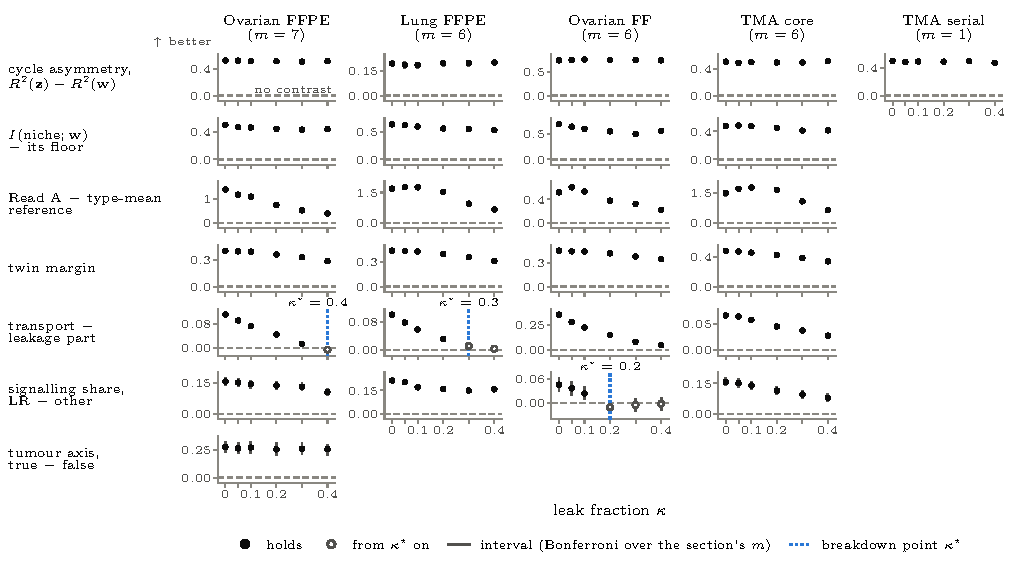
\includegraphics[width=\textwidth]{figures/fig_breakdown_data}
\caption{The claimed contrasts across the leakage sweep, the measured counterpart of \cref{fig:breakdown}. Rows: contrasts; columns: sections, with $m$ the number of contrasts in the section's set. At each $\kappa$, the mean over three seeds and its interval (spatial block bootstrap over tiles, two-sided, Bonferroni-adjusted over the section's $m$ contrasts); dashed, zero. Filled: the contrast holds at that grid point (every seed has its sign at $\kappa = 0$ and the interval excludes zero); hollow: from the breakdown point $\kappa^\star$ on (dotted). Each panel has its own vertical scale, which always includes zero, so an interval far from zero can be shorter than its marker. Arrows point toward the better direction: every contrast is signed so that it claims the side above zero. An empty panel: the contrast is not in that section's set. The transport prediction's margin over its programme part is not drawn: it is zero at $\kappa = 0$ by construction and is reported as a trajectory (\cref{tab:breakdown-traj}). The breakdown points are listed in \cref{tab:breakdown}.}
\label{fig:breakdown-data}
\end{figure*}

\paragraph{Breakdown points.}
Every claimed contrast holds at every leak fraction of the grid on every section, with two exceptions (\cref{fig:breakdown-data}, \cref{tab:breakdown}): the response's lean toward ligand--receptor genes on the fresh-frozen section, which breaks down at $\kappa = 0.2$, and the transported prediction's margin over its leakage part on the primary and lung sections, which breaks down in the upper half of the grid because a seed changes sign. The cycle asymmetry, the response's information about the niche, the two per-cell transport reads against their references and, on the primary section, the tumour-axis contrast are not explained away by leakage of the modelled form at any fraction up to $0.4$; leakage of another form is not ruled out (\cref{sec:sweep}). The transported prediction's margin over its programme part is a trajectory, not a claimed contrast: at $\kappa = 0$ no leakage is modelled, so the margin is zero by construction. Where a leak is modelled, the full prediction scores above its programme part in every seed on every section from $\kappa = 0.05$ to $0.2$; at the largest leak fractions it falls below it on the primary section and, in the mean, on the TMA core (\cref{tab:breakdown-traj}, \cref{app:sweep}).

\paragraph{Marker pairs.}
The marker-pair contrast is likewise a trajectory, of the decode (\cref{tab:breakdown-traj}). It compares the change in the rate at which mutually exclusive marker pairs are both detected in one cell, from the raw counts to the corrected decode, with the same change for control pairs that are expressed together (\cref{app:readouts}). It is negative at every grid value on the lung, fresh-frozen and TMA sections and positive on the ovarian FFPE section, and it is already present at $\kappa = 0$, where the decode removes no leakage; it therefore measures what decoding does to the counts, not what the leak correction removes, and is given no breakdown point. The correction's own effect at the operating point lowers exclusive and control double positives alike, although exclusive ones fall relative to control ones on every section, so the data do not show a removal specific to exclusive pairs (\cref{app:response}).

\paragraph{The form of the leak and other assumptions.}
Refitting the primary section with the leak's rate set per cell, from the neighbours' depth or density relative to the cell's own, or per gene at the same mean rate, moves no read by more than $1.3$ seed standard deviations of the final configuration (\cref{fig:sensitivity}; the values are in \cref{tab:sensitivity}). A fixed false-positive floor, a background rate per section, leaves the diagnostics in place but lowers the primary section's transport read from $0.65$ to $0.50$, a move of $8.3$ standard deviations and the largest of any arm, and less when the floor is scaled by cell area; on the TMA core it leaves transport in place. The transport read on the primary section is therefore sensitive to a background term the model does not have (\cref{app:sensitivity}).

\subsection{Comparison with Other Models}
\label{sec:results-baselines}
\readorder{4}
% manifest rows 4 and 34-36 (baseline battery, Cellina variants and counterfactual)

\Cref{fig:battery} scores every method by the same read-outs (the values are in \cref{tab:battery}), and \cref{fig:tradeoff} sets two of them against each other: how much within-type neighbour composition the intrinsic latent carries, by the probe of \cref{sec:invariance}, and how much within-type cell-cycle state it keeps. The comparison methods were fitted on our held-out cells as well (\cref{sec:setup}), so none of their reads is a held-out read. A DISCELL fit, its evaluations included, is up to $2.6$ times faster than the fastest competing model, Cellina, on three of the four sections, and slower than Cellina on the fresh-frozen section; it is over a hundred times faster than MintFlow wherever MintFlow could be run (\cref{tab:timing}).

\begin{figure*}[t]
\centering
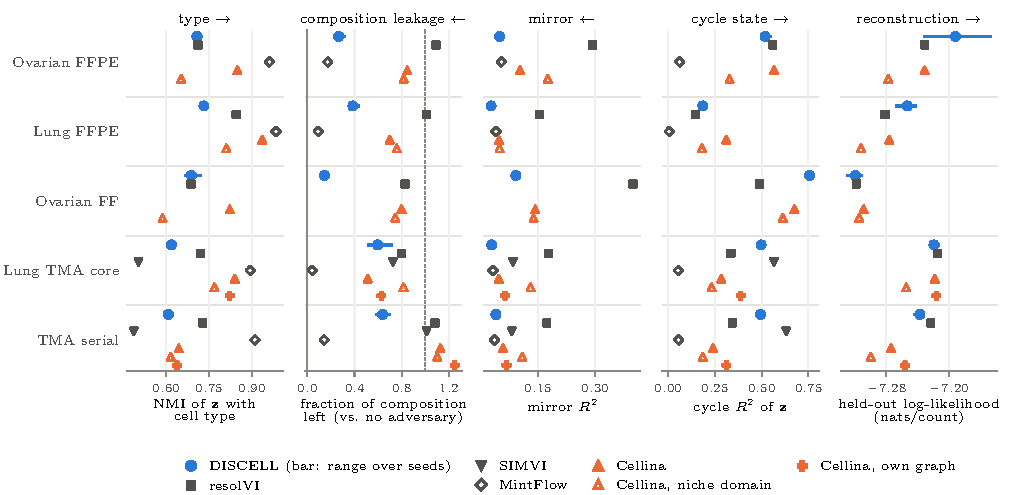
\includegraphics[width=\textwidth]{figures/fig_battery}
\caption{\flag{MOVE}{to app:baselines beside tab:battery; fig:tradeoff and fig:separation carry the thread} Every method on the same read-outs, at lineage labels, on the held-out cells of each section: NMI of the intrinsic latent with the type; the nonlinear probe's composition excess as a fraction of that of DISCELL without the adversary (solid at $0$, dashed at $1$); mirror $R^2$; cycle $R^2$ of the intrinsic latent on the top-decile cycling set; held-out reconstruction in nats per count. Markers as in \cref{fig:tradeoff}; DISCELL is the mean over three seeds with its range. Arrows point toward the better direction. The comparison methods are fitted on our held-out cells too, so their reads are not held-out reads. MintFlow's reconstruction is not reported, its stored value having been found invalid; refits are running (\cref{app:baselines}) \pending{MintFlow refits with the corrected export}, and SIMVI has no count decoder; methods are absent on the sections where they could not be run (\cref{tab:baselines}). The values are in \cref{tab:battery}.}
\label{fig:battery}
\end{figure*}

\begin{figure*}[t]
\centering
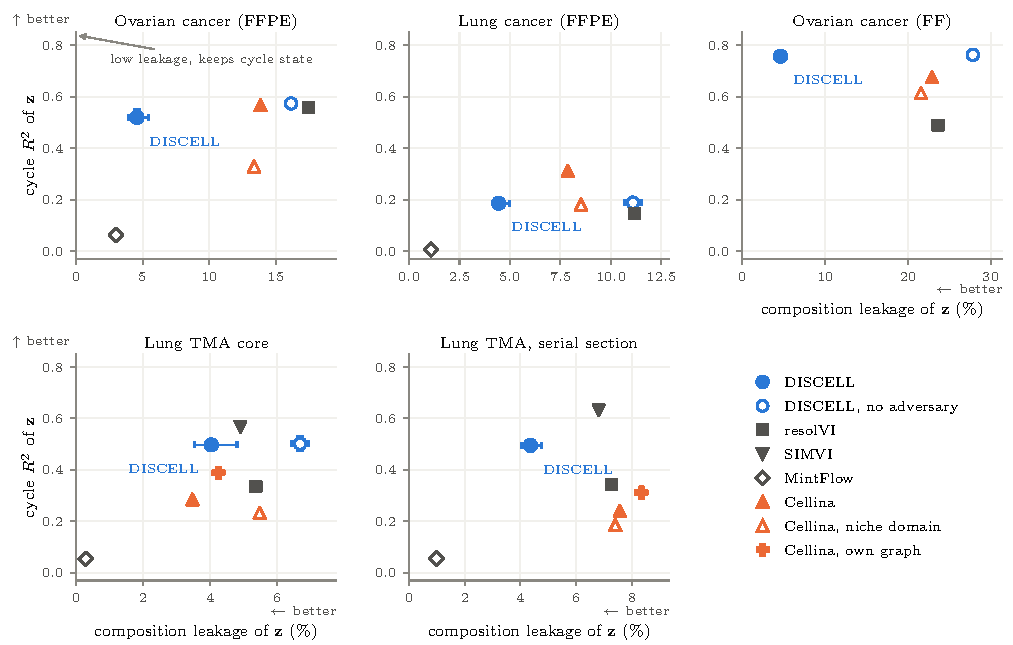
\includegraphics[width=\textwidth]{figures/fig_tradeoff}
\caption{\flag{KEEP-CORE}{thread point 4: less niche in z while keeping within-type state} Composition leakage of the intrinsic latent against the cell-cycle state it keeps, per section. \emph{Horizontal}: share of the within-type variance of neighbour composition that the held-out nonlinear probe explains from the intrinsic latent beyond the permutation floor ($1 - e^{-2\,\mathrm{excess}}$, in \%; \cref{tab:probe}). \emph{Vertical}: cycle $R^2$ of the intrinsic latent on the top-decile cycling set (\cref{tab:battery}). DISCELL: mean over three seeds, bars the range; open circle: DISCELL without the adversary (not read on the serial section). A method can be low on leakage by keeping little within-type state; DISCELL is low on leakage while keeping it. SIMVI and MintFlow are shown where their whole-section fits exist. Arrows point toward the better direction.}
\label{fig:tradeoff}
\end{figure*}

\begin{figure*}[t]
\centering
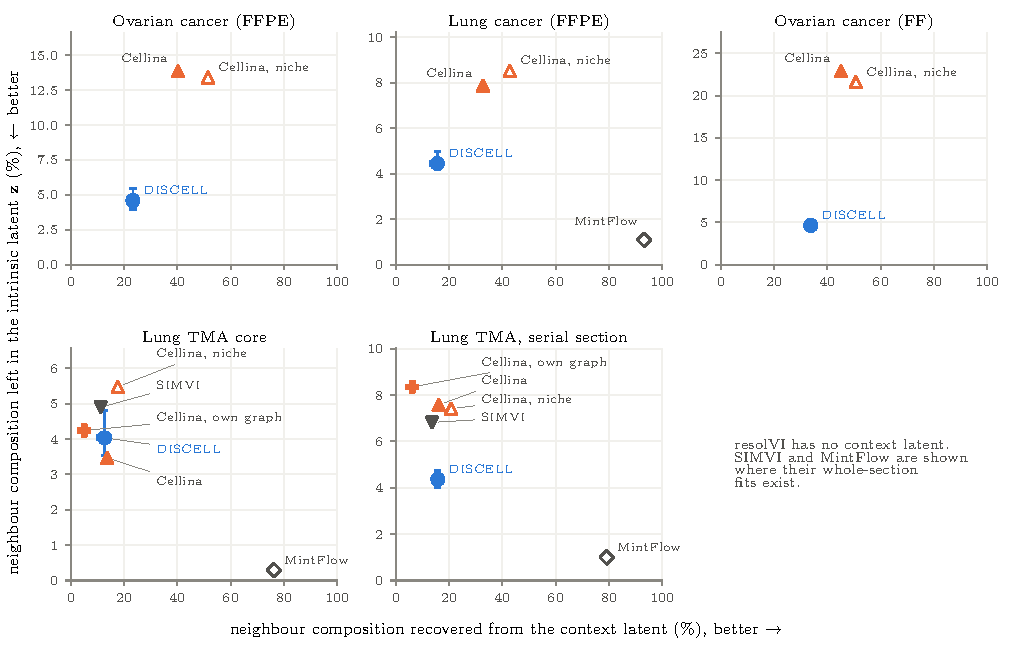
\includegraphics[width=\textwidth]{figures/fig_separation}
\caption{\flag{KEEP-CORE}{thread point 4: the context side graded like the intrinsic side} Neighbour composition in the context latent against the composition left in the intrinsic latent, per section. \emph{Horizontal}: share of the within-type variance of neighbour composition that the held-out nonlinear probe explains from each method's context latent beyond the permutation floor ($1 - e^{-2\,\mathrm{excess}}$, in \%; \cref{tab:context}). \emph{Vertical}: the same probe on the intrinsic latent, the horizontal axis of \cref{fig:tradeoff} (\cref{tab:probe}). A method that separates the two sits at the bottom right; arrows point toward the better direction. Markers as in \cref{fig:tradeoff}; DISCELL: mean over three seeds, bars the range. resolVI has no context latent; SIMVI and MintFlow are shown where their whole-section fits exist. MintFlow's intrinsic latent is close to a type label (\cref{tab:battery}).}
\label{fig:separation}
\end{figure*}

\paragraph{How to read the comparison.}
No single read-out ranks the methods; the pair in \cref{fig:tradeoff} does. On every section, each method that leaks less composition into its intrinsic latent than DISCELL keeps less cycle state (MintFlow, at a cycle $R^2$ of at most $0.06$; Cellina on the TMA core), and each that keeps more leaks more (Cellina on the FFPE sections, resolVI on the ovarian one, SIMVI on the TMA sections, narrowly on the core). DISCELL is never beaten on both, and is best on both on the fresh-frozen section; MintFlow is unbeaten too, but with almost no cycle state. DISCELL also has the lowest mirror $R^2$ on every section but the serial one (\cref{fig:battery}), though not the highest agreement with type.

\paragraph{Niche information in the intrinsic latent.}
\flag{REVIEWER}{keep the unfavourable rows: Cellina cycle, MintFlow residual, TMA core tie} On the ovarian FFPE, lung and fresh-frozen sections, DISCELL's intrinsic latent carries far less within-type neighbour composition than resolVI's or Cellina's, by both probes: the nonlinear probe recovers at most $5.5\%$ of its within-type variance, against $7.9$ to $24\%$ for the two comparison methods (\cref{tab:probe}). resolVI, with a single cell latent, serves as the reference of a model that does not separate the two. On the TMA core, where little leaks to begin with, the nonlinear residuals are close together and Cellina's is just below DISCELL's lowest seed, while the linear probe still finds several times less in DISCELL's latent than in resolVI's, Cellina's or SIMVI's; on the serial section only MintFlow's nonlinear residual is below DISCELL's. DISCELL keeps within-type state while doing so, although not the most of it everywhere (\cref{fig:tradeoff,tab:battery}): its cycle $R^2$ is the highest of all methods on the fresh-frozen section, while Cellina's is higher on the ovarian FFPE and lung sections, resolVI's on the ovarian FFPE section, and SIMVI's on the TMA core and its serial section, where SIMVI's latent also carries more composition. MintFlow reaches the lowest composition residuals of all, but its cycle $R^2$ is close to zero and its NMI with type high: its intrinsic latent is close to a type label. Cellina's NMI with type is higher than DISCELL's on every section, which its classifier on the intrinsic latent encourages, and its context latent mirrors its intrinsic latent more. Given our niche label as its domain, its best case on the probe, Cellina's adversary does not consistently lower its composition residual and lowers its NMI with type and its cycle $R^2$ on every section (\cref{app:baselines}).

\paragraph{Niche information in the context latent.}
Graded the other way, on each method's context latent (\cref{fig:separation,tab:context}), every context latent carries niche information beyond what the type carries. DISCELL's $\vmu_w$ holds less neighbour composition than Cellina's context latent on the ovarian FFPE, lung and fresh-frozen sections, about as much on the TMA core and its serial section, and far less than MintFlow's, which holds nearly all of it; it holds more of the image block than any comparison method's on the ovarian FFPE and lung sections, by both probes.

\paragraph{The counterfactual, head to head.}
Cellina also predicts expression under a rewired neighbourhood; scored by our transport reads on the same panels and draws, neither it nor DISCELL leads on every read (\cref{tab:cellina-cf}, \cref{app:cellina-cf}).

\section{CONCLUSION}
\label{sec:conclusion}

DISCELL writes a cell's counts as an intrinsic state, a response to its microenvironment and leakage from its neighbours, and makes explicit what the data leave open between the last two. The intrinsic state is pushed toward invariance to the niche given the cell's type, by architecture and by an adversary, and a held-out probe, independent of training, measures what remains: a few percent of the within-type variance of neighbour composition, less than competing models leave on most sections. The leakage enters through a fixed kernel on the section's own graph. The leak fraction is not estimated, since the data bound it only from above (\cref{prop:kappa-bound}), but swept, and every claimed spatial contrast is reported with the leak fraction at which it breaks down.

\paragraph{Limitations.}
Each is argued where it arises; they are collected here.
\begin{itemize}
\item \emph{The form of the leakage.} The leak fraction is one number per section, the leakage is the same for every gene and scales with the receiving cell's depth, and there is no ambient term (\cref{sec:generative}). A per-cell or per-gene variation in contamination is not covered by the sweep; its sensitivity to the leak's form is checked on the primary section only.
\item \emph{What the sweep separates.} It separates a spatial association from leakage of the modelled form, not from spatially organised intrinsic variation within a type, which the conditional invariance assigns to the response, nor from cells selecting their niche (\cref{sec:sweep}).
\item \emph{Labels.} The labels come from the same contaminated counts, and the decomposition is relative to their granularity: a state merged into its lineage becomes variation the model must place, and a spatially clustered state merged in this way is read as a response (\cref{sec:setting,sec:invariance}).
\item \emph{The invariance is incomplete.} With the adversary, a nonlinear probe still recovers $3.7$ to $5.8\%$ of the within-type variance of neighbour composition from the intrinsic state on every section; where little leaked to begin with, as on the TMA core, the adversary removes only $29$ to $48\%$ of what the uncontrolled model leaves. A probe at its floor bounds only the dependence it can detect (\cref{tab:probe}).
\item \emph{The response at the operating point.} With the response weight far above its bound-equivalent value, the response readouts are in effect readouts of the context regression; the per-cell channel is closed by design (\cref{sec:objective}).
\item \emph{Inference.} The intrinsic encoder does not see the foreign influx, so its posterior mean can differ from the exact one; in simulation the difference is close to that of an encoder that sees the influx, and on tissue it cannot be measured (\cref{app:planted}), and the posterior family is a compromise, so the uncertainty reported comes from the sweep and the seeds, not from the posterior (\cref{sec:inference}).
\item \emph{Identification.} Beyond the upper bound on the leak fraction and the invariance the probe grades, nothing guarantees that the intrinsic and response coordinates are identified (\cref{sec:sweep}).
\item \emph{Evaluation.} Cells of held-out tiles enter training as neighbours under a stop-gradient (\cref{sec:batching}), every fit is to one section, and only one section is held out whole. Two of the comparison methods have so far been run on only some of the sections (\cref{tab:timing}).
\end{itemize}

\paragraph{Future work.}
Three extensions follow directly. A perturbed and an unperturbed condition would add a third source of variation, so that the decomposition becomes intrinsic state, microenvironmental response and perturbation response, with the leakage sweep applied to all three. An operating point with an open per-cell response channel would support per-cell anomaly scores and counterfactuals with abduction. And a nuclear/extranuclear split of the transcripts would supply the gene a cell cannot express itself that the upper bound needs to become an estimate of the leak fraction (\cref{prop:kappa-bound}). Beyond the assay used here, the model needs counts assigned to segmented cells, one position per cell, a type label and an image descriptor; what that would require on other imaging platforms, on sequencing-based arrays and for protein imaging is discussed, untested, in \cref{app:inputs}.


\bibliographystyle{apalike}
\bibliography{references}

\section*{Checklist}

\todo{Answer at submission time. Questions must not be modified; the instruction paragraph of the template has been removed.}

\begin{enumerate}
\item For all models and algorithms presented, check if you include:
  \begin{enumerate}
  \item A clear description of the mathematical setting, assumptions, algorithm, and/or model. [Yes]
  \item An analysis of the properties and complexity (time, space, sample size) of any algorithm. [Yes]
  \item (Optional) Anonymized source code, with specification of all dependencies, including external libraries. [Yes]
  \end{enumerate}
\item For any theoretical claim, check if you include:
  \begin{enumerate}
  \item Statements of the full set of assumptions of all theoretical results. [Yes]
  \item Complete proofs of all theoretical results. [Yes]
  \item Clear explanations of any assumptions. [Yes]
  \end{enumerate}
\item For all figures and tables that present empirical results, check if you include:
  \begin{enumerate}
  \item The code, data, and instructions needed to reproduce the main experimental results (either in the supplemental material or as a URL). [Yes]
  \item All the training details (e.g., data splits, hyperparameters, how they were chosen). [Yes]
  \item A clear definition of the specific measure or statistics and error bars (e.g., with respect to the random seed after running experiments multiple times). [Yes]
  \item A description of the computing infrastructure used. (e.g., type of GPUs, internal cluster, or cloud provider). [Yes]
  \end{enumerate}
\item If you are using existing assets (e.g., code, data, models) or curating/releasing new assets, check if you include:
  \begin{enumerate}
  \item Citations of the creator If your work uses existing assets. [Yes]
  \item The license information of the assets, if applicable. [Yes]
  \item New assets either in the supplemental material or as a URL, if applicable. [Yes]
  \item Information about consent from data providers/curators. [Not Applicable]
  \item Discussion of sensible content if applicable, e.g., personally identifiable information or offensive content. [Not Applicable]
  \end{enumerate}
\item If you used crowdsourcing or conducted research with human subjects, check if you include:
  \begin{enumerate}
  \item The full text of instructions given to participants and screenshots. [Not Applicable]
  \item Descriptions of potential participant risks, with links to Institutional Review Board (IRB) approvals if applicable. [Not Applicable]
  \item The estimated hourly wage paid to participants and the total amount spent on participant compensation. [Not Applicable]
  \end{enumerate}
\end{enumerate}


\clearpage
\appendix
\thispagestyle{empty}
\onecolumn
\aistatstitle{DISCELL: Supplementary Materials}

\section{DERIVATIONS}
\label{app:derivations}
\readorder{21}

\subsection{The Reconstruction Bound}
\label{app:bound}

Fix a cell $i$ and hold $\vc_i$ and $\rhobar_i$ constant, as \cref{sec:batching} does; every probability in this appendix is conditional on $\rhobar_i$, which we suppress from the notation. Then
\begin{align}
  \log p(\vx_i \mid \vc_i, t_i)
  &= \log \iint p(\vx_i \mid \vz, \vw)\, p(\vw \mid \vc_i, t_i)\, p(\vz)\, d\vz\, d\vw \\
  &\geq \E_{q(\vz)\,q(\vw \mid \vz)}\Big[\log p(\vx_i \mid \vz, \vw) + \log p(\vw \mid \vc_i, t_i) + \log p(\vz) - \log q(\vz) - \log q(\vw \mid \vz)\Big] \label{eq:jensen}\\
  &= \E_{q(\vz)}\Big[\E_{q(\vw \mid \vz)}\big[\log p(\vx_i \mid \vz, \vw)\big] - \KL\big(q(\vw \mid \vz)\,\|\,p(\vw \mid \vc_i, t_i)\big)\Big] - \KL\big(q(\vz)\,\|\,p(\vz)\big),
\end{align}
where \cref{eq:jensen} is Jensen's inequality under the variational family $q(\vz)\,q(\vw \mid \vc_i, t_i, \vz, \vx_i)$. Because $q(\vw \mid \cdot)$ conditions on the sampled $\vz$, the exact bound keeps the $\vw$-divergence inside $\E_{q(\vz)}$. The divergence between two diagonal Gaussians is available in closed form,
\begin{equation}
  \KL\big(\N(\vmu, \vsigma^2)\,\|\,\N(\mathbf{m}, \mathbf{s}^2)\big) = \sum_k \Big[\log\frac{s_k}{\sigma_k} + \frac{\sigma_k^2 + (\mu_k - m_k)^2}{2 s_k^2} - \frac{1}{2}\Big],
  \label{eq:gauss-kl}
\end{equation}
and evaluating it at the single reparameterised draw of $\vz$ used for the reconstruction term is an unbiased one-sample estimate of $\E_{q(\vz)}[\KL(\cdot)]$.

Summed over cells, with each neighbour's $\vz_j, \vw_j$ drawn from its own posterior as in \cref{sec:batching}, $\sum_i L_i$ is a one-sample estimate of the evidence lower bound of the coupled model, $\log p(\{\vx_i\} \mid \{\vc_i, t_i\})$, under the fully factorised family $\prod_i q(\vz_i)\, q(\vw_i \mid \vz_i)$. The per-cell bounds are not independent terms, since $\rhobar_i$ is a function of the neighbours' latents. The stop-gradient removes the terms $i \ne j$ from the gradient with respect to $q_j$, so training ascends a partial gradient of this bound: a fixed-point iteration in which each step treats the current $\rhobar$ as data.

\subsection{The Intrinsic Path and the Factor \texorpdfstring{$(1+\omega)$}{(1+omega)}}
\label{app:pathb}

\flag{TRIM}{first paragraph repeats 2.4; keep the gap derivation and the Slavutsky contrast} A second bound on the same evidence holds by restricting the variational family to $q(\vw) := p(\vw \mid \vc_i, t_i)$, which zeroes the $\vw$-divergence and leaves
\begin{equation}
  \log p(\vx_i \mid \vc_i, t_i) \geq \E_{q(\vz)}\E_{p(\vw \mid \vc_i, t_i)}\big[\log p(\vx_i \mid \vz, \vw)\big] - \KL\big(q(\vz)\,\|\,p(\vz)\big) =: L_i^{z}.
\end{equation}
Call the bound of \cref{app:bound} $L_i$. Each carries its own $-\KL(q(\vz_i)\|p(\vz_i))$, so $L_i + \omega L_i^{z}$ contains $-(1+\omega)\KL(q(\vz_i)\|p(\vz_i))$. Omitting the second copy breaks the correspondence with $L_i + \omega L_i^{z}$ even at $\omega = 1$.

The construction mirrors the two-bound objective of \citet{slavutsky2025}, where the sum of the shared-only and joint bounds corresponds to minimising $\KL(q(\vz) \,\|\, p(\vz \mid \vx)) + \KL(q(\vz)q(\vw) \,\|\, p(\vz,\vw \mid \vx, u))$ with $u$ their condition label, a sum of two non-negative divergences. Here, unlike in \citet{slavutsky2025}, whose shared-only term decodes from $\vz$ alone and so bounds a different model, both terms bound the same evidence,
\begin{equation*}
  L_i + \omega L_i^{z} \le (1+\omega)\log p(\vx_i \mid \vc_i, t_i),
\end{equation*}
with gap $\KL\big(q(\vz)q(\vw \mid \vz)\,\|\,p(\vz,\vw \mid \vx_i,\vc_i,t_i)\big) + \omega\,\KL\big(q(\vz)p(\vw \mid \vc_i,t_i)\,\|\,p(\vz,\vw \mid \vx_i,\vc_i,t_i)\big)$. One $q(\vz)$ serves two variational families, so its optimum is a compromise and not the best approximation of the posterior under either, which is one of the reasons uncertainty is reported from the leakage sweep rather than from $q$. The invariance term sits outside the bound for a separate reason (\cref{app:posterior-reg}).

Why the intrinsic path is load-bearing: in \citet{slavutsky2025} the shared code is kept informative by a reconstruction from $\vz$ alone and by a prior on $\vw$ centred on the class-wise means of $\vz$. Our intrinsic path is the analogue of the first. We have no analogue of the second: our prior on $\vw$ never references $\vz$, and the prior on $\vz$ is a standard normal, so nothing else in the objective rewards $\vz$ for being informative. The intrinsic path supplies that pressure directly, since under it $\vz$ must explain the cell given only the expected response. It decodes through the same leakage mixture as the first term, at the same $\kappa$, so it never treats the counts as free of leakage and the two terms never disagree about how much of them is leakage. At the final configuration that pressure acts on the allocation more than on $\vz$ alone: without the path, $\vz$ keeps most of its type and cycle content, and $\vw$ takes up type signal (\cref{app:sensitivity}).

\subsection{The Invariance Term as Posterior Regularisation}
\label{app:posterior-reg}

\flag{MERGE}{repeats 2.5 nearly verbatim; fold the looser-sense clause into app:pathb} Neither $\Pen$ nor $\Adv_i$ is part of any bound. Both are posterior regularisation in the spirit of \citet{ganchev2010}: a constraint on the variational family, $\I(\vz; [\vy, \vPhi] \mid t) = 0$, written as a penalty on the variational objective. This is the same status \citet{slavutsky2025} give their adversarial term. It is a statement about which $q$ are admissible, not a modification of the generative model, which does not model $\vy$ or $\vPhi$ at all; the constraint states what the decomposition is meant to satisfy, and it acts on the aggregate of the encoder's outputs over cells rather than on each cell's posterior, so it is posterior regularisation in a looser sense than the per-instance expectation constraints of \citet{ganchev2010}.

\subsection{The Gaussian Conditional Mutual Information}
\label{app:gaussian-mi}

For jointly Gaussian $(\vz, \vv)$ with covariance $\Sig_{[\vz,\vv]}$ and marginal covariances $\Sig_{\vz}, \Sig_{\vv}$, the mutual information is $\I(\vz;\vv) = \tfrac12[\logdet\Sig_{\vz} + \logdet\Sig_{\vv} - \logdet\Sig_{[\vz,\vv]}]$ \citep{cover2006}. \cref{eq:penalty} applies this per type and averages with the type frequencies, which is the Gaussian estimate of $\I(\vz;\vv \mid t)$ under a type-wise Gaussian assumption. Two properties used in \cref{sec:invariance} follow directly. First, the value is invariant to a per-dimension rescaling $\vu \mapsto \mathbf{D}\vu$ with $\mathbf{D}$ diagonal: each log-determinant gains $\log\det$ of the corresponding block of $\mathbf{D}^2$, and the blocks of $\mathbf{D}$ for $\vz$ and $\vv$ together make up $\mathbf{D}$, so the three terms cancel exactly. The penalty may therefore be computed on correlation matrices. Second, on the simplex $\sum_k y_k = 1$ the covariance of the full composition vector is singular and the log-determinant is $-\infty$; dropping one column removes the constraint without changing the information, since the dropped column is a deterministic function of the others.

\subsection{Symmetries of the Response}
\label{app:symmetries}

\begin{proof}[Proof of \cref{prop:symmetries}]
Write $\mathbf{u}_i = a(\vz_i) + \vB\vw_i$ for the logits of \cref{eq:gen-rho}. The terms of $J$ that involve $a$, $\vB$, $\vw$ or $\mpsi$ are the two reconstruction terms, which are expectations of functions of the logits of cell $i$ and, through $\rhobar_i$, of its neighbours, and the prior divergence of $\vw$. The $\vz$-divergence and the invariance penalty depend only on $q(\vz_i)$ and $t_i$ and are untouched by all three maps.

(a) $\vB\mathbf{Q}^\top\mathbf{Q}\vw_i = \vB\vw_i$, so every draw has the same logits, hence the same $\vrho_i$, $\rhobar_i$ and $\vp_i$. Under the prior of \cref{eq:gen-w}, $\mathbf{Q}\vw_i \sim \N(\mathbf{Q}\mpsi, \sigma_w^2\mathbf{Q}\mathbf{Q}^\top) = \N(\mathbf{Q}\mpsi, \sigma_w^2\vI)$, which is the mapped prior, so the distribution of the counts is unchanged. In $J$, the mapped posterior and the mapped prior are the images of the originals under $\vw \mapsto \mathbf{Q}\vw$, so both reconstruction terms, the second of which draws $\wbreve_i$ from the prior, are unchanged, and the divergence between two distributions is invariant under a common bijection. For a signed permutation, $\mathbf{Q}\diag\boldsymbol{\nu}^2\mathbf{Q}^\top$ is the diagonal matrix with the entries of $\boldsymbol{\nu}^2$ permuted.

(b) The logits become $\mathbf{u}_i + \big(c(\vz_i) + \mathbf{b}^\top\vw_i\big)\mathbf{1}$, a shift by a scalar that is the same for every gene, and the softmax is invariant under such a shift. Every clean composition is therefore unchanged for every draw, and no other term of $J$ involves $a$ or $\vB$.

(c) For $\vz$ in the support of $q(\vz_i)$, $\tau(\vz) = t_i$, so the logits become $a(\vz) - \vB\boldsymbol{\delta}_{t_i} + \vB(\vw + \boldsymbol{\delta}_{t_i}) = a(\vz) + \vB\vw$, both for posterior draws, which are shifted with the posterior mean, and for prior draws $\wbreve_i$, which are shifted with $\mpsi$. The same holds for every neighbour, so $\rhobar_i$ is unchanged. The divergence between two Gaussians with the same covariances depends on their means only through their difference, and both means are shifted by $\boldsymbol{\delta}_{t_i}$.

Rescaling. With $\lambda_k = S_{kk}^2$, dimension $k$ of the divergence between $\N(\vmu_{w,i}, \diag\boldsymbol{\nu}_{w,i}^2)$ and $\N(\mpsi, \sigma_w^2\vI)$ changes under the map by $\tfrac12\big[(\lambda_k - 1)A_{ik} - \log\lambda_k\big]$ with $A_{ik} = \big(\nu_{w,ik}^2 + (\mu_{w,ik} - \psi_{ik})^2\big)/\sigma_w^2$, where $\psi_{ik}$ is coordinate $k$ of $\mpsi(\vc_i, t_i)$. Because $\sigma_w$ is fixed, for $\lambda_k \neq 1$ this vanishes only where $A_{ik} = \log\lambda_k/(\lambda_k - 1)$, not in general, so the map does not preserve $J$.

Readouts. Under (a) the differences $\vw_i - \bar\vw_t$ and $\mpsi(\vc_i, t_i) - \mpsi(\bar\vc_t, t_i)$ are multiplied by $\mathbf{Q}$ and $\vB$ by $\mathbf{Q}^\top$ on the right, so their products are unchanged. Under (b) each product gains $\mathbf{1}\mathbf{b}^\top(\cdot)$, a constant over genes, which centring removes. Under (c) both terms of each difference are shifted by the same $\boldsymbol{\delta}_t$, and the contexts are unchanged.
\end{proof}

\subsection{Feedback Amplification Through the Leakage Path (Heuristic)}
\label{app:amplification}

The following is a first-order heuristic, not a theorem. Write the decoder output of cell $j$ as $\vrho_j$ and suppose gradients were allowed to flow from cell $i$'s reconstruction through $\rhobar_i = \sum_j \beta_{ij}\vrho_j$ into the parameters that produce $\vrho_j$. Linearising around a fixed point of the coupled system, a perturbation $\delta$ of a cell's clean composition induces a perturbation $\kappa\,\beta\,\delta$ of its neighbours' fitted compositions, which feeds back through the same path; the total response is $\delta\sum_{n \ge 0}(\kappa \mathbf{P}_\beta)^n$ for a row-stochastic $\mathbf{P}_\beta$ built from $\beta$, whose spectral radius is at most one, so the geometric series is bounded by $1/(1-\kappa)$. The stop-gradient truncates the series at $n = 0$. The argument concerns perturbations of the fitted compositions; the gradient fixed point through shared decoder parameters is more involved, and we have not fitted the open-path model; \citet{ergen2025} close the same path for training stability.

\section{DESIGN RATIONALE}
\label{app:rationale}
\readorder{20}

This appendix carries the parts of the arguments of \cref{sec:method} that the main text only summarises. Some subsections, among them \cref{app:mirror,app:qw}, restate the main text's step before completing it.

\subsection{The Mirror Attractor}
\label{app:mirror}

The attention layer of \cref{eq:context-gat} computes logits $e_{ij} = \mathbf{a}^\top \mathrm{LeakyReLU}(\mathbf{W}_{\mathrm{dst}} \mathbf{h}_i + \mathbf{W}_{\mathrm{src}} \mathbf{h}_j)$ and aggregates $\sum_j \att_{ij} \mathbf{W}_{\mathrm{src}}\mathbf{h}_j$, so the destination feature $\mathbf{h}_i$ enters the \emph{attention} but never the \emph{value} \citep{brody2022}. With $\vz_i$ as the destination feature, the selection channel of \cref{sec:inference} opens. What the type query gives up is state-specific attention, which belongs in the decoder (as type-dependent loadings or a low-rank interaction with $\vz$) rather than in the context encoder.

\flag{MERGE}{repeats 2.3 and 2.7; keep the attention derivation above} The diagnostic is the within-type coefficient of determination of $\vz_i$ regressed on $\vc_i$ against a within-type permuted control (\cref{sec:selection}). The correlation between $\att_{ij}$ and $\simop(\vz_i,\vz_j)$ would serve under a $\vz$ query; with the type as query and types as sources the attention weights depend on the types alone (\cref{eq:context-closed}), and the correlation is vacuous. Downstream, a mirror is indistinguishable from ordinary posterior collapse of $\vw$; a free-bits remedy \citep{kingma2016} would mask it and leave the divergence uninterpretable, which is why the mirror is ruled out first.

Zeroing $\vz_i$ while keeping self-loops is not an alternative: the softmax still spends attention mass on the self-edge, down-weighting neighbours, and under $\vz \sim \N(\mathbf{0},\vI)$ the origin is the prior mean, so a zero vector asserts ``this cell is average'' rather than ``ignore this cell''.

\subsection{Why the Context Gets No Per-Edge Geometry, and Why the Graph Is Delaunay}
\label{app:graph}

\flag{TRIM}{four floats for one design choice; keep tab:contact and one figure} A discretised contact indicator (touching, near, far) looks as if it dodges the collinearity objection of \cref{sec:inference}, but on this platform, whose segmented polygons rarely touch, whether two of them touch is largely a measurement of local density: dense regions touch, sparse regions do not. The indicator would smuggle density back in, in the confounded direction, and a tolerance parameter only moves the threshold. \Cref{fig:graph-compare} shows it on one field: exact contact leaves most cells without a neighbour, a $1\um$ tolerance connects the dense tissue but leaves the separated cells of the sparse tissue isolated, and Delaunay adjacency connects them all.

\begin{figure}[t]
\centering
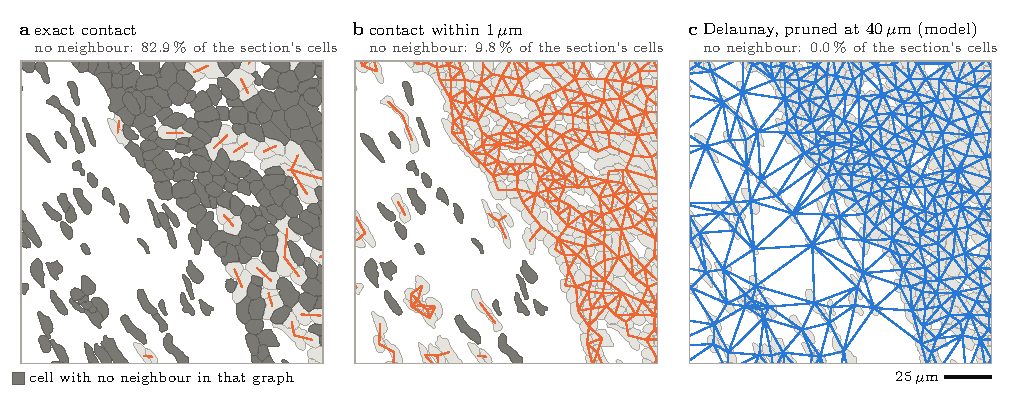
\includegraphics[width=\textwidth]{figures/fig_graph_compare}
\caption{Three neighbour graphs on one $160\um$ field of the primary section, each a subset of the model's edge set. \textbf{a},~Edges whose segmented polygons touch. \textbf{b},~Edges along which the two polygons run within $1\um$ of each other, the contact of \cref{tab:contact}. \textbf{c},~The model's graph: Delaunay adjacency pruned at $40\um$. Cells with no edge in a panel's graph are dark. The share above each panel is over the whole section, among cells with at least one edge in~c. The field is chosen to be representative: among fields that contain both sparse and dense tissue, it is the one whose shares under a and b are closest to the section's. Edges are drawn at one width; their weights in $\beta$ are illustrated in \cref{fig:overview}a. All panels share one scale.}
\label{fig:graph-compare}
\end{figure}

Delaunay adjacency resolves it: two cells are neighbours if and only if their Voronoi cells share a face, which is the correct notion of adjacency for a packing, built from centroids alone. The one parameter that returns is the pruning of long edges, and it is much less sensitive than choosing a neighbour count. The Voronoi face length is used in the kernel rather than shared segmented boundary because the Voronoi face is where the boundary between two cells effectively lies, its length is a contact-extent proxy defined whether or not the polygons touch, and it is independent of the expansion setting (\cref{fig:voronoi-face}).

\begin{figure}[t]
\centering
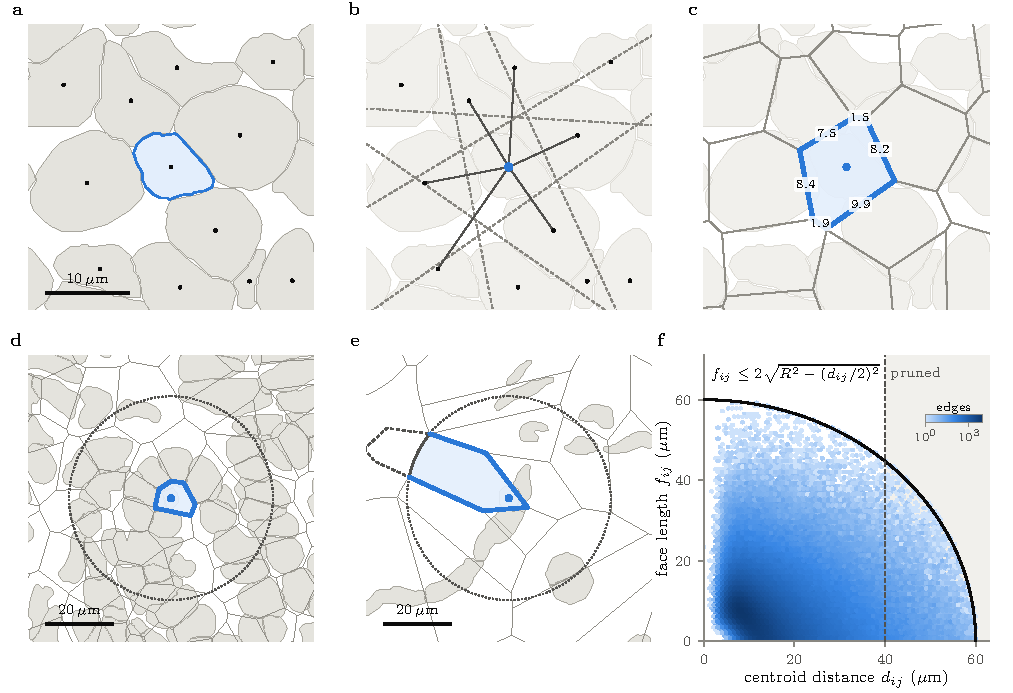
\includegraphics[width=\textwidth]{figures/fig_voronoi_face}
\caption{How the Voronoi face is built, and what bounds it, on the primary section. \textbf{a},~Segmented polygons and their centroids around a typical cell (blue). \textbf{b},~The polygons are set aside; each neighbour contributes the perpendicular bisector (dashed) of the segment joining the two centroids. \textbf{c},~The bisectors cut one another, and what survives between the cell and a neighbour is the face $f_{ij}$ (blue, length in $\mu$m); the shaded area is the cell's Voronoi region. Panels a--c share one scale. \textbf{d},~A dense neighbourhood and \textbf{e},~a cell at a tissue border, at one scale, each with the $30\um$ clip disc (dotted). At the border the unclipped region (dashed) runs into the gap, the disc bounds it, and the dark stretch of the outline between two faces is the clip arc. \textbf{f},~Face length against centroid distance for every edge of the section. Clipping bounds each face by the chord $2\sqrt{R^2-(d_{ij}/2)^2}$ of the disc, with $R = 30\um$, and removes every edge with $d_{ij} \ge 2R$; the model keeps edges up to $40\um$ (unshaded).}
\label{fig:voronoi-face}
\end{figure}

\Cref{tab:contact} and \cref{fig:contact-kernel} make the comparison concrete on every section. The sections were segmented mostly by an interior RNA stain rather than by nuclear expansion, and adjacent polygons still rarely touch. A contact kernel is therefore zero on about half of the edges, and it leaves a density-dependent share of cells with no leakage at all: up to a third of cells in the sparsest fifth of a section, almost none in the densest. Whether a cell can receive leakage would then be decided by local density, which is part of the niche. The Voronoi kernel gives every connected cell the same leak budget $\kappa$. Both kernels give nearer neighbours more weight; for $\beta$ that dependence is the one the distance decay introduces by design, and the face does not add to it.

\begin{table}[t]
\centering
\caption{Segmented-polygon contact as a leakage kernel, against the Voronoi-face kernel $\beta$, on every section and on the model's edge set (Delaunay adjacency pruned at $40\um$). Both kernels use the same distance decay $\exp(-d_{ij}/\tau)$ and the same row normalisation. The contact kernel weights an edge by the length of membrane along which the two segmented polygons run within $1\um$ of each other; $\beta$ weights it by the Voronoi face. FF: fresh frozen. \emph{Touching}: adjacent pairs whose polygons are at zero distance. \emph{No-leak cells}: connected cells whose kernel row is all zero, so that they receive no leakage at any $\kappa$; \emph{sparse} and \emph{dense} are the lowest and highest fifth of cells by the number of centroids within $20\um$. $\rho$: Spearman correlation, over edges, between a neighbour's share of the row and the gap between the two polygons. The Voronoi kernel has no zero-weight edges and no no-leak cells on any section. Its dependence on the gap is that of the distance decay alone (shares from the decay alone: $\rho$ between $-0.49$ and $-0.62$).}
\label{tab:contact}
\small
\setlength{\tabcolsep}{3.5pt}
\begin{tabular}{@{}lrrrrrrrrrr@{}}
\toprule
& \multicolumn{3}{c}{Segmented by (\% cells)} & \multicolumn{2}{c}{Edges (\%)} & \multicolumn{3}{c}{No-leak cells, contact (\%)} & \multicolumn{2}{c}{$\rho$(share, gap)} \\
\cmidrule(lr){2-4}\cmidrule(lr){5-6}\cmidrule(lr){7-9}\cmidrule(l){10-11}
Section & interior & boundary & nucleus & touching & no contact & all & sparse & dense & contact & $\beta$ \\
\midrule
Ovarian cancer (FFPE) & 69 & 29 & 2.0 & 3.5 & 47 & 9.8 & 33.6 & 0.6 & $-0.82$ & $-0.48$ \\
Lung cancer (FFPE) & 82 & 16 & 2.2 & 2.7 & 57 & 11.1 & 27.4 & 0.7 & $-0.84$ & $-0.55$ \\
Ovarian cancer (FF) & 70 & 28 & 2.5 & 6.7 & 38 & 3.2 & 10.6 & 0.1 & $-0.80$ & $-0.52$ \\
Lung TMA, section A & 87 & 12 & 1.0 & 2.2 & 47 & 6.3 & 24.8 & 0.1 & $-0.84$ & $-0.54$ \\
Lung TMA, section B & 87 & 12 & 1.2 & 2.2 & 47 & 6.2 & 24.6 & 0.1 & $-0.84$ & $-0.53$ \\
\bottomrule
\end{tabular}
\end{table}

\begin{figure}[t]
\centering
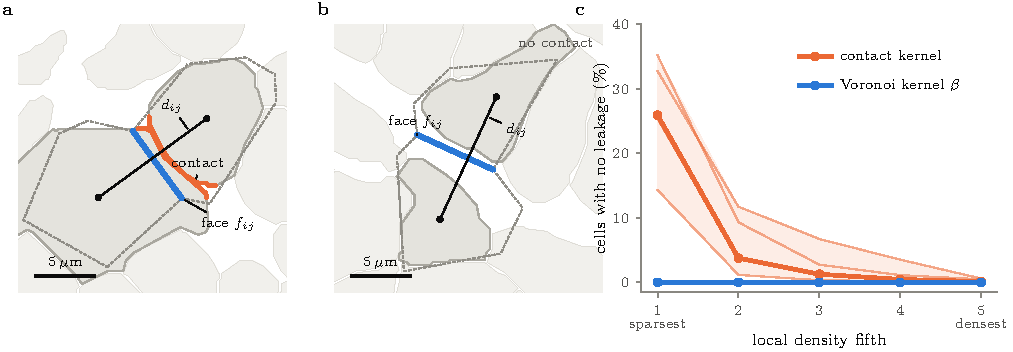
\includegraphics[width=\textwidth]{figures/fig_contact_kernel}
\caption{Why the leakage kernel is built on Voronoi faces rather than on segmented contact. \textbf{a},~An edge whose segmented polygons touch and \textbf{b},~an edge whose polygons do not, each the edge of its kind closest to the primary section's median centroid distance and median face length. The two have almost the same centroid distance $d_{ij}$ and face $f_{ij}$ (blue), which is all the kernel $\beta$ uses; contact (orange), the stretch of each cell's membrane within $1\um$ of the other cell, is present in a and absent in b. Dashed lines are the two cells' Voronoi regions; both panels share one scale. \textbf{c},~The share of cells that a contact-weighted kernel would leave with no leakage at all, by fifth of local density (centroids within $20\um$), on each section of \cref{tab:contact}: the median (bold), the range (band) and each section (thin). Both kernels use the model's edge set, the same distance decay and the same row normalisation; the Voronoi kernel leaves no connected cell without leakage on any section.}
\label{fig:contact-kernel}
\end{figure}


\flag{TRIM}{attention-sink test is development history, also in tab:deviations2; keep one} One consequence of the softmax over a Delaunay neighbourhood should be stated. With the type as query and one-hot types as sources, the logit of edge $ij$ depends on $(t_i, t_j)$ alone, say $s_{t_i t_j}$, and grouping the neighbours by type gives, per head,
\begin{equation}
  \mathbf{g}_i = \frac{\sum_k y_{ik}\, e^{s_{t_i k}}\, \mathbf{W}_{\mathrm{src}}\mathbf{e}_k}{\sum_k y_{ik}\, e^{s_{t_i k}}},
  \label{eq:context-closed}
\end{equation}
with $\mathbf{e}_k$ the $k$-th unit vector: a learned, type-specific reweighting of the neighbour composition in which the degree cancels. The context therefore depends on the fractions $\vy_i$, not on the counts. It distinguishes one tumour neighbour among six from five among six, but not a neighbourhood from the same neighbourhood with every type count scaled up together; in particular a single-type neighbourhood gives the same context whatever its size. On this tessellation the degree is nearly constant across the section, so a fraction determines a count and the blindness costs little. An attention sink, a fixed null logit that joins every softmax and restores a saturating dependence on the count, is implemented and was tested over three seeds. It learned no dose response, placing its half-point below a single neighbour, did not improve the held-out transport of the response, and in two of the seeds made the prior mean read the context less faithfully. It is therefore left off. It would become meaningful only on a graph whose degree varies, where the invariance target would have to grow with it.

\flag{CUT}{the edge-feature run was never done; cut, or run it and report} The fallback is empirical. If $\mpsi$ predicts responses poorly, or held-out reconstruction is worse than a comparison run whose attention layer carries edge features (distance, face length), that is direct evidence that the continuous signal mattered. If it is added back, the correlation between $\att_{ij}$ and $\beta_{ij}$ must be monitored: a high correlation means the attention has rediscovered the leakage kernel and $\vw$ is becoming collinear with $\rhobar$. That risk is tolerable while $\kappa$ is fixed, since there is no free contamination parameter to feed, and intolerable once $\kappa$ is estimated. \pending{the edge-feature comparison run has not been performed}

\subsection{The Image Descriptor and Its Mask}
\label{app:image}

\flag{TRIM}{the KRONOS vs KRONOS2 comparison can shrink to one sentence} The image descriptor $\vPhi_i$ is the embedding of a $128\um$ field around the cell ($256$ pixels at $0.5\um$ per pixel) in the section's four morphology channels (\cref{fig:overview}b), by KRONOS, a frozen foundation model for multiplexed tissue images \citep{kronos2025}: its first release, a ViT-S/16 with a $384$-dimensional embedding. The channels map onto the model's marker vocabulary only approximately: the membrane and $\alpha$SMA channels are antibody mixes read as their named component, and 18S RNA lies outside the vocabulary and is given an unused marker identity. The cell is removed by setting a disc around it to zero, not its own polygon: a polygon-shaped hole would keep the cell's outline, the most type-informative feature of all. The disc is centred on the crop anchor and has one radius for every cell, so the hole carries no information about the cell it removes, and it is filled with zeros, a constant artefact that the image model encodes identically for every cell. Its radius is the smallest that covers essentially every cell (\cref{fig:mask-radius}). A cell's covering radius, the radius of the smallest disc centred on its anchor that contains its polygon, has a long tail of elongated smooth-muscle cells; a $25\um$ disc leaves six cells of the primary section outside it and masks $12\%$ of the field. Those six cells were left out of the comparison below, and in the model their image descriptor is set to zero. A cell that sticks out of the disc would leak the identity the disc exists to remove, so partial coverage is not an option. At this density the disc also removes the cell's first ring or two, so $\vPhi_i$ describes the tissue beyond roughly $25\um$.

\begin{figure}[t]
\centering
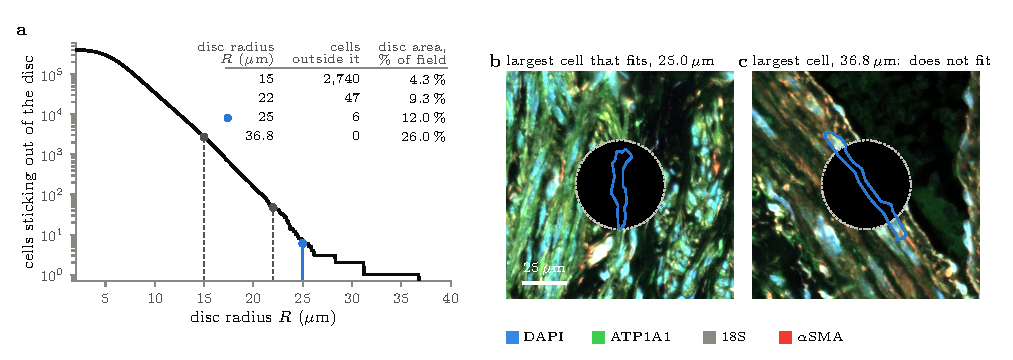
\includegraphics[width=\textwidth]{figures/fig_mask_radius}
\caption{Why the mask is a $25\um$ disc, on the primary section. \textbf{a},~The number of cells that would stick out of a disc of radius $R$ centred on the crop anchor, from each cell's covering radius; the table gives the radii considered, the cells left outside, and the share of the $128\um$ field each disc masks. The last row is the largest cell on the section. \textbf{b},~The largest cell that fits the chosen disc and \textbf{c},~the largest cell on the section, which does not, both drawn as the image model receives them: four channels, disc set to zero, with the cell's outline for reference. Both are elongated smooth-muscle cells.}
\label{fig:mask-radius}
\end{figure}

\Cref{tab:masking} shows what each mask leaves in the embedding, read by a multinomial logistic regression that predicts the cell's lineage label from it. The split is spatial, in tiles with a margin, because the fields of neighbouring cells overlap almost completely and a random split would put the same pixels on both sides. Three readings follow. The cell alone carries more type information than the whole patch: the surrounding tissue dilutes it rather than adding to it. Removing the cell costs little, because the patch embedding is dominated by its surroundings (\cref{fig:kronos-umap}a,~b). And the masked patch predicts the label less well than the neighbours' labels alone, so what it knows about the cell is what type-homogeneous neighbourhoods imply, which is what a descriptor of the niche should carry. On the masked patch the first release does at least as well as its successor KRONOS2 (a ViT-B/16 with a $768$-dimensional embedding, from the same authors); KRONOS2 is better only on the cell alone, where the model deliberately does not look. We therefore use the first release: its embedding is half as wide ($384$ against $768$ dimensions), which keeps the image part of the context descriptor small, and it embeds cells about five times faster.

\begin{table}[t]
\centering
\caption{What each mask leaves in the image embedding, on the primary section: macro one-versus-rest AUC of a multinomial logistic regression predicting the cell's lineage label (the labels the model is fitted with; 11 classes, Unassigned cells excluded as targets but counted as neighbours) from the embedding, on a spatial split ($1\,$mm tiles, cells within half a field of a tile edge dropped; $40{,}000$ training and about $74{,}000$ test cells), for the two releases of the image model, KRONOS and KRONOS2 \citep{kronos2025}. The first row predicts the label from the neighbours' labels alone, with no image. The model uses KRONOS with the disc zeroed (bold).}
\label{tab:masking}
\small
\begin{tabular}{@{}lcc@{}}
\toprule
Input to the classifier & KRONOS & KRONOS2 \\
\midrule
Neighbours' labels, no image & \multicolumn{2}{c}{$0.918$} \\
Whole patch & $0.881$ & $0.878$ \\
Disc over the cell zeroed & $\mathbf{0.857}$ & $0.846$ \\
The cell alone & $0.905$ & $0.919$ \\
The cell alone, native resolution & $0.923$ & -- \\
\bottomrule
\end{tabular}
\end{table}

\begin{figure}[t]
\centering
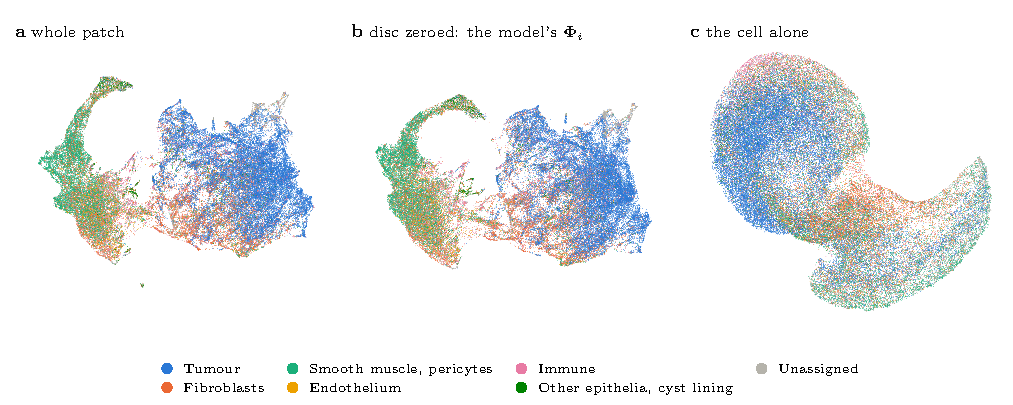
\includegraphics[width=\textwidth]{figures/fig_kronos_umap}
\caption{\flag{CUT}{adds little beyond tab:masking} The KRONOS embedding (first release, the one the model uses) under three masks, as UMAPs of the same $60{,}000$ cells of the primary section (principal components, then UMAP). \textbf{a},~The whole $128\um$ patch. \textbf{b},~The disc over the cell zeroed, the descriptor $\vPhi_i$ the model uses; it differs little from~a, because the patch is dominated by the surrounding tissue. \textbf{c},~Everything outside the cell's polygon zeroed, what the cell alone carries. Colour is the section's lineage label, the one the model is fitted with, with the smaller lineages grouped for display. Unassigned includes a low-depth class of mixed lineage that the section's original annotation had called a tumour subtype.}
\label{fig:kronos-umap}
\end{figure}

\subsection{Three Routes to a Vanishing Response Divergence}
\label{app:qw}

\flag{MERGE}{table repeats diagnostic (ii) of 2.7; fold into that sentence} \begin{center}
\begin{tabular}{@{}>{\raggedright\arraybackslash}p{0.2\textwidth}>{\raggedright\arraybackslash}p{0.4\textwidth}>{\raggedright\arraybackslash}p{0.34\textwidth}@{}}
\toprule
Cause & Check & Fix \\
\midrule
Posterior collapse & $\alphaw$ large relative to reconstruction & lower $\alphaw$; free bits \\
Mirror & within-type $R^2$ of $\vz_i$ on $\vc_i$ vs.\ permuted control & type embedding as query; types only as sources \\
Starved of ego evidence & does the response posterior receive $\vx_i$ directly? & add the direct path \\
\bottomrule
\end{tabular}
\end{center}

\subsection{Conditional Invariance and Label Granularity}
\label{app:conditional}

\flag{CHECK}{todo still open: the numbers are in DisCoVR's Table 19 (checked 09-23) but not quoted in the manuscript or devlog, so this needs a read of that table; the four-reasons list overlaps 2.1 and 2.5} The marginal-invariance failure is documented by \citet{slavutsky2025} for the conditional subspace VAE \citep{klys2018}, whose invariance drives the agreement between the shared code and the nuisance variable to zero while collapsing its agreement with cell type \todo{quote the exact numbers from that comparison}. Lineage-level labels are preferable to finer or state-defined ones for four reasons: fine labels leave $\vz$ with nothing to carry, they block more of the position$\to$fate$\to$expression path, they destroy the overlap that any conditional comparison needs, and, because $t_i$ is itself a function of $\vx_i$, hence of leakage and of any response that moves a cell across a label boundary, conditioning on it conditions on a descendant of the niche, so that even the true intrinsic state can depend on $\vy_i$ given $t_i$ near label boundaries \citep{hernan2004}.

\subsection{The Leak Fraction: Grid Range and Upgrade Path}
\label{app:kappa}

The grid runs from zero, the nested no-correction null, to $0.4$. On this platform a typical cell carries misassigned transcripts of about a tenth of its counts, and heavily contaminated cells are rare \citep{yang2025mistic}. The operating point $\kappa = 0.1$ (\cref{sec:setup}) matches that typical value, and the top of the grid is deliberately conservative, several times it.

This version of the model sweeps $\kappa$; it cannot estimate it. Assigning transcripts to cells by position does not settle it either: counts of transcripts that lie nearer a neighbour's nucleus than the cell's own are dominated by segmentation geometry, since a large cell beside small ones counts its own far-side transcripts as foreign, so such counts bound leakage from above but do not identify how it scales with the depth of the receiving or the donating cell. Estimation needs two views of one cell that share a foreign profile at different contamination levels, which a nuclear/extranuclear split of the transcript coordinates provides. Its identifying condition is that gene-wise nuclear retention varies across genes, which is also a reason to expect the gene-specific leakage that the main model does not represent (\cref{sec:generative}), and which a two-view likelihood would be the natural place to model; with constant retention both views lie on the same line between $\vrho_i$ and $\rhobar_i$ and nothing is pinned. Adding it does not restructure the model: the likelihood becomes a multinomial over $2G$ bins and $\kappa$ moves from hyperparameter to latent. We leave it as future work.

What the data say about $\kappa$ can be stated exactly at the level of compositions.

\Cref{prop:kappa-bound} (\cref{sec:sweep}) states it; the proof follows.
\begin{proof}[Proof of \cref{prop:kappa-bound}]
The clean composition implied by $\kappa'$ is $\vrho_i(\kappa') = (\vp_i - \kappa'\rhobar_i)/(1-\kappa')$, which sums to one for every $\kappa'$ and is non-negative in gene $g$ if and only if $\kappa'\bar\rho_{ig} \le p_{ig}$; this holds for every gene if and only if $\kappa' \le \bar\kappa_i$. Since $p_{ig}/\bar\rho_{ig} = \kappa + (1-\kappa)\rho_{ig}/\bar\rho_{ig} \ge \kappa$, the true value lies below the bound, and meets it exactly when a gene the neighbours express has zero share in the cell's own composition.
\end{proof}

The data therefore bound $\kappa$ from above and never from below, and a section-wide $\kappa$ must respect the bound of every cell. They pin it only through a gene the cell cannot express itself, such as a marker that an external atlas excludes for the cell's type, or through a second view of the cell such as a nuclear/extranuclear split. \Cref{fig:kappa-bound} draws both cases. The statement is about compositions: with counts the bound is soft, since a $\kappa$ above it charges each cell for neighbour transcripts it does not show, and the decoder's form can narrow the interval further, which is the route that expected low-dimensionality takes and that a response to the niche weakens (\cref{sec:intro}).

\begin{figure}[t]
\centering
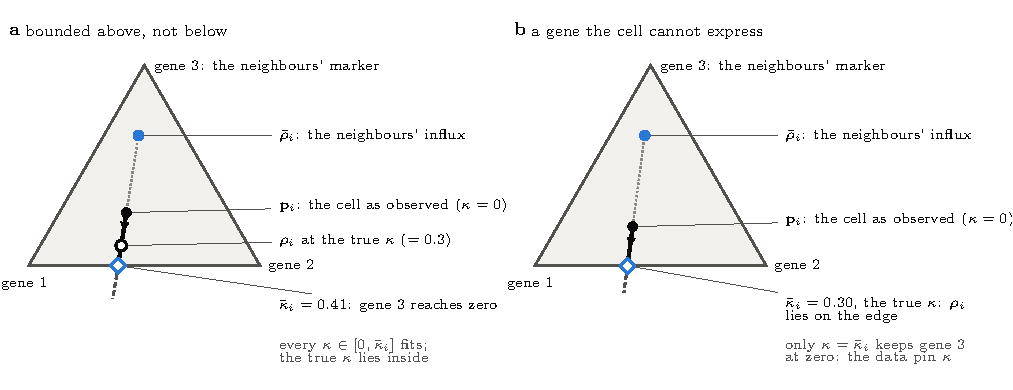
\includegraphics[width=\textwidth]{figures/fig_kappa_bound}
\caption{What the data say about $\kappa$, on the simplex of three genes; schematic, with compositions chosen for legibility. With the neighbours' influx $\rhobar_i$ held fixed, each $\kappa$ implies the clean composition $\vrho_i(\kappa) = (\vp_i - \kappa\rhobar_i)/(1-\kappa)$: a line that starts at the observed composition $\vp_i$ ($\kappa = 0$) and runs away from $\rhobar_i$ (arrow). It is valid until it leaves the simplex at $\bar\kappa_i$ (diamond) and invalid beyond (dashed). \textbf{a},~A cell that expresses a little of the neighbours' marker itself: every $\kappa \in [0, \bar\kappa_i]$ reproduces $\vp_i$ exactly, and the true value lies inside. \textbf{b},~A cell that cannot express the marker: its true composition lies on the edge, the line leaves the simplex exactly there, and $\bar\kappa_i$ is the true $\kappa$.}
\label{fig:kappa-bound}
\end{figure}

\flag{TRIM}{repeats def:breakdown and the fig:breakdown caption; keep the fibroblast example} \Cref{def:breakdown} is easiest to read on an example. A readout is any number reported from a fit, for instance how much a fibroblast programme differs between fibroblasts next to tumour and fibroblasts in stroma. At $\kappa = 0$ the model assigns all of that difference to the cells themselves. Refitting at each larger $\kappa$ attributes more of the resemblance between neighbours to leakage, so a difference that is only leakage shrinks toward its null value, and one that reflects biology persists. The breakdown point $\kappa^\star$ is the smallest leak fraction at which the readout can no longer be told from its null, or changes sign: how much leakage it would take to explain the readout away. \Cref{fig:breakdown} shows the four cases. A readout that survives every grid value cannot be explained by leakage of the modelled form up to the top of the grid (a). A contrast may shrink as $\kappa$ grows without breaking down (b): readouts shrink by construction, because the mixture takes over part of the resemblance between neighbours, and the contrast stands as long as its interval stays clear of zero. A readout that breaks down inside the grid is explained away by that much leakage (c), and one that breaks down at the first grid point above zero is explained away by any leakage at all (d). The higher the breakdown point, the stronger the finding. Read with \cref{fig:kappa-bound}, the two say what a finding would need: the data bound the leak fraction from above, so a readout whose breakdown point lay above that bound would survive every leak fraction the data allow. That bound is not computed on the sections here (\cref{prop:kappa-bound}), so what the grid supports is the weaker statement that a readout surviving it survives every leak fraction up to $0.4$.

\begin{figure}[t]
\centering
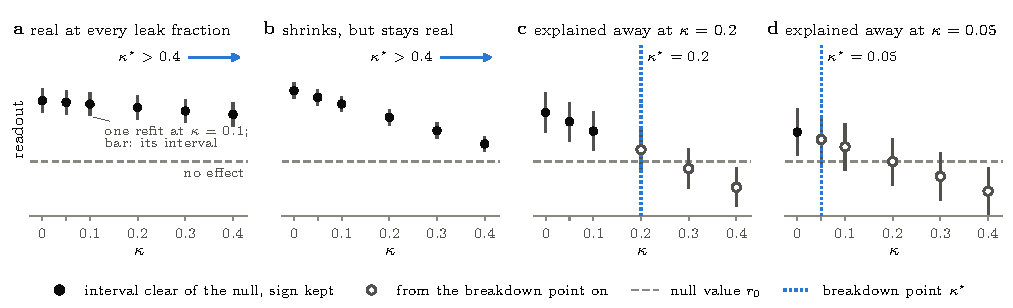
\includegraphics[width=\textwidth]{figures/fig_breakdown}
\caption{The breakdown point of \cref{def:breakdown}, on four schematic readouts: four different candidate findings, not four ways of choosing $\kappa$, which is never chosen. The curves are illustrative, not fitted, and only the grid of $\kappa$ is the model's. Each panel shows a readout at every grid value with its interval (bars) and its null value $r_0$ (dashed). Filled markers: the interval is clear of the null and the readout keeps the sign it has at $\kappa = 0$; hollow markers: from the breakdown point $\kappa^\star$ (dotted) on. Each point is a separate fit at that $\kappa$. \textbf{a},~A signed contrast that survives the grid, reported as $\kappa^\star > 0.4$. \textbf{b},~A contrast that shrinks as $\kappa$ grows, as expected by construction because more of the resemblance between neighbours is assigned to the mixture, but stays clear of zero: it also survives. \textbf{c},~A contrast that $20\%$ leakage explains away, $\kappa^\star = 0.2$; its sign flips beyond it. \textbf{d},~A contrast that breaks down at the first grid point above zero, $\kappa^\star = 0.05$: any leakage explains it away, so it is not separable from leakage of the modelled form.}
\label{fig:breakdown}
\end{figure}

\subsection{Learned Variances: What to Learn and What Not To}
\label{app:variances}

If a conditional $\sigma_w(\vc, t)$ is wanted, because it would standardise deviation against local variability so that a deviation of two in a niche where everyone deviates by two does not read as anomalous, it must be bounded, e.g.\ $\sigma_w \in [0.5, 2]$ through a scaled sigmoid, so that it cannot inflate away, and its mean over cells must be checked for upward drift over training.

The prior on $\vz$ is a standard normal. A richer prior, a mixture with one component per type or a VampPrior with archetypal pseudo-inputs \citep{tomczak2018}, would be a genuine upgrade for cell-type structure and would make $t$ a latent rather than an input, but that is a different change, not a variance question.

\section{IMPLEMENTATION DETAILS}
\label{app:implementation}

\subsection{Architecture and Hyperparameters}
\label{app:architecture}

\cref{tab:architecture} lists every network and every fixed quantity as implemented; the weights marked calibrated are set per section by the protocol of \cref{sec:invariance} and are not quoted here. All multilayer perceptrons use rectified-linear hidden units.

\begin{table}[t]
\centering
\caption{Networks and fixed quantities. $G$ genes, $K$ types, $\dPhi$ image-embedding dimension.}
\label{tab:architecture}
\small
\begin{tabular}{@{}p{0.2\textwidth}p{0.27\textwidth}p{0.48\textwidth}@{}}
\toprule
Component & Input & Layers / value \\
\midrule
Count encoding & $\vx_i$ & $[\log(1 + \vx_i \tilde\ell/\ell_i),\ \log\ell_i]$, $\tilde\ell$ the median total \\
$q(\vz_i \mid \vx_i, t_i)$ & count encoding $\oplus \onehot(t_i)$ & $256 \to 256 \to 2\dz$, $\dz = 20$ \\
Type query $\embed(t_i)$ & $t_i$ & learned table, width $K$ \\
Attention sources & neighbour $j$ & $\onehot(t_j)$, width $K$; an earlier version appended the neighbour's posterior mean under a stop-gradient and was dropped after a three-seed ablation \\
Attention layer & sources, query & one bipartite GATv2 layer, $4$ heads $\times\, 32$, averaged, LeakyReLU slope $0.2$, no self-loops, no edge features \\
Context $\vc_i$ & & attention output ($32$) $\oplus\ \vPhi_i$ ($\dPhi = 384$) $\oplus$ isolation flag ($1$) \\
Prior mean $\mpsi(\vc_i, t_i)$ & $\vc_i \oplus \onehot(t_i)$ & $64 \to \dw$, $\dw = 6$ \\
$q(\vw_i \mid \cdot)$ & $\vc_i \oplus \onehot(t_i) \oplus \vz_i \oplus$ count encoding & $256 \to 2\dw$ \\
Decoder $a(\vz_i)$ & $\vz_i$ & $256 \to G$ \\
Loadings $\vB$ & $\vw_i$ & linear $\dw \to G$, no bias \\
Adversary heads & $\vmu_{z,i} \oplus \onehot(t_i)$ & two heads $64 \to 64 \to K$ (composition) and $\to \Ephi = K$ (image niche) \\
Image niche $\ephi_i$ & $12$ principal components of $\vPhi$ & soft $k$-means memberships $\softmax(-d^2/T)$, $T$ the median nearest squared distance; the projection is fitted on a $50{,}000$-cell random subsample and applied to all cells, the $k$-means (four restarts) on all cells; fitted once and frozen \\
Invariance block $\vv_i$ & & $[\vy_i^{(-K)},\ 12 \text{ principal components of } \vPhi_i]$ \\
Held-out probes & $\vmu_{z,i} \oplus \onehot(t_i)$ & ridge regression ($\lambda = 10^{-3}$) and perceptron $64 \to 64$ ($300$ Adam steps at $10^{-3}$, batches of $2{,}048$), each scored per block against its own within-type permutation floor; both fitted on at most $30{,}000$ training-tile cells \\
\midrule
Graph & & Delaunay adjacency; Voronoi faces measured within $30\um$ discs; prune at $40\um$ \\
Kernel $\beta$ & & $f_{ij}\exp(-d_{ij}/\tau)$, $\tau = 20\um$, row-normalised over in-edges \\
Prior scale $\sigma_w$ & & $1$ (fixed) \\
\midrule
Leak fraction $\kappa$ & & swept over $\{0, 0.05, 0.1, 0.2, 0.3, 0.4\}$; the operating point $0.1$ is a grid point chosen on the primary section (\cref{sec:setup}) \\
$\omega$ & & $1$ \\
$\alphaz$ & & $\tfrac12/\lbar$, half the bound-equivalent value, with $\lbar$ the section's count scale (\cref{sec:objective}) \\
$\alphaw$ & & $0.1$, far above $1/\lbar$ (\cref{sec:objective}); ramped linearly from $0$ over the first $30$ epochs \\
$\alphaa$ (adversary) & & $0.3$; six head updates per model update at learning rate $2 \times 10^{-3}$, set so that the independent probe, not the heads' own loss, certifies head strength; composition half weighted $\lambda_y = 3$ \\
$\alphaa$ (closed form) & & calibrated by the same probe protocol \\
Moving-average rate, shrinkage & & $0.05$, $0.05$; support floor $10\times$ joint dimension \\
\midrule
Tiles & & recursive median split into rectangles of $\leq 4{,}096$ cells; $15\%$ of tiles held out \\
Optimiser & & Adam \citep{kingma2015adam}, learning rate $10^{-3}$, cosine annealing \citep{loshchilov2017} over the epoch budget, gradient-norm clip $10$ \\
Evaluation & & every $5$ epochs on posterior means; checkpoint accepted if held-out reconstruction improves and $\vz$--type agreement $\geq 0.9\times$ its running maximum; patience in epochs set with the budget; $\alphaw$ ramped linearly from $0$ over the first $30$ epochs, during which no checkpoint is accepted and patience does not count \\
Hardware & & one NVIDIA GeForce RTX 4090 (24\,GB) per fit \\
\bottomrule
\end{tabular}
\end{table}

\subsection{Choices Made in Implementation}
\label{app:deviations}

Where the model description of \cref{sec:method} leaves a choice open, \cref{tab:deviations} records what was done and why. Every entry is also stated in the method text; the table collects them in one place. \todo{author to decide whether this table stays; it duplicates the method text}

\begin{table}[t]
\centering
\caption{Implementation choices and their reasons.}
\label{tab:deviations}
\small
\begin{tabular}{@{}p{0.22\textwidth}p{0.36\textwidth}p{0.36\textwidth}@{}}
\toprule
Where & Decision & Reason \\
\midrule
Type input to $q(\vw)$ and $\mpsi$ & one-hot everywhere the type is an input; the learned type embedding exists only as the attention query, sized to match the source features & the query stands in for the $\vz_i$ that the cell deliberately does not contribute to its own context \\
Counts input to $q(\vw)$ & the same encoding as $q(\vz)$ & one encoding of the counts for both posteriors \\
Neighbour responses $\vw_j$ & a posterior draw from the same batched pass, under a stop-gradient & the neighbours' clean compositions must include their local programme (\cref{sec:batching}) \\
Invariance block & one composition column dropped & the simplex makes the full block singular; the information is unchanged (\cref{app:gaussian-mi}) \\
Penalty matrices & correlation rather than covariance form, plus $10^{-5}\vI$ on the correlation matrix before the log-determinant & identical value by scale invariance; bounded gradient; on a unit-diagonal matrix the additive term is a uniform relative jitter, not a variance-inflating ridge \\
Penalty gradient & straight-through: value from the moving averages, gradient from the batch & otherwise the effective strength of $\alphaa$ scales with the averaging rate \\
Penalty, adversary and probe input & posterior means $\vmu_z$, not samples & encoder noise would dilute the measured dependence \\
Objective granularity & per-cell mean over the batch rather than a sum & invariant to tile size \\
Evaluation draws & posterior means & the stopping signal should not ride reparameterisation noise \\
Image embedding dimension & the full native embedding into $\vc_i$ rather than a $32$--$64$-dimensional projection & the deciding test is held-out reconstruction with and without the projection; the invariance block uses $12$ principal components regardless \\
Probe target for the image & Gaussian log-likelihood gain on the continuous components, per block, rather than categorical cross-entropy against image-niche clusters & the closed-form penalty takes continuous components directly; a small nonlinear probe is fitted alongside and is the probe the decision rule reads (\cref{sec:invariance}) \\
Graph construction & the Voronoi tessellation is clipped to $30\um$ discs before faces are measured, then edges are pruned at $40\um$ & the clip removes faces only for pairs more than roughly $60\um$ apart, which the prune removes anyway, and bounds the length of faces at tissue borders and across gaps; the effect on $\beta$ for kept edges has not been quantified \todo{quantify} \\
Invariance mechanism & the adversary is the operating configuration; the closed-form penalty is the cheaper first attempt & the escalation rule of \cref{sec:invariance} decides between them on each section \\
\bottomrule
\end{tabular}
\end{table}

\begin{table}[t]
\centering
\caption{Implementation choices, continued: the configuration used in the experiments, and what exists but is switched off.}
\label{tab:deviations2}
\small
\begin{tabular}{@{}p{0.22\textwidth}p{0.36\textwidth}p{0.36\textwidth}@{}}
\toprule
Where & Decision & Reason \\
\midrule
Attention sources & neighbour types only; an earlier version also passed the neighbour's posterior mean under a stop-gradient & the case is empirical, not mechanistic: a seed-matched ablation improved held-out reconstruction, the $\vz$--type agreement, the mirror check and the cycle readout of $\vw$ while leaving $\vw$'s spatial readouts unchanged. The mechanism originally proposed for it, the prior reconstructing a cell from its neighbours' codes, was tested with two purpose-built detectors and not confirmed; the sources are types because the ablation is better, not because that mechanism was demonstrated \\
Training budget & two budgets: a short one for sweep points, a long one for reference fits (\cref{sec:selection}) & sweep points must be comparable to one another; reference fits must be individually good, and the better optimisation basin is not reached at the short budget \\
Choosing among seeds & several seeds per reference configuration, one selected on the full diagnostic battery, the rest reported as the envelope & selection on held-out reconstruction alone admits a fit that buys likelihood at the cost of the intrinsic-state readouts \\
Halo overhead & ring one is fully encoded; ring two contributes a type lookup only & the attention sources are types, so ring two needs no encoder pass and none is run; the node overhead falls with tile size, and tiles are sized above the knee \\
Resident count storage & the count matrix is held on the accelerator as $16$-bit integers and cast per tile & counts are small non-negative integers, so the narrow type is exact and is asserted to be; the wide type does not fit on one consumer card for the largest section, and tile size does not help, since every tile is resident \\
\midrule
Built but not default & leak-subtracted encoder input $\tilde\vx_i = \max(\vx_i - \kappa\ell_i\rhobar_i, 0)$, normalised by its own total with the log-depth scalar left raw, as the counts-level answer to the amortisation gap; an attention sink, a fixed null logit joining every destination's softmax so that the aggregate saturates in the number of neighbours instead of ignoring it; coupled weight decay in the optimiser & each is available behind a flag and off in every fit reported here. The encoder correction is retained as an ablation rather than as the model, since it changes the evidence $\vz$ is formed from; the sink cannot be exercised on a Delaunay graph, whose degree is nearly constant, and is kept for graphs whose degree varies; weight decay is recorded because it moves the gauge of \cref{sec:sweep} rather than removing it \\
\midrule
Not built & Dirichlet-multinomial likelihood; per-cell counterfactuals with abduction; bounded conditional $\sigma_w(\vc,t)$; estimation of $\kappa$ from a nuclear/extranuclear split; edge features in the attention layer & each has a stated trigger that has not fired, or is future work. The \emph{type-level} counterfactual, in which the context prior is moved between two neighbourhoods with the intrinsic state held fixed, is built and exercised; only the per-cell form, which needs a non-degenerate response posterior, is not \\
\bottomrule
\end{tabular}
\end{table}

\subsection{Tiles and the Two-Hop Halo}
\label{app:tiles}

\Cref{fig:batching} shows the tiles, the held-out split and the halo of one training tile on the primary section, as built for a fit (\cref{sec:batching}).

\begin{figure}[t]
\centering
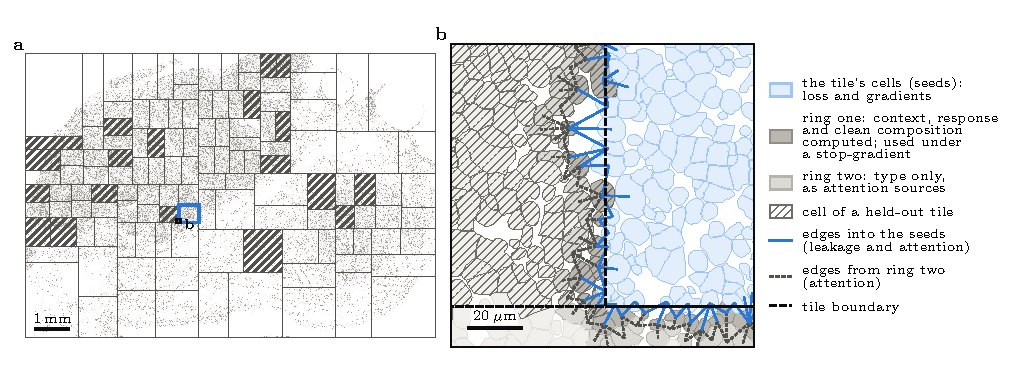
\includegraphics[width=\textwidth]{figures/fig_batching}
\caption{Tiles, the held-out split and the two-hop halo on the primary section. \textbf{a},~The section cut into contiguous tiles of at most $4{,}096$ cells by recursive median split. Hatched tiles are held out ($15\%$ of tiles, one split). The blue tile is shown in b, and the black square marks the window of b. \textbf{b},~Where that training tile meets a held-out tile (left) and another training tile (below). The tile's cells are the seeds, on which the loss is evaluated. Ring one, their graph neighbours, has its context, response and clean composition computed in the same pass. Those compositions enter the seeds' foreign influx under a stop-gradient, and ring one's types are attention sources for the seeds (solid edges). Ring two, the neighbours of ring one, contributes only its types, as attention sources for ring one (dashed edges). Both rings are read from the leakage kernel's own edge list. Hatched cells belong to the held-out tile: ring cells drawn from it enter training as inputs, with no loss and no gradient (\cref{sec:batching}).}
\label{fig:batching}
\end{figure}

\subsection{The Held-Out Probe}
\label{app:probe}

\Cref{fig:probe} shows how the probe of \cref{sec:invariance} is fitted, scored and read.

\begin{figure}[t]
\centering
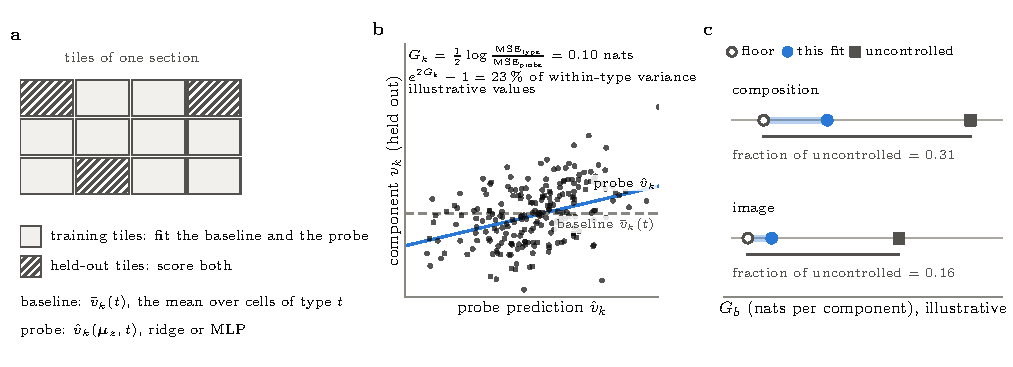
\includegraphics[width=\textwidth]{figures/fig_probe}
\caption{How the held-out probe grades the invariance of $\vz$ (\cref{eq:probe}); schematic, with synthetic values chosen for legibility. \textbf{a},~The type-only baseline and the probe are fitted on the training tiles and scored on the held-out tiles (hatched). The baseline predicts each component of the invariance block by its mean over cells of the same type; the probe predicts it from $(\vmu_z, t)$ with a ridge regression or a small perceptron. \textbf{b},~One component for held-out cells of one type. The baseline's error is the spread around the type mean (dashed), the probe's the spread around its prediction (solid, the line of perfect prediction). $G_k$ is half the log ratio of the two mean squared errors, $e^{2G_k} - 1$ is the share of within-type variance the probe explains, and $G_b$ averages $G_k$ over the block. \textbf{c},~Reading $G_b$ for each block. The floor is its value with $\vmu_z$ permuted within type; the uncontrolled fit is the same model with $\alphaa = 0$. What is reported is this fit's excess over the floor (blue bar) and that excess as a fraction of the uncontrolled fit's (grey bracket), for each probe family. A block passes when that fraction is at most a quarter (dotted guard): here the composition block fails and the image block passes.}
\label{fig:probe}
\end{figure}

\Cref{tab:probe} gives the probe on the final fits of every section.

\begin{table}[t]
\centering
\caption{The held-out probe on the final fits, per section. For each block, the share of its within-type variance that the probe explains from $\vz$ beyond the permutation floor ($e^{2\,\mathrm{excess}} - 1$, in \%), for the model trained without the adversary ($\alphaa = 0$, two seeds) and with it (the final fits, three seeds), the largest share with the adversary that would pass (\emph{needed to pass}: a quarter of the excess without the adversary, as a share), and the quantity the guard reads, the \emph{fraction left}: the excess with the adversary as a fraction of the mean excess without it, $0$ when the adversary removes everything the probe can find and $1$ when it removes nothing. Ranges are over seeds. A seed passes when all four fractions (two blocks, two probes) are at most a quarter. The sections end at a similar absolute residual; the fraction left is larger where less leaked to begin with. Section B of the lung TMA is graded with the models fitted on section A. \pending{regenerate once Unassigned is excluded as a target in the re-read of the final fits}}
\label{tab:probe}
\small
\setlength{\tabcolsep}{5pt}
\begin{tabular}{@{}lccccc@{}}
\toprule
& Ovarian FFPE & Lung FFPE & Ovarian FF & Lung TMA A & Lung TMA B \\
\midrule
\multicolumn{6}{@{}l}{\emph{Composition, MLP probe}} \\
\quad without the adversary (\%) & 19.5--20.8 & 11.8--12.4 & 36.3--37.4 & 5.5--7.0 & 6.8--7.0 \\
\quad with the adversary (\%) & 4.4--5.7 & 3.9--4.7 & 4.4--4.9 & 3.1--4.4 & 3.9--4.6 \\
\quad needed to pass (\%) & 4.7 & 2.9 & 8.2 & 1.5 & 1.7 \\
\quad \textbf{fraction left} & \textbf{0.23--0.30} & \textbf{0.33--0.40} & \textbf{0.14--0.15} & \textbf{0.50--0.71} & \textbf{0.58--0.67} \\
\addlinespace
\multicolumn{6}{@{}l}{\emph{Image, MLP probe}} \\
\quad without the adversary (\%) & 14.8--17.1 & 9.5--10.9 & 34.3--37.0 & 5.8--8.3 & 5.3--7.2 \\
\quad with the adversary (\%) & 2.5--4.1 & 1.4--2.0 & 4.5--4.9 & 2.2--2.8 & 2.0--3.0 \\
\quad needed to pass (\%) & 3.8 & 2.5 & 7.9 & 1.7 & 1.5 \\
\quad \textbf{fraction left} & \textbf{0.17--0.27} & \textbf{0.14--0.20} & \textbf{0.14--0.16} & \textbf{0.32--0.40} & \textbf{0.32--0.49} \\
\addlinespace
\multicolumn{6}{@{}l}{\emph{Ridge probe, fraction left}} \\
\quad composition & 0.16--0.23 & 0.15--0.19 & 0.07--0.08 & 0.19--0.22 & 0.32--0.45 \\
\quad image & 0.08--0.16 & 0.05--0.16 & 0.10--0.13 & 0.19--0.21 & 0.17--0.39 \\
\midrule
Seeds passing & 1/3 & 0/3 & 3/3 & 0/3 & 0/3 \\
\bottomrule
\end{tabular}
\end{table}


\section{EXPERIMENTAL DETAILS}
\label{app:experimental}

\subsection{Sections}
\label{app:sections}

\Cref{tab:sections} lists the sections of \cref{sec:setup}, and \cref{fig:sections} shows them. The lineage classes include Unassigned. On the ovarian FFPE section it also holds a low-depth class of mixed lineage that the curated annotation had named as a tumour subtype, which is why its share is the largest.

\begin{table}[t]
\centering
\caption{The sections. Median counts are per cell over the whole section. The TMA core and its serial section are one core of the microarray on two slides; no model is fitted to the serial section.}
\label{tab:sections}
\small
\setlength{\tabcolsep}{4pt}
\begin{tabular}{@{}llrrrrr@{}}
\toprule
Section & Role & Cells & Genes & Lineage classes & Unassigned (\%) & Median counts \\
\midrule
Ovarian cancer (FFPE) & primary & 407{,}120 & 5{,}101 & 12 & 10.3 & 178 \\
Lung cancer (FFPE) & fitted & 278{,}324 & 5{,}001 & 20 & 0.1 & 242 \\
Ovarian cancer (FF) & fitted & 1{,}157{,}637 & 5{,}001 & 10 & 4.3 & 1{,}401 \\
Lung TMA core & fitted & 69{,}422 & 5{,}001 & 30 & 4.2 & 279 \\
Lung TMA core, serial section & held out & 70{,}757 & 5{,}001 & 30 & 4.8 & 253 \\
\bottomrule
\end{tabular}
\end{table}

\begin{figure}[t]
\centering
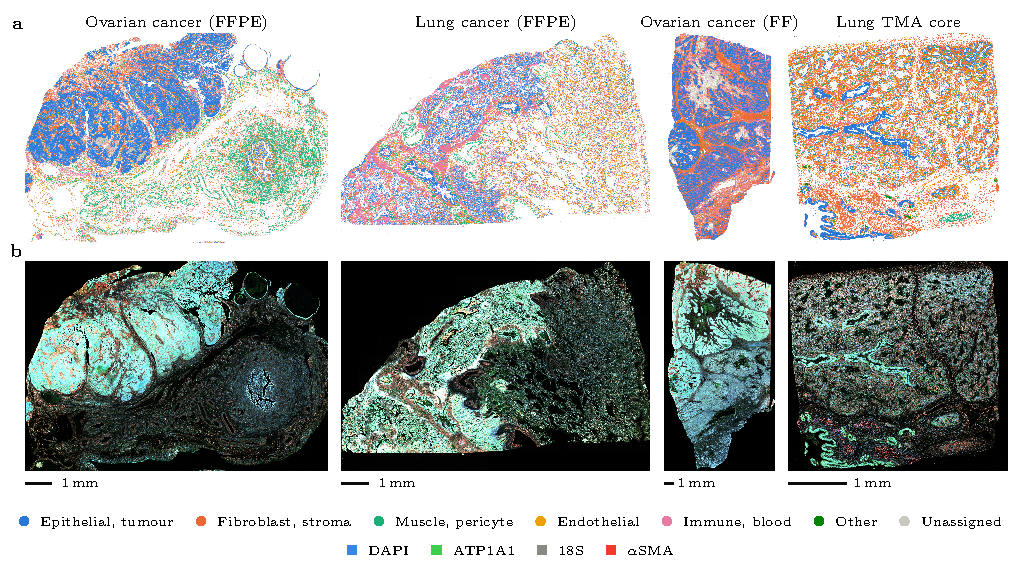
\includegraphics[width=\textwidth]{figures/fig_sections}
\caption{The four fitted sections. \textbf{a},~Every cell at its centroid, coloured by its lineage label, with the labels grouped into six families for display only; the model is fitted with the finer lineage classes of \cref{tab:sections}. \textbf{b},~The morphology image of the same section, the four channels the image descriptor reads, coloured as in \cref{fig:overview}b. The TMA panel is the fitted core only. Each section is shown at its own scale; the bars are $1$\,mm.}
\label{fig:sections}
\end{figure}

\subsection{Lineage Labels}
\label{app:lineage}

The fitted labels are lineage-level on every section (\cref{sec:setting}). States, such as proliferating, activated or hypoxic, and locations, such as tumour- or stroma-associated, are merged into their lineage; lineages and developmentally distinct sub-lineages are kept. The mappings were fixed and recorded before any model was refitted.

\paragraph{Curated annotations.}
On the ovarian FFPE section the eighteen curated classes become twelve (\cref{tab:lineage-ovarian}). Two classes needed a decision. The class named as a SOX2-OT$^+$ tumour subtype is mostly not tumour: its cells have a median of $27$ transcripts against $333$ for tumour cells, three quarters show no SOX2-OT count, and its pooled profile decomposes mostly into macrophage expression, so it is folded into Unassigned rather than into the tumour lineage. The class named as malignant cells lining a cyst expresses mesothelial markers (CALB2, PRG4, BNC1, PDPN, UPK3B) and lacks the tumour markers (EPCAM, PAX8, ESR1), and becomes its own lineage. On the lung TMA the thirty-five curated classes become thirty: the state classes (activated, inflammatory and myofibroblasts, activated endothelium and proliferating cells) are reassigned cell by cell to the sub-lineage their markers indicate, with the cell-cycle genes left out for the proliferating class, and the other classes are kept.

\paragraph{Other judgement calls.}
Four further choices are not forced by the rule and are stated so that they can be revisited. The tumour- and stroma-associated fibroblasts of the ovarian FFPE section are merged, because what separates them is the cancer-associated fibroblast programme, a state, rather than a lineage. Its two endothelial classes are merged too, although what separates them is less clear: a tip-cell state on one side and a weakly venous identity on the other. On the lung TMA the alveolar and adventitial fibroblasts are kept as distinct sub-lineages, and the myofibroblasts, which could belong to either, are split between them by their markers, about evenly. The cell-by-cell reassignment of the TMA's state classes is expected to be right for about three cells in four, and its margins are recorded with the mapping.

\paragraph{Clustered sections.}
On the lung FFPE section and the fresh-frozen ovarian section the labels start from unsupervised clusters, and each cluster is assigned the lineage its marker genes indicate, on the lung TMA's vocabulary for the lung section (\cref{tab:lineage-clusters}). Clusters of immune cells next to tumour that carry some tumour signal keep their immune lineage, since that signal is the leakage the model is built to absorb, and one low-depth cluster of the fresh-frozen section becomes Unassigned.

\begin{table}[t]
\centering
\caption{Lineage labels on the ovarian FFPE section: the curated classes merged into each lineage.}
\label{tab:lineage-ovarian}
\small
\begin{tabular}{@{}>{\raggedright\arraybackslash}p{0.28\textwidth}>{\raggedright\arraybackslash}p{0.62\textwidth}@{}}
\toprule
Lineage & Curated classes \\
\midrule
Ciliated epithelial cells & Ciliated Epithelial Cells \\
Endothelial cells & Stromal Associated Endothelial Cells, Tumor Associated Endothelial Cells \\
Fallopian tube epithelium & Fallopian Tube Epithelium \\
Fibroblasts & Stromal Associated Fibroblasts, Tumor Associated Fibroblasts \\
Macrophages & Macrophages \\
Mesothelial-like cyst lining & Malignant Cells Lining Cyst \\
Pericytes & Pericytes \\
Smooth muscle cells & Smooth Muscle Cells \\
T/NK cells & T and NK Cells \\
Tumour & Inflammatory Tumor Cells, Proliferative Tumor Cells, Tumor Cells, VEGFA+ Tumor Cells \\
Unassigned & SOX2-OT+ Tumor Cells, Unassigned \\
Urothelial-like cells & Urothelial-like Cells \\
\bottomrule
\end{tabular}
\end{table}

\begin{table}[t]
\centering
\caption{Lineage labels on the two clustered sections: the clusters assigned to each lineage.}
\label{tab:lineage-clusters}
\small
\begin{tabular}{@{}>{\raggedright\arraybackslash}p{0.24\textwidth}>{\raggedright\arraybackslash}p{0.13\textwidth}@{\hspace{0.04\textwidth}}>{\raggedright\arraybackslash}p{0.2\textwidth}>{\raggedright\arraybackslash}p{0.33\textwidth}@{}}
\toprule
\multicolumn{2}{@{}l}{Lung cancer (FFPE)} & \multicolumn{2}{l@{}}{Ovarian cancer (FF)} \\
\cmidrule(r){1-2}\cmidrule(l){3-4}
Lineage & Clusters & Lineage & Clusters \\
\midrule
AT1 & 18, 23 & Endothelial cells & 16, 38 \\
AT2 & 20 & Fibroblasts & 7, 13 \\
Adventitial fibroblasts & 4, 17 & Macrophages & 10, 14, 19, 20, 25, 26, 28, 30, 34 \\
Alveolar fibroblasts & 10 & Ovarian stroma & 3, 6, 23 \\
Alveolar macrophages & 16 & Pericytes & 32 \\
B cells & 12 & Plasma cells & 17, 35 \\
EC general capillary & 3, 22, 25 & Smooth muscle cells & 33 \\
EC venous & 13 & T/NK cells & 18, 22, 24, 27, 29, 31, 36, 37 \\
Goblet & 19 & Tumour & 1, 2, 4, 5, 8, 11, 12, 15, 21 \\
Interstitial macrophages & 2 & Unassigned & 9; unclustered cells \\
Mast cells & 27 &  &  \\
Multiciliated & 26, 28 &  &  \\
Neuroendocrine & 31 &  &  \\
Neutrophils & 6 &  &  \\
Pericytes & 24 &  &  \\
Plasma cells & 15 &  &  \\
Smooth muscle & 5 &  &  \\
T/NK cells & 1, 7, 21, 30, 32 &  &  \\
Tumour & 8, 9, 11, 14, 29 &  &  \\
Unassigned & unclustered cells &  &  \\
\bottomrule
\end{tabular}
\end{table}

\subsection{Baselines}
\label{app:baselines}

\Cref{tab:baselines} gives the configuration of each comparison method. Every method is run at its published defaults, and on our pruned Delaunay graph where it accepts an external graph; resolVI and MintFlow build their own. The methods that read a label read the lineage labels. SIMVI does not read one, so refitting it at lineage labels only checks reproducibility.

\begin{table}[t]
\centering
\caption{Comparison methods as run. Versions are the package versions used.}
\label{tab:baselines}
\small
\setlength{\tabcolsep}{4pt}
\begin{tabular}{@{}>{\raggedright\arraybackslash}p{0.11\textwidth}>{\raggedright\arraybackslash}p{0.2\textwidth}>{\raggedright\arraybackslash}p{0.22\textwidth}>{\raggedright\arraybackslash}p{0.13\textwidth}>{\raggedright\arraybackslash}p{0.24\textwidth}@{}}
\toprule
Method & Version & Graph & Label & Budget and coverage \\
\midrule
resolVI & scvi-tools 1.5.1 & own, 10 nearest neighbours & lineage & 50 epochs; every section \\
SIMVI & simvi 0.1.2 (scvi-tools 0.16.1) & ours & not used & package default; the TMA core and its serial section; failed on the fresh-frozen section (the whole section does not fit in GPU memory); not attempted on the two FFPE sections \\
MintFlow & mintflow 0.3.0 & own Delaunay graph & lineage & width 600, 50 epochs; the TMA core, transferred to its serial section; failed on the fresh-frozen section (out of host memory before training); not attempted on the two FFPE sections \\
Cellina & cellina 1.1.1 (scvi-tools 1.2.0) & ours & lineage & package default; being run \\
\bottomrule
\end{tabular}
\end{table}

\subsection{Assets and Licences}
\label{app:assets}

The ovarian FFPE, lung FFPE and fresh-frozen ovarian sections are public datasets of 10x Genomics \citep{tenx_ovarian_ffpe,tenx_lung_ffpe,tenx_ovary_ff}, released under the Creative Commons Attribution 4.0 International licence (CC BY 4.0). The TMA core and its serial section are two samples of GEO series GSE315411 \citep{williamskatek2026fishing}; NCBI places no restriction on the use or distribution of GEO data, while noting that submitters may claim rights in the data they submit \todo{verify the wording on the GEO disclaimer page}. The image model KRONOS and its successor KRONOS2 \citep{kronos2025} are released under CC BY-NC-ND~4.0, for non-commercial academic research and after registration; we use them for that purpose and redistribute neither. The comparison methods are released under the BSD 3-Clause licence: scvi-tools, which contains resolVI, SIMVI, MintFlow and Cellina. The code will be released on acceptance; no new data are released.

\subsection{Training Cost}
\label{app:timing}

\Cref{tab:timing} gives the cost of a fit. DISCELL's time per epoch is pure training, measured over twenty epochs with no evaluation. Its wall-clock time covers the three final fits, including evaluations every five epochs and the early stop. The comparison methods' times are whole fits, as recorded when they were run.

In symbols, a training step on a tile of $n$ seeds with $n_1$ cells in ring one costs $O((n + n_1)\,G h)$ in the encoders and decoder, for hidden width $h$, and $O(|E_n|\,G)$ in the foreign influx, for the $|E_n|$ edges into the seeds (\cref{sec:batching}). The six adversary head updates add $O\big(6\,(n + n_1)\,h_a(\dz + K)\big)$ with $h_a = 64$, small beside the gene-sized terms because $\dz$ and $K$ are far below $G$. An epoch visits every training tile once, so its cost is linear in the number of cells; the held-out probes are fitted on at most $30{,}000$ cells whatever the section's size. Peak memory is the section's count matrix, held resident, plus the gathered edge-by-gene rows of the influx, $O(|E_n|\,G)$ per step, which the tile size bounds. The leakage sweep multiplies the cost of a fit by its six grid points and three seeds, eighteen fits per section. Sample size is not analysed: how many cells a section needs for the readouts to stabilise is not studied beyond the range of sizes in \cref{tab:sections}.

\begin{table}[t]
\centering
\caption{Model size and training cost on one GPU. \emph{Peak memory}: largest allocation during training, with the section resident on the GPU. \emph{Run time}: one whole fit, for DISCELL including its evaluations every five epochs and the early stop, as the range over the three seeds of the final configuration. Where a method has no time, the reason is given: \emph{not attempted} means it was never run on that section, \emph{failed} that it was run and did not complete.}
\label{tab:timing}
\small
\setlength{\tabcolsep}{4pt}
\begin{tabular}{@{}lrrrr@{}}
\toprule
& Ovarian (FFPE) & Lung (FFPE) & Ovarian (FF) & Lung TMA core \\
\midrule
\multicolumn{5}{@{}l}{\emph{DISCELL, model and training details}} \\
\quad parameters (M) & 4.19 & 4.12 & 4.11 & 4.13 \\
\quad peak memory (GiB) & 6.3 & 4.3 & 15.1 & 1.4 \\
\quad epochs to the stop & 105--115 & 80--100 & 175--230 & 85--90 \\
\quad s per epoch, training only & 1.98 & 1.35 & 5.78 & 0.45 \\
\addlinespace
\multicolumn{5}{@{}l}{\emph{Run time of one fit (min)}} \\
\quad DISCELL & 8.7--9.3 & 3.2--7.4 & 31.2--43.4 & 1.3 \\
\quad resolVI & 32.8 & 22.0 & 105.0 & 5.5 \\
\quad SIMVI & not attempted$^{a}$ & not attempted$^{a}$ & failed$^{b}$ & 107.2 \\
\quad MintFlow, 50 epochs & not attempted$^{c}$ & not attempted$^{c}$ & failed$^{d}$ & 680.1 \\
\bottomrule
\end{tabular}
\par\smallskip
\parbox{0.9\textwidth}{\footnotesize $^{a}$ Run only on the TMA core, where it fits whole; not attempted on the two FFPE sections. $^{b}$ SIMVI passes the whole graph through the network at every step, and the whole fresh-frozen section does not fit in GPU memory. We report only methods run on whole sections, so an earlier run on a window of the section is not used. $^{c}$ Run only on the TMA core, where one fit took about eleven hours for $70{,}000$ cells; not attempted on the larger FFPE sections. $^{d}$ Ran out of host memory while building its inputs, before training started.}
\end{table}

\subsection{Planted Worlds}
\label{app:planted}

Three questions about the fitting procedure are answered on simulated sections, where the truth is known.

\paragraph{The amortisation gap: what is measured.}
The intrinsic encoder $q(\vz_i \mid \vx_i, t_i)$ reads a cell's counts and type but not the foreign influx $\rhobar_i$, although the counts contain it. Its posterior mean can therefore differ from the exact posterior mean $\E[\vz_i \mid \vx_i, t_i, \rhobar_i]$ that a model told the influx would reach. This difference, the amortisation gap, cannot be measured on tissue, where the exact posterior is unknown, so we measure it on simulated sections for which the exact posterior can be computed.

\paragraph{The simulation.}
Each simulated section follows DISCELL's generative model with the response switched off, so that every quantity lies inside the model class the fit assumes and a gap measured here is a gap of inference, not of model mismatch.
\begin{itemize}
\item \emph{Cells and types.} $3{,}000$ cells at uniformly random positions in a $700\um$ square, and four types laid out in spatial patches: each cell takes the type of the nearest of twelve anchor points, three per type, up to a random perturbation, so that neighbours are often of another type and leakage mixes types, as in tissue.
\item \emph{Intrinsic state and composition.} $\vz_i \sim \N(\mathbf{m}_{t_i}, 0.5^2\vI)$ in two dimensions, with type means $\mathbf{m}_t \sim \N(\mathbf{0}, 1.5^2\vI)$, and a clean composition $\vrho_i = \softmax(\vz_i\mathbf{A})$ over forty genes, with loadings $\mathbf{A}$ drawn from a standard normal.
\item \emph{Leakage.} The Delaunay graph of the positions, pruned at $40\um$, with the kernel $\beta_{ij} \propto \exp(-d_{ij}/\tau)$, $\tau = 20\um$, normalised over each cell's neighbours: the model's own kernel with every face set to one. The leak fraction is $\kappa = 0.2$, and $\rhobar_i = \sum_j \beta_{ij}\vrho_j$.
\item \emph{Counts.} A depth $\ell_i \sim \Pois(D)$, at least $20$, for $D \in \{100, 300, 1{,}000\}$, and $\vx_i \sim \Mult\big(\ell_i, (1-\kappa)\vrho_i + \kappa\rhobar_i\big)$.
\item \emph{Image descriptor.} An eight-dimensional vector made from the cell's neighbour composition plus noise, so that the context has something to read.
\end{itemize}

\paragraph{The exact posterior.}
Given $\rhobar_i$, $\kappa$, $\mathbf{A}$, $\mathbf{m}_{t_i}$ and $\ell_i$, the posterior of $\vz_i$ is a two-dimensional density. It has no closed form, since the multinomial and the softmax are not conjugate, but in two dimensions its mean and covariance are computed to numerical precision on a $129 \times 129$ grid centred on its mode.

\paragraph{The fit and the comparison.}
DISCELL is fitted to the counts with a two-dimensional $\vz$ and its response channel present, as on tissue, for $300$ epochs, at the true leak fraction and at leak fractions off by up to $0.1$ either way. Because $\vz$ is identified only up to a smooth invertible map, the encoder's posterior means are first mapped onto the simulation's coordinates by a small network with five-fold cross-fitting; since the means are two-dimensional, the map cannot add information the encoder did not keep. The gap of a cell is the distance between its mapped mean and the exact mean, divided by the size of the exact posterior's standard deviation, and it is averaged over cells and over three seeds. Four references are fitted to the exact posterior mean directly, also with cross-fitting: a multilayer perceptron given the encoder's inputs, the same perceptron given $\rhobar_i$ as well, which the encoder never sees, a linear regression on the encoder's inputs, and the type mean, which knows no counts.

\paragraph{The result.}
At the true leak fraction the encoder's gap is below that of the perceptron trained directly on the same inputs, at every depth, and close to that of the perceptron that also sees $\rhobar_i$ (\cref{tab:planted-gap}): not seeing the influx costs little. The gap grows with depth only in units of the posterior width, because the posterior narrows as the depth increases; in units of $\vz$ itself it is flat. A wrong leak fraction enlarges it by at most a tenth over the mismatches tried, and it is smallest at the true value. The references are regression models of finite capacity, not information bounds, so these statements are comparative.

\begin{table}[t]
\centering
\caption{Amortisation gap on the simulated sections at the true leak fraction: the distance between an estimate of the posterior mean of $\vz$ and the exact one, in units of the exact posterior standard deviation, averaged over cells, mean of three seeds, by sequencing depth $D$. The DISCELL encoder is trained without the exact posterior; the other rows are fitted to it directly.}
\label{tab:planted-gap}
\small
\begin{tabular}{@{}lrrr@{}}
\toprule
& \multicolumn{3}{c}{Depth $D$} \\
\cmidrule(l){2-4}
Estimate of the posterior mean & 100 & 300 & 1{,}000 \\
\midrule
DISCELL encoder & 0.55 & 0.83 & 1.48 \\
Perceptron, the encoder's inputs & 0.61 & 0.95 & 1.61 \\
Perceptron, the encoder's inputs and $\rhobar_i$ & 0.53 & 0.80 & 1.35 \\
Linear regression, the encoder's inputs & 1.40 & 2.50 & 4.53 \\
Type mean & 2.4 & 4.1 & 7.4 \\
\bottomrule
\end{tabular}
\end{table}

\paragraph{A leak-subtracted encoder input.}
The intrinsic encoder could be given counts from which the expected foreign influx has been subtracted, rather than the raw counts. On planted worlds with a known leak, this helped on one of three worlds. In a follow-up with twelve seeds it reversed on three of the six seeds where the comparison was not saturated, and it cost up to twenty-two points of recall of the planted signal. The encoder therefore reads raw counts, and the subtraction is kept as an option, off by default.

\paragraph{A dead response channel.}
A fit can end with a response that carries no information about the niche: the divergence of $\vw$ to its prior collapses and the context is ignored. Two checks flag it. During training, a summed divergence of $\vw$ below $10^{-5}$ over the first twenty epochs marks the fit. After training, the information between $\vw$ and the niche, on held-out cells and against a within-type permutation floor, must exceed its floor. Among the archived fits of the development period, twelve had a dead channel, nine of them on the deepest section. The KL warm-up of the final configuration removed it in every one of eight refits of that section, and the checks flag no final fit.

\section{LIMITATIONS}
\label{app:limitations}
\readorder{3}

The conclusion names the main limitations. Each is argued where it arises in the paper; this appendix collects them all, with what each one implies.
\begin{itemize}
\item \emph{The form of the leakage.} The leak fraction is one number per section, the leakage is the same for every gene and scales with the receiving cell's depth, and there is no ambient term (\cref{sec:generative}). A per-cell or per-gene variation in contamination is not covered by the sweep; its sensitivity to the leak's form is checked on the primary section only, where three other forms move no read by more than $1.3$ seed standard deviations, but a fixed false-positive floor lowers the transport read from $0.65$ to $0.50$, a move of $8.3$ standard deviations (\cref{app:sensitivity}).
\item \emph{What the sweep separates.} It separates a spatial association from leakage of the modelled form, not from spatially organised intrinsic variation within a type, which the conditional invariance assigns to the response, nor from cells selecting their niche (\cref{sec:sweep}).
\item \emph{Labels.} The labels come from the same contaminated counts, and the decomposition is relative to their granularity: a state merged into its lineage becomes variation the model must place, and a spatially clustered state merged in this way is read as a response (\cref{sec:setting,sec:invariance}).
\item \emph{The invariance is incomplete.} With the adversary, a nonlinear probe still recovers $3.5$ to $5.5\%$ of the within-type variance of neighbour composition from the intrinsic state on every section; where little leaked to begin with, as on the TMA core, the adversary removes only $29$ to $48\%$ of what the uncontrolled model leaves. A probe at its floor bounds only the dependence it can detect (\cref{tab:probe}).
\item \emph{The response at the operating point.} With the response weight far above its bound-equivalent value, the response readouts are in effect readouts of the context regression, except that on the lung section the response separates some merged clusters better than its prior mean (\cref{app:subtype}); the per-cell channel is closed by design, not by the data: a per-cell response planted in simulation is not detected at this weight and is partly absorbed by the intrinsic state (\cref{sec:objective}, \cref{app:planted-percell}). Several response readouts are also not specific to it: ligand--receptor genes take a larger share of the leakage channel than other genes on every section, so that criterion is met by leakage alone; the lean of the programmes toward membrane and secreted genes is what a gene-specific leak would produce, and the band ordering on the primary section is also followed by the intrinsic state and by depth (\cref{app:response}).
\item \emph{The cycle reference.} The cell-cycle scores against which the intrinsic state is graded are gene-set scores of the cell's own segmented counts, not an independent measurement: transcripts leaked from cycling neighbours and expression induced by the environment enter them, so the asymmetry between the latents shows where the model places this axis of the counts, not that it is the cell's own (\cref{sec:results-z}).
\item \emph{Inference.} The intrinsic encoder does not see the foreign influx, so its posterior mean can differ from the exact one; in simulation, at the final configuration, the difference is measurable, $0.65$ to $1.93$ posterior standard deviations, and larger at every depth than that of a perceptron fitted to the exact posterior mean from the same inputs, and on tissue it cannot be measured (\cref{app:planted}). The posterior family is a compromise, so the uncertainty reported comes from the sweep and the seeds, not from the posterior (\cref{sec:inference}).
\item \emph{Identification.} Beyond the upper bound on the leak fraction and the invariance the probe grades, nothing guarantees that the intrinsic and response coordinates are identified (\cref{sec:sweep}).
\item \emph{Evaluation.} Cells of held-out tiles enter training as neighbours under a stop-gradient (\cref{sec:batching}), every fit is to one section, and only one section is held out whole. Most cells scored by the transport reads lie in the model's training tiles; scored on held-out tiles only, the fraction of the ceiling moves in both directions and Read A falls (\cref{tab:transport-heldout}). The comparison methods were fitted on our held-out cells too, as their software is designed, and at their published defaults, while DISCELL's weights were calibrated on these sections (\cref{sec:setup}); two of them could not be run on some of the sections on the resources currently available (\cref{tab:baselines}).
\end{itemize}

\section{SYNTHETIC RECOVERY}
\label{app:synthetic}
\readorder{16}

\paragraph{Goal.} Check, on data simulated from the model's own generative story, that the final configuration recovers the planted intrinsic states, responses and gene programmes, that the adversary keeps the planted niche out of $\vz$, and how much a wrong leak fraction costs. A second simulation (\cref{app:planted-percell}) asks whether the response channel detects a per-cell response that the niche does not predict.

\paragraph{Generative process.} $N = 6{,}000$ cells uniformly in a $1{,}000\um$ box; $K = 8$ types assigned by a soft Voronoi partition around random anchors with Gumbel noise so that types cluster in space; the graph, kernel, composition and rings built by the same procedure as for real data from a Delaunay triangulation, with unit face lengths so that $\beta \propto \exp(-d/\tau)$ only; $\vz_i \sim \N(\mathbf{m}_{t_i}, 0.5^2\vI)$ with type means $\mathbf{m}_t \sim \N(\mathbf{0}, 1.5^2\vI)$; a planted response $\vw_i = \mathbf{M}^\top\vy_i + 0.3\,\boldsymbol\varepsilon_i$ linear in the true neighbour composition; $\log\vrho_i = \mathbf{A}\vz_i + \vB\vw_i$ (up to normalisation) with standard-normal loadings; $\rhobar_i$ the kernel-weighted neighbour average; $\vp_i$ the renormalised mixture at the planted $\kappa$; totals $\ell_i \sim \max(\Pois(150), 20)$; $\vx_i \sim \Mult(\ell_i, \vp_i)$; and a planted image descriptor $\vPhi_i = \mathbf{P}^\top\vy_i + 0.4\,\boldsymbol\varepsilon'_i$ in eight dimensions. $G = 60$ genes, planted $\dz = 4$, $\dw = 2$. Three worlds, drawn from three simulator seeds, at each planted $\kappa \in \{0, 0.2\}$.

\paragraph{Fit.} The final configuration (\cref{tab:architecture}), with the widths reduced to the small world ($\dz = 8$, $\dw = 2$, hidden width $128$, attention width $16$) and tiles of $512$ cells: the adversary at $\alphaa = 0.3$ with its composition term weighted three times, $\alphaw = 0.1$ with its warm-up over thirty epochs, $\alphaz = \tfrac12/\lbar$ with $\lbar$ the simulated section's median count ($150$, so $\alphaz \approx 0.0033$), $\omega = 1$, and the budget of $500$ epochs with patience $40$, with $15\%$ of the tiles held out for the stopping rule of \cref{sec:selection}. Every readout is taken on all cells at the accepted checkpoint. The uncontrolled arm is the same fit at $\alphaa = 0$. Each world is fitted with three model seeds, so every arm has nine fits. In the misspecified arms, the worlds planted at $\kappa = 0.2$ are fitted at each assumed $\kappa \in \{0, 0.1, 0.2, 0.3, 0.4\}$.

\paragraph{Readouts.} The agreement with the planted type, as the normalised mutual information between the planted types and a $k$-means clustering of $\vmu_z$ with $k = K$, against two references: the same clustering of the leading principal components of the log-normalised counts, which is what the counts alone support, and of the planted $\vz$ itself; the first canonical correlation between $\vmu_w$ and the planted response; the largest principal-angle cosine between the column spaces of the fitted and the planted loadings, against random two-dimensional subspaces of $\R^{60}$, whose cosine has a mean of $0.23$ and a $95$th percentile of $0.37$ to $0.38$ over $2{,}000$ draws; and the within-type coefficient of determination of the centred neighbour composition on $\vmu_z$, which is zero for the planted $\vz$.

\paragraph{Result.} \flag{TRIM}{long; the development-run bistability sentence is history, one clause suffices} At the matched leak fraction the final configuration recovers each planted quantity on every world (\cref{tab:synthetic}). The agreement of $\vmu_z$ with the planted type is $0.80$ to $0.96$, about what the counts support or more ($0.69$ to $0.93$; above the world's count clusters in seventeen fits of eighteen, and below them in one, $0.80$ against $0.83$) and short of the planted $\vz$ ($0.91$ to $0.98$), which is not reachable at $150$ counts per cell. The response correlates with the planted one at $0.83$ to $0.95$. The loadings are recovered above the random reference in every fit, at a cosine of $0.63$ to $0.99$; their recovery varies between seeds on some worlds, at both planted leak fractions (one fit of one world at $\kappa = 0$ reaches only $0.63$), which is why no gene-level statement on tissue is made from one fit (\cref{sec:sweep}). The intrinsic state carries almost none of the planted niche: the within-type $R^2$ of composition on $\vmu_z$ is at most $0.04$, against $0.11$ to $0.19$ without the adversary. Without the adversary the response and the loadings are also recovered worse and less reliably (canonical correlation $0.29$ to $0.91$, loadings $0.14$ to $0.85$). An earlier development run, at a configuration that is no longer used, had suggested that the loadings are bistable between seeds under a planted leak and stable without one; at the final configuration the spread between seeds is wider without a planted leak than under one: per world, the cosines span $0.63$ to $0.99$, $0.97$ to $0.99$ and $0.70$ to $0.98$ at $\kappa = 0$, against $0.98$ to $0.99$, $0.99$ and $0.77$ to $0.99$ at the matched $\kappa = 0.2$. Fitted at a wrong leak fraction, anywhere from $0$ to $0.4$ on worlds planted at $0.2$, the recovery moves little (\cref{fig:synthetic-misspec}): agreement $0.79$ to $0.97$, canonical correlation $0.78$ to $0.94$ (the lowest at an assumed $\kappa = 0$), loadings $0.71$ to $1.00$, composition $R^2$ at most $0.01$. On these worlds a leak fraction wrong by up to $0.2$ in either direction costs little of what is recovered. This also means that recovery does not point to the planted leak fraction, and it says nothing about leakage of a form the model cannot represent.

\paragraph{Simulator checks.} Leakage raises the kernel-weighted cosine between a cell's composition and its neighbours' by $0.22$ to $0.26$ at $\kappa = 0.4$ relative to $\kappa = 0$; the planted response is linearly predictable from composition ($R^2$ of $0.75$ to $0.87$); and the mixture is exactly the renormalised convex combination. These worlds have no isolated cells, so the reduction of the mixture to $\vrho$ for an isolated cell is not exercised here.

% Generated table: tab:synthetic. DO NOT EDIT BY HAND; regenerate instead.
% Command: python scripts/paper_tables.py
% Generated: 2026-10-01 17:35:54 (results frozen 2026-09-29 15:07:21, last line of scripts/logs/unassigned_2026-09-28/queue.log)
%
% Sources read (modification time):
%   data/datasets/synthetic_smoke/experiments/synthetic_recovery.json  (2026-09-29 16:58:56)  [after the freeze; see checks]
%
% Reading convention:
%   [min, max] over 3 world seeds x 3 model seeds per arm; best checkpoint; all 6,000 cells
%
% Provenance (row / column -> file : key):
%   every row: data/datasets/synthetic_smoke/experiments/synthetic_recovery.json : groups[arm, planted_kappa, assumed_kappa].fits[*] (min, max over world x model seeds; checked against the group's stored summary); references: world_references[planted kappa].<key> min, max over both planted kappa
%
% Checks and notes:
%   - Final arm configuration (config_final_arm): adv_comp_weight 3.0, alpha_w 0.1,
%     w_warmup_epochs 30, alpha_z 0.003333, epochs 500/patience 40, d_z 8, d_w 2, tile_cells
%     512, val_fraction 0.15. Simulator checks: all pass.
%   - Written 2026-09-29 16:58 (after the freeze; a new run,
%     scripts/logs/synthetic_2026-09-29/AGENT_REPORT.md).
%
% Pending cells:
%   none
%
\begin{table}[t]
\centering
\caption{Recovery on simulated sections, scaled to the simulated world: three worlds per planted \termSpillFrac{}, each fitted with three model seeds; the range over the 9 fits of each row. NMI of $\vmu_z$ with the planted type; \emph{CCA}: first canonical correlation of $\vmu_w$ with the planted response; \emph{Loadings}: principal-angle cosine of the fitted against the planted loadings; \emph{Comp.\ $R^2$}: within-type $R^2$ of neighbour composition from $\vmu_z$. Bold: the matched $\kappa$. \emph{References}: NMI of clusters of the counts and of the planted intrinsic state, composition $R^2$ of the planted state, and the loading cosine of a random subspace (mean and 95th percentile), each the range over the three worlds and both planted rates. A fit is stopped early on $15\%$ of held-out tiles; every read covers all cells. Arrows give the preferred direction.}
\label{tab:synthetic}
\small
\setlength{\tabcolsep}{3pt}
\begin{tabular}{@{}lcccc@{}}
\toprule
Arm & NMI, $\vmu_z$ $\uparrow$ & CCA, $\vw$ $\uparrow$ & Loadings $\uparrow$ & Comp.\ $R^2$ $\downarrow$ \\
\midrule
\multicolumn{5}{@{}l}{\emph{Assumed $\kappa$ = planted $\kappa$}} \\
\quad final configuration, $\kappa = 0$ & 0.80--0.96 & 0.85--0.95 & 0.63--0.99 & 0.00--0.04 \\
\quad without the adversary, $\kappa = 0$ & 0.71--0.94 & 0.29--0.91 & 0.14--0.78 & 0.11--0.19 \\
\quad final configuration, $\kappa = 0.2$ & 0.81--0.96 & 0.83--0.94 & 0.77--0.99 & 0.00--0.02 \\
\quad without the adversary, $\kappa = 0.2$ & 0.71--0.93 & 0.38--0.90 & 0.18--0.85 & 0.12--0.19 \\
\addlinespace
\multicolumn{5}{@{}l}{\emph{Planted $\kappa = 0.2$, final configuration, assumed $\kappa$:}} \\
\quad 0 & 0.86--0.96 & 0.78--0.94 & 0.75--0.96 & 0.00--0.01 \\
\quad 0.1 & 0.82--0.96 & 0.84--0.94 & 0.78--0.99 & 0.00--0.01 \\
\quad \textbf{0.2} & 0.81--0.96 & 0.83--0.94 & 0.77--0.99 & 0.00--0.02 \\
\quad 0.3 & 0.80--0.97 & 0.83--0.94 & 0.74--1.00 & 0.00--0.01 \\
\quad 0.4 & 0.79--0.97 & 0.83--0.94 & 0.71--1.00 & 0.00--0.01 \\
\addlinespace
\multicolumn{5}{@{}l}{\emph{References of the simulated worlds}} \\
\quad clusters of the counts & 0.69--0.93 & -- & -- & -- \\
\quad planted $\vz$ & 0.91--0.98 & -- & -- & 0.00 \\
\quad random subspace, mean & -- & -- & 0.23 & -- \\
\quad random subspace, 95th percentile & -- & -- & 0.37--0.38 & -- \\
\bottomrule
\end{tabular}
\end{table}


\begin{figure*}[t]
\centering
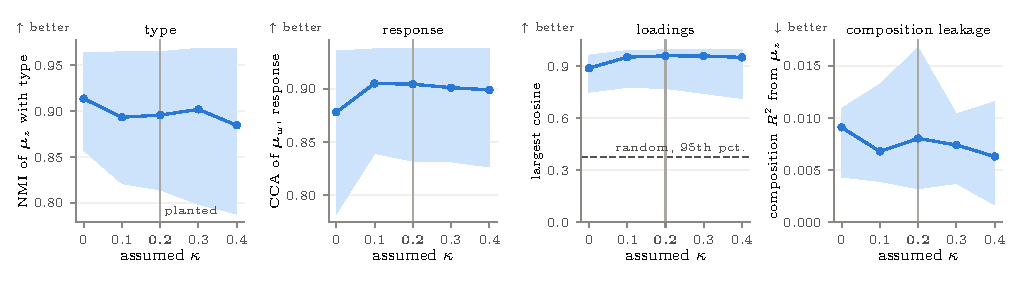
\includegraphics[width=\textwidth]{figures/fig_synthetic_misspec}
\caption{Recovery on the worlds simulated at $\kappa = 0.2$, fitted at each assumed $\kappa$: NMI of $\vmu_z$ with the planted type; the first canonical correlation of $\vmu_w$ with the planted response; the largest principal-angle cosine of the fitted against the planted loadings (dashed: the $95$th percentile of random subspaces); the within-type $R^2$ of neighbour composition on $\vmu_z$. Line: mean over nine fits, three worlds with three model seeds each; band: their range, which is mostly the spread between worlds. The vertical line marks the planted value. Arrows point toward the better direction. The values are in \cref{tab:synthetic}.}
\label{fig:synthetic-misspec}
\end{figure*}

\subsection{A Planted Per-Cell Response}
\label{app:planted-percell}

\flag{KEEP-CORE}{closes thread point 4: channel closed by design, not by the data} At the operating point the response posterior adds almost nothing on the four sections: about one part in a thousand of held-out reconstruction (\cref{tab:recon-modes}), and a per-cell divergence whose ranking of cells does not reproduce between seeds (\cref{app:kl-maps}). Either these tissues carry little per-cell response beyond what the niche predicts, or the weight $\alphaw = 0.1$ closes the channel whatever the data (\cref{sec:objective}). On tissue the two cannot be told apart, so we plant a per-cell response and ask whether the channel finds it.

\paragraph{The plant.} On the worlds planted at $\kappa = 0.2$ above, in $10\%$ of the cells of the most abundant type, drawn at random and therefore spread across niches, the log-rate is shifted along the first axis of the planted response programme, with norm $s$ times the size of the planted niche effect (the root mean square over cells of the planted niche shift of the log-rate), for $s \in \{0, 0.5, 1, 2\}$; $s = 0$ is the recovery world itself. The subset cannot be predicted from neighbour composition, nor from composition and the image descriptor: a five-fold cross-validated classifier within the planted type reaches an AUC of $0.44$ to $0.54$ on all three worlds. The shift lies inside the planted response programme deliberately. A per-cell shift unrelated to the niche is something the intrinsic state may legitimately carry, since the invariance only keeps the niche out of $\vz$; a shift along the response programme is a cell responding more or less strongly than its niche predicts, which is what the per-cell channel exists to carry. The fit is the final configuration unchanged, with three model seeds on world 0, and, as a replication outside the rule, on worlds 1 and 2.

\paragraph{The rule, fixed in advance.} The channel detects a response of strength $s$ if, on world 0, every seed separates the planted cells from the other cells of their type by their response divergence $\KL(q(\vw_i)\,\|\,p(\vw_i \mid \vc_i, t_i))$ with an AUC of at least $0.8$, and every pair of seeds ranks the cells' divergences with a Spearman correlation of at least $0.5$. The smallest $s$ detected was to be reported; if none were detected, that finding would be reported instead: at this weight the channel is closed by design, not by the data.

\paragraph{Result.} \flag{TRIM}{last four sentences repeat 3.5 and app:kl-maps} No strength is detected, on world 0 or on either replication (\cref{fig:planted-percell}, \cref{tab:planted-percell}). The divergence separates the planted cells only partly and not on every seed (AUC $0.66$ to $0.85$ at $s = 1$ and $0.56$ to $0.69$ at $s = 2$ on world 0), and a plant does not make the seeds agree more on the per-cell divergences: on world 0 they agree less at $s = 0.5$ and $s = 1$ than without a plant (Spearman $0.34$ to $0.36$ and $0.11$ to $0.18$, against $0.39$ to $0.41$ at $s = 0$) and about as much at $s = 2$ ($0.25$ to $0.42$); on world 1 they agree less at every strength, and on world 2 about as much as without a plant. The rule's agreement criterion is read over the whole map, and even the null does not reach it. The response's own deviation from its prior mean moves toward the plant, but weakly (correlation $0.11$ to $0.41$ for $s > 0$ over the three worlds), and the held-out gain from it on the planted cells stays below $0.02$ nats per count. As the plant grows, it is increasingly absorbed by the intrinsic state instead: read through the decoder along the planted direction, the correlation of $\vmu_z$ with the plant rises from at most $0.05$ at $s = 0$ to $0.36$ to $0.48$ on world 0, $0.86$ to $0.88$ on world 1 and $0.52$ to $0.70$ on world 2 at $s = 2$. At this weight the per-cell channel is therefore closed by design, not by the data: a per-cell response twice the size of the niche effect, planted where the model is meant to put it, is not found in the response's divergence, and much of it goes to $\vz$. On the four sections the response adds almost nothing to reconstruction beyond the context regression $\mpsi(\vc_i, t_i)$, and on three of them it also reads the merged sublabels as its prior mean does (on the lung section it separates some clusters better, \cref{app:subtype}); the absence of reproducible per-cell structure in its divergence there (\cref{app:kl-maps}) says nothing about whether the tissue has any. What opening the channel costs on tissue is in \cref{app:sensitivity}.

\begin{figure*}[t]
\centering
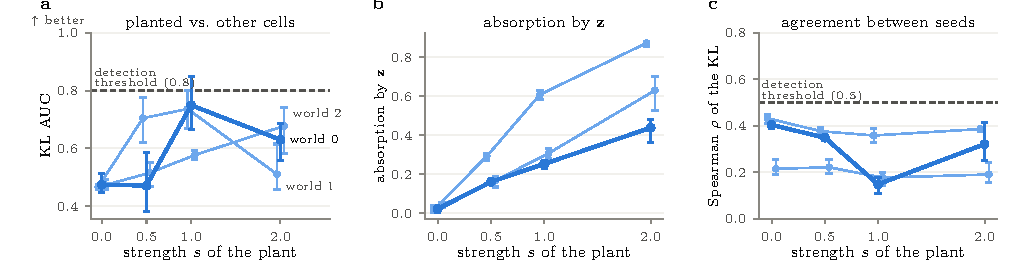
\includegraphics[width=\textwidth]{figures/fig_planted_percell}
\caption{The planted per-cell response against its strength $s$. \textbf{a},~KL AUC separating the planted cells from the other cells of their type by their response divergence; \textbf{b},~absorption of the plant by the intrinsic latent, read through the decoder along the planted direction; \textbf{c},~the Spearman correlation of the per-cell divergence between seeds. World 0, on which the rule fixed in advance decides, in bold; worlds 1 and 2, replications, lighter. Points: mean over three model seeds (seed pairs in c); bars: their range. Dashed: the rule's detection thresholds, a KL AUC of at least $0.8$ in every seed and a Spearman correlation of at least $0.5$ in every seed pair. Arrows point toward the better direction; absorption and the agreement between seeds have none. The values are in \cref{tab:planted-percell}.}
\label{fig:planted-percell}
\end{figure*}

% Generated table: tab:planted-percell. DO NOT EDIT BY HAND; regenerate instead.
% Command: python scripts/paper_tables.py
% Generated: 2026-09-30 11:59:21 (results frozen 2026-09-29 15:07:21, last line of scripts/logs/unassigned_2026-09-28/queue.log)
%
% Sources read (modification time):
%   data/datasets/synthetic_smoke/experiments/planted_percell.json  (2026-09-29 17:49:51)  [after the freeze; see checks]
%
% Reading convention:
%   [min, max] over model seeds 0-2 (seed pairs for Spearman and top-decile overlap) per world
%   and s
%
% Provenance (row / column -> file : key):
%   every row: data/datasets/synthetic_smoke/experiments/planted_percell.json : groups[world, s] per_seed[*] (KL AUC, w corr, z absorption, recon_gain_planted.gain_per_count) and cross_seed[*] (Spearman, top-decile overlap), min-max, checked against the group summary; detected from the group, checked against rule.by_s; predictability[world].*_auc
%
% Checks and notes:
%   - Written 2026-09-29 17:49 (after the freeze; a new run,
%     scripts/logs/planted_percell_2026-09-29/AGENT_REPORT.md). Smallest detected s on world 0:
%     None.
%
% Pending cells:
%   none
%
\begin{table}[t]
\centering
\caption{A planted per-cell response on simulated sections (planted $\kappa = 0.2$, final configuration unchanged). In $10\%$ of the cells of one type, spread across niches, the log-rate is shifted along the planted response programme by $s$ times the size of the planted niche effect (\emph{Shift}, its norm in log-rate units); $s = 0$ is the null. \emph{KL AUC}: the per-cell divergence of the response posterior from its prior separating the planted cells from the other cells of their type; \emph{$\vw$ corr.}: correlation of the response's deviation from its prior mean, along the planted direction, with the plant; \emph{$\vz$ absorption}: the same for the intrinsic latent, read through the decoder along the planted direction; \emph{Recon. gain}: held-out gain in nats per count of the full decode over the response at its prior mean, on planted cells; \emph{Spearman} and \emph{top-decile overlap}: agreement of the per-cell divergence between seeds. Ranges over three model seeds (seed pairs for the last two). The rule, fixed in advance and applied to world 0: the channel detects at $s$ if every seed has KL AUC $\geq 0.8$ and every seed pair a Spearman correlation $\geq 0.5$; worlds 1 and 2 replicate. No strength is detected. The planted subset cannot be predicted from neighbour composition or from composition and the image descriptor (five-fold cross-validated AUC 0.44--0.54 within the planted type, logistic and forest classifiers, all three worlds). The arrow gives the preferred direction.}
\label{tab:planted-percell}
\small
\setlength{\tabcolsep}{3pt}
\begin{tabular}{@{}lcccccccc@{}}
\toprule
$s$ & Shift & KL AUC $\uparrow$ & $\vw$ corr. & $\vz$ absorption & Recon. gain & Spearman & Top-decile overlap & Detected \\
\midrule
\multicolumn{9}{@{}l}{\emph{World 0 (decides)}} \\
\quad 0 & 0.0 & 0.45--0.51 & $-0.01$ to 0.01 & 0.00--0.03 & 0.002--0.006 & 0.39--0.41 & 0.42--0.46 & no \\
\quad 0.5 & 4.7 & 0.38--0.59 & 0.18--0.28 & 0.15--0.17 & 0.005--0.009 & 0.34--0.36 & 0.37--0.40 & no \\
\quad 1 & 9.3 & 0.66--0.85 & 0.34--0.37 & 0.23--0.27 & 0.008--0.017 & 0.11--0.18 & 0.21--0.31 & no \\
\quad 2 & 18.6 & 0.56--0.69 & 0.16--0.38 & 0.36--0.48 & 0.011--0.015 & 0.25--0.42 & 0.32--0.41 & no \\
\addlinespace
\multicolumn{9}{@{}l}{\emph{World 1 (replication)}} \\
\quad 0 & 0.0 & 0.46--0.48 & 0.02--0.04 & $-0.00$ to 0.04 & 0.003--0.006 & 0.41--0.45 & 0.34--0.38 & no \\
\quad 0.5 & 4.1 & 0.62--0.78 & 0.33--0.35 & 0.27--0.30 & 0.004--0.013 & 0.35--0.39 & 0.34--0.40 & no \\
\quad 1 & 8.1 & 0.67--0.80 & 0.32--0.41 & 0.58--0.63 & 0.004--0.013 & 0.33--0.39 & 0.39--0.42 & no \\
\quad 2 & 16.3 & 0.46--0.62 & 0.18--0.21 & 0.86--0.88 & 0.001--0.003 & 0.37--0.39 & 0.39--0.42 & no \\
\addlinespace
\multicolumn{9}{@{}l}{\emph{World 2 (replication)}} \\
\quad 0 & 0.0 & 0.46--0.49 & $-0.01$ to 0.05 & 0.03--0.05 & 0.000--0.001 & 0.19--0.25 & 0.23--0.28 & no \\
\quad 0.5 & 2.7 & 0.47--0.55 & 0.12--0.16 & 0.13--0.18 & 0.000--0.001 & 0.19--0.26 & 0.24--0.31 & no \\
\quad 1 & 5.5 & 0.56--0.59 & 0.11--0.29 & 0.28--0.33 & 0.002 & 0.14--0.20 & 0.23--0.25 & no \\
\quad 2 & 11.0 & 0.58--0.74 & 0.20--0.29 & 0.52--0.70 & 0.000--0.006 & 0.16--0.24 & 0.17--0.33 & no \\
\bottomrule
\end{tabular}
\end{table}


% evaluation-only appendices, deferred with the experiments section:
% \section{DATA AND PREPROCESSING}
\label{app:data}

\todo{Numbers in this appendix are from the existing single-section preprocessing and are stable (they do not depend on model seeds). They will be duplicated for the second section.}

\subsection{Sections and Labels}
\label{app:sections}

The ovarian section: $407{,}124$ segmented cells in the vendor output, of which four lack a usable boundary polygon and are dropped; $5{,}101$ features, all treated as genes in the multinomial (a $5{,}001$-gene predesigned panel plus $100$ custom targets); median $178$ transcripts and $147$ detected genes per cell (mean $261.6$ transcripts; $5$th and $95$th percentiles $18$ and $761$); median cell area $57\um^2$, median equivalent diameter $8.5\um$. Segmentation provenance: $69\%$ of cells from an interior stain, $29\%$ from a boundary stain, $2\%$ from nuclear expansion. Labels: the vendor's curated annotation covers $406{,}611$ cells in $18$ classes including an ``unassigned'' class; the $513$ cells absent from the annotation are folded onto that class. Type sizes range from $103{,}606$ (tumour cells) to $1{,}961$ (urothelial-like). An unsupervised graph-based clustering with $26$ clusters, supplied with the dataset, serves as the label-set control.

\pending{lung section: cell count, panel, labels from unsupervised clustering}

\subsection{Why a Contact Graph Is Degenerate on This Platform}
\label{app:contact}

On a $20{,}000$-cell subset of a lung section, requiring exact polygon contact yields $1{,}448$ edges, a mean degree of $0.14$ and $87.7\%$ isolated cells; a $1\um$ tolerance yields $25{,}956$ edges, mean degree $2.6$ and $10.8\%$ isolated; the Voronoi graph yields $58{,}206$ edges, mean degree $5.8$ and $0.1\%$ isolated. A quarter of neighbouring polygon pairs sit within $0.12\um$ of one another but only $2.5\%$ touch at zero distance. On the full ovarian section the $1\um$-tolerance contact graph has $634{,}557$ edges, mean degree $3.1$, $9.6\%$ isolated cells and a median shared-boundary length of zero, so a leakage kernel built from shared segmented boundary would be all-zero for $94.5\%$ of connected cells; the Voronoi graph has $1{,}197{,}730$ edges, mean degree $5.9$, $0.13\%$ isolated cells and a median face length of $6.85\um$. The Voronoi face length correlates only weakly with the polygon gap ($r = -0.11$), which is the property the kernel needs: contact extent that is not a density readout.

\subsection{Pruning and the Kernel}
\label{app:pruning}

The $95$th percentile of Voronoi edge length on the ovarian section is $27.4\um$. Pruning at $40\um$ removes $1.11\%$ of edges ($13{,}281$ of $1{,}197{,}730$), isolates $372$ additional cells ($527 \to 899$), leaves $1{,}511$ cells with a single neighbour, and costs no cell more than ten edges. The composition $\vy$ and the type table $\ybar(t)$ are recomputed on the pruned graph. The decay length $\tau$ is inert at this cell spacing: the perplexity of the kernel rows (effective number of contributing neighbours) is $4.39$, $4.68$ and $4.90$ at $\tau = 10\um$, $20\um$ and no decay, against a median degree of $6$; $\beta$ is dominated by the face lengths, and conclusions from the leakage sweep should not be attributed to $\tau$. The $2{,}410$ cells with at most two neighbours after pruning receive the full leak fraction against a one- or two-neighbour influx; they are excluded from effect readouts, and their extra reconstruction cost along the sweep is reported separately (\cref{app:low-degree}).

\subsection{Image Embedding}
\label{app:image}

The morphology image has four channels (nuclear stain, a boundary-stain cocktail, an interior ribosomal-RNA stain, and a smooth-muscle/mesenchymal cocktail). Patches of $256$ pixels at $0.5\um$ per pixel (a $128\um$ field) are embedded with a marker-aware vision transformer \citep{dosovitskiy2021} pretrained on multiplexed immunofluorescence \citep{kronos2025}; two generations of that model score identically on a class-separation test ($+0.418$ versus $+0.417$ mean within-minus-between class cosine, $36.2\%$ nearest-neighbour label agreement for both, chance $1/18$), so the faster $384$-dimensional one is used. Scaling the $16$-bit intensities to $[0,1]$ before embedding mattered more than the choice of model (separation $+0.272 \to +0.418$). The channel-to-marker mapping is approximate for two of the four channels and the ribosomal stain is outside the model's marker vocabulary; this is a known limitation. \todo{state as limitation in main text?}

\paragraph{Mask radius.}
The ego cell is hidden by zeroing a fixed disc around its centroid. A disc rather than the polygon, so that the hole carries no silhouette; zeros rather than inpainting. The radius is chosen from the distribution of covering radii (the smallest centroid-centred disc containing the cell) over all $407{,}120$ cells: median $6.3\um$, $99$th percentile $14.3\um$, $99.99$th percentile $22.6\um$, maximum $36.8\um$. A $15\um$ disc leaves $2{,}740$ cells partially visible; $25\um$ covers all but six, which are excluded from the embedding and receive a zero image vector. The disc is $12\%$ of the patch area and, at this cell density, removes a median of $18$ neighbouring cells, so the masked embedding describes tissue beyond roughly $25\um$ rather than ``the patch minus the cell''. \todo{state this scale explicitly wherever $\vPhi$ is interpreted}

\subsection{The Class Test for the Image Context}
\label{app:ego-masking}

\paragraph{Goal.} Establish what cell-type information the masked image embedding carries, and in particular whether it reads the ego cell through the hole or through its silhouette. The intended reading of $\vPhi_i$ is a description of the surroundings; if a masked patch predicted the ego cell's type better than its neighbours' labels do, the embedding would be a second copy of the cell and not a context.

\paragraph{Protocol.} Seven embeddings are computed on identical patches: unmasked; ego-masked ($25\um$ disc zeroed); ego-only (everything outside the cell's polygon zeroed); each for both model generations; plus ego-only at native resolution ($0.2125\um$ per pixel). Each embedding is scored by a multinomial logistic regression for the $18$ types (standardised features, unit regularisation), reported as macro one-versus-rest area under the ROC curve \citep{hand2001}, under a spatial split into $1{,}000\um$ tiles with $30\%$ of tiles held out and cells within half a patch of a tile edge dropped ($92$ tiles, $23$ held out, $95{,}506$ edge cells dropped, $40{,}000$ training cells, $79{,}741$ held-out cells). The reference is the same classifier from neighbour composition $\vy_i$ alone, i.e.\ type homophily.

\paragraph{Result.} Homophily alone reaches $0.908$. The unmasked patch reaches $0.850$ and the ego-masked patch $0.829$ (first model generation; $0.849$ and $0.818$ for the second): masking costs $0.02$, and both context arms sit roughly $0.08$ \emph{below} the homophily reference, so the masked context carries no type information beyond what the neighbour labels already carry. The cell's own image reaches $0.873$ ($0.893$ at native resolution; $0.896$ for the second generation), i.e.\ the cell alone beats the whole patch. This is the intended, legitimate regime: a context that sits below the homophily baseline is exogenous to the cell, and its value to the model is not type information but the architectural signal that neighbour labels lack, which the reconstruction ablation of \cref{app:calibration} measures. \pending{repeat the classifier with three seeds of the split for error bars; second section}

% \section{CALIBRATION OF THE OPERATING POINT}
\label{app:calibration}

\todo{This appendix currently records the calibration history from single-seed short fits. Every scan will be repeated with three seeds before numbers are quoted in the main text.}

\paragraph{Protocol.} All scans are on the ovarian section at $\kappa = 0.1$, with the architecture of \cref{tab:architecture}, 40-epoch fits and one evaluation, unless stated. Two held-out probes are fitted to each model (\cref{eq:probe}): a ridge regression and a two-hidden-layer perceptron of width $64$, both from $[\vmu_z, \onehot(t)]$ to the invariance block, both trained on training tiles and evaluated on held-out tiles. The uncontrolled baseline is the model at $\alphaa = 0$; the noise floor is the probe with $\vmu_z$ permuted within type. The $\vz$--type agreement is the normalised mutual information \citep{strehl2002} between a $k$-means clustering of $\vmu_z$ ($k = K$) and the labels.

\paragraph{Round 1: closed-form penalty strength.} $\alphaa \in \{0, 0.01, 0.02, 0.05, 0.1\}$. The nonlinear probe reads roughly $2.5$ to $3$ times the linear one at every setting, so all decisions are taken on the nonlinear probe. The agreement with type collapses between $\alphaa = 0.03$ and $0.04$ (a cliff from $0.56$ to $0.35$) while the residual leak falls from $28\%$ to $6\%$ of the uncontrolled baseline; $0.03$ is the closed-form operating point. \pending{three seeds}

\paragraph{Image ablation.} At the closed-form operating point, replacing $\vPhi$ with zeros costs $0.0092$ nats per count of held-out reconstruction (about $1.6$ nats per cell) and the type agreement falls from $0.56$ to $0.35$. This is the evidence for keeping the full-dimensional embedding in $\vc_i$ rather than a low-dimensional projection. \pending{three seeds; a projected-embedding arm at the operating point}

\paragraph{Round 2: $\alphaw$ and $\omega$.} $\alphaw$ is a knife-edge. At $0.03$ the direct path from the counts lets $\vw$ steal identity (agreement $0.33$, per-dimension divergence $0.044$); at $0.2$ the response collapses onto its prior (divergence $3\times10^{-4}$ per dimension) with no gain in agreement; $0.1$ is chosen, with the consequence, reported in \cref{sec:w-degeneracy}, that $\vw$ is near-pinned to its prior and per-cell anomaly scores read conservatively. For $\omega$, $0.5$ loses agreement everywhere and $2$ buys reconstruction at the price of more leak; $\omega = 1$. \pending{three seeds}

\paragraph{Convergence check and escalation.} Refitting the closed-form operating point to convergence (best epoch $124$ of a $200$-epoch budget) leaves the linear probe at the floor ($0.026$) while the nonlinear probe reads $0.153$, i.e.\ $46\%$ of the converged uncontrolled baseline ($0.333$). The residual dependence is nonlinear, which the Gaussian penalty cannot remove by construction; the rule of \cref{sec:invariance} fires and the adversary is built. \pending{three seeds}

\paragraph{Round 3: an under-trained adversary is a placebo.} With two head updates per model update at learning rate $10^{-3}$ and $\alphaa \in \{0.02, 0.05, 0.1\}$, the training-time head loss looks defeated while the fresh nonlinear probe still finds $58$ to $99\%$ of the uncontrolled leak. The encoder defeats heads that are updated too slowly. Head strength must be verified by the independent probe, never by the heads' own loss. \pending{three seeds}

\paragraph{Round 4: the adversarial operating point.} With six head updates per model update at learning rate $2\times10^{-3}$, $\alphaa = 0.3$ brings the nonlinear probe to $14\%$ of the uncontrolled baseline at \emph{no} cost in type agreement ($0.641$ versus $0.623$ uncontrolled) and about $0.02$ nats per count of reconstruction; $\alphaa = 1$ reaches the floor at agreement $0.650$. The operating point is $\alphaa = 0.3$. \pending{three seeds; a finer scan between $0.3$ and $1$}

\paragraph{Two facts about the weights.} First, the scaling argument of \cref{sec:objective} predicts a bound-equivalent $\alpha \approx 1/\lbar$; with a mean total of $262$ counts that is $0.004$, with the median $178$ it is $0.006$, and the $\alphaz = 0.007$ used was set on synthetic data with about $150$ counts per cell and not rescanned on the section. \pending{scan $\alphaz \in \{0.004, 0.007, 0.02\}$} Second, $\alphaw = 0.1$ is roughly $15$ to $25$ times the bound-equivalent value and was set by the scan above, not by the rule.

% \section{VALIDATION PROTOCOLS}
\label{app:validation}

The analyses of \cref{sec:allegiance} share one design: a target with a known allegiance, probed identically from $\vmu_z$ and $\vmu_w$ (posterior means of a converged model), reported per type and pooled as cell-weighted means, with reference rows and spatial-block cross-validation \citep{roberts2017} using the training tiles as fold groups (five folds of contiguous tiles). Random cross-validation is invalid for every spatial target here: autocorrelation leaks the answer through neighbouring cells landing on both sides of the split. Every analysis is cheap post hoc and is run at every point of the leakage sweep with seed envelopes.

\paragraph{Reference rows.} (i) \emph{floor}: the target permuted within type; (ii) \emph{depth baseline}: the same probe from $\log\ell_i$ alone, because depth varies across tissue and a latent that encodes depth buys spatial skill technically (G2/M cells also carry about twice the mRNA \needsource, so depth is informative even for intrinsic targets); (iii) for expression-derived targets, a \emph{linear reference} from the leading $50$ principal components of the log-normalised counts. The linear reference is not a ceiling: a nonlinear encoder can and does exceed it. \todo{name it consistently as ``linear reference'' everywhere}

\paragraph{Cell-cycle phase (intrinsic).} Continuous S and G2/M scores from standard gene sets \citep[$18$ S and $34$ G2/M markers on the panel; split-half reliability $0.22$ and $0.52$]{tirosh2016}; hard phase calls default to G1 at this depth and are not used. Within-type ridge regression from each latent on the four types with the highest fraction of proliferation-marker-positive cells, reported as a per-type-centred cell-weighted pooled $R^2$; the mean over types is dominated by types whose within-type score variance is near zero and is reported only in the by-type table. \todo{consider gating types on within-type score variance}

\paragraph{Discrete niche (spatial).} Niche labels from $k$-means on neighbour composition over connected cells ($10$ niches; $6$ and $15$ as robustness), never from the latents. Types with at least two niches of at least $500$ cells are eligible; per type, a class-balanced multinomial logistic regression from each latent, reported as macro one-versus-rest area under the curve \citep{hand2001} and balanced accuracy. Expectation: $\vw$ well above the depth baseline; $\vz$ within noise of the larger of floor and depth baseline. The observed excess of $\vz$ over the depth baseline is reported as it is, and triaged per dimension by the Moran's I analysis below.

\paragraph{Moran's I per dimension (both latents).} Moran's I \citep{moran1950} of each dimension centred per type, so that the legitimate type mosaic is removed from both latents while the full graph is kept; the model's own pruned graph with binary row-normalised weights; a permutation null from at least $1{,}000$ shuffles of the centred values; dimensions whose variance is below $10^{-3}$ of the largest are flagged as collapsed and excluded from the mean. A high-autocorrelation $\vz$ dimension is a flag, not a failure: intrinsically spatial biology (clone patches, proliferative niches) is allowed, since $\vz$ claims independence of context-induced variance, not spatial uniformity. Each high-autocorrelation $\vz$ dimension is triaged by its in-sample $R^2$ on composition (leakage) and its correlation with the cycle scores (benign).

\paragraph{Pseudotime and the tissue gradient.} A principal curve \citep{hastie1989} in each latent space; its agreement with the tissue gradient measured as the $R^2$ of the pseudotime on neighbour composition and as the graph-neighbour coherence of the pseudotime, both raw and after partialling out per-type means. The raw values are dominated by type homophily and are reported only to show it.

\paragraph{Distance to landmarks (spatial, geometry-derived).} Landmark classes built from types and positions only: vasculature (endothelial cells, with pericytes included when they lie within $30\um$ of endothelium, clustered into instances by density-based clustering \citep{ester1996}), compact smooth-muscle structures (instances of $20$ to $500$ cells), and the tumour--stroma interface (from a $k$-nearest-neighbour-smoothed tumour fraction, taking the boundary). Target $\log(1 + \min(d, 500\um))$; the landmark's own constituent type excluded from its regression; bands \emph{near} ($< 30\um$, one hop, a composition echo and sanity check only), \emph{mid} ($50$ to $300\um$, the evidence, since one-hop context cannot see the landmark), and \emph{far} ($300$ to $500\um$, expected failure). Ridge regression fitted and scored within each band. Because the landmark sets are type-defined and types are expression-derived, a fourth reference row, the probe from raw neighbour composition, measures the definitional share of any signal. The probe direction per landmark is unit-normalised and compared across landmarks by cosine within one run, never across runs; gene signatures are read as $\vB\hat{\boldsymbol\theta}$ restricted to genes expressed in at least $1\%$ of cells. \todo{the interface landmark is roughly $60\%$ definitional and vasculature is a null on the existing run; decide whether the analysis appears beyond the appendix}

\paragraph{Allegiance matrix.} Rows: cell-cycle score, niche label, mid-band landmark distance, type-partialled pseudotime gradient. Columns: $\vmu_z$, $\vmu_w$, with floor, depth baseline and linear reference marked per cell. Expected pattern: block-diagonal.

% \section{ADDITIONAL RESULTS}
\label{app:additional}

\todo{Skeleton. Each subsection states what will be reported; numbers follow the reruns.}

\subsection{Label-Set Control}
\label{app:graphclust}
The ovarian section refitted with an unsupervised graph-based clustering ($K = 26$) in place of the curated annotation, at the operating point: held-out reconstruction, type agreement against the new labels, the cell-cycle asymmetry, and the niche probes. \pending{single fit: best held-out reconstruction $-7.256$ nats per count, agreement $0.70$ against the $26$ clusters, cell-cycle $R^2$ from $\vz$ lower than under the curated labels; three seeds; interpretation of the lower cycle $R^2$ under finer labels, which \cref{app:conditional} predicts}

\subsection{Low-Degree Cells Along the Sweep}
\label{app:low-degree}
Held-out reconstruction from $\kappa = 0$ to $0.4$, globally and in the strata of cells that lost at least one edge to pruning and of cells with at most two neighbours. \pending{three seeds: global cost $0.030$ nats per count, lost-edge stratum $0.07$, low-degree stratum $0.10$} The fixed leak fraction is a poorer model for sparsely connected cells, which is the reason they are excluded from effect readouts.

\subsection{Stability of the Loadings}
\label{app:B-stability}
Mean absolute correlation between columns of $\vB$ after optimal matching \citep{kuhn1955}, across seeds within each $\kappa$ and along $\kappa$ within a seed lineage. \pending{three seeds: across-seed value about $0.62$ to $0.64$ for $\kappa \leq 0.1$ and $0.48$ to $0.55$ for $\kappa \geq 0.2$; along-$\kappa$ within one seed $0.83$ to $0.93$} The loadings are therefore identified well enough to track a programme along the sweep within a run and not well enough to name a programme from one run; all gene-level statements are run-relative (\cref{sec:sweep}). \pending{five seeds}

\subsection{Per-Type Response Magnitude}
\label{app:w-norm}
Mean $\|\vmu_w\|$ per type on held-out cells, at every $\kappa$ and seed. \pending{three seeds: the ordering of the top three types (VEGFA-positive tumour, proliferative tumour, inflammatory tumour) holds in $16$ of $18$ runs and the top-three set in $17$ of $18$} The exceptions are reported, not dropped.

\subsection{The Response at the Operating Point}
\label{app:w-prior}
\pending{one converged reference fit} $\vmu_w$ is explained by the prior mean $\mpsi(\vc, t)$ with $R^2 = 0.9998$, the per-dimension divergence is $2\times10^{-4}$ to $1.5\times10^{-3}$, and the first two principal components of $\vmu_w$ carry $85\%$ and $15\%$ of its variance (participation ratio $1.3$). At this operating point $\vw$ is, to a very good approximation, a low-dimensional deterministic function of type and context; the allegiance analyses therefore test the context channel as a whole, which is still the allegiance claim, and the per-cell anomaly score is deactivated. \pending{three seeds; a lower-$\alphaw$ arm for comparison}

\subsection{Run Inventory}
\label{app:runs}
\todo{table of every fit that contributes a number to the paper: section, labels, $\kappa$, seed, epochs to best, wall time.}


\end{document}
